% !TEX root = widefieldscan.tex
\svnidlong
{$HeadURL$}
{$LastChangedDate$}
{$LastChangedRevision$}
{$LastChangedBy$}
%
\section{Results}\label{sec:Results}
\subsection{Image Merging and Reconstruction}\label{sec:Image Merging and Reconstruction}
Multiple independently acquired projection images covering the desired field of view were merged into single projections covering the full field of view. Figure~\ref{fig:wide field scan results}(a) shows corrected projection images from three overlapping subscans prior to merging (with marked overlapping regions). Figure~\ref{fig:wide field scan results}(b) shows one merged projection image prior to reconstruction and figure~\ref{fig:wide field scan results}(c) shows one slice of the reconstructed dataset of protocol B, acquired from 5244 projections. Such a reconstructed slice covers a field of view of 2792$\times$2792 pixels (4.13$\times$\SI{4.13}{\milli\meter}), which is almost three times the size of what can be achieved with one single binned scan (1024 pixels or \SI{1.52}{\milli\meter}). %1024 * 1.48 um/px = 1.51552mm
The dashed circles on the reconstructed slice mark the start and the end of the overlap region.

\ifiucr
	\begin{figure}%
		\caption{%
			Wide field scan of a rat lung sample obtained from a Sprague-Dawley rat 21 days after birth, showing the distal-medial edge of the right lower lung lobe. The sample was scanned at \SI{12.6}{\kilo\electronvolt}, according to protocol B, as described in table~\ref{tab:protocols}. %
			(a) Three corrected and independently acquired projection images from subscans $s_1$--$s_3$, each with a size of 1024\(\times\)1024 pixels at a resolution of \SI{1.48}{\micro\meter} per pixel, each covering a field of view of \SI{1.52}{\milli\meter}. Subscans $s_1$ and $s_2$ overlap each other by 141 pixels (red and green overlay), subscans $s_2$ and $s_3$ overlap each other by 138 pixels (blue and yellow overlay). 5244 projections over a rotation of \SI{180}{\degree} have been acquired for all subscans. %
			(b) Merged projection obtained from the three subscans shown in subfigure (a). Each merged projection has a size of 2793\(\times\)1024 pixels at a pixel size of \SI{1.48}{\micro\meter}. The width of the merged projections is slightly smaller than three times the width of the subscans, due to the overlap required to merge the projections (2793px=3072px-141px-138px). %
			(c) Cropped slice of the tomographic dataset, reconstructed from 5244 merged projections shown in subfigure b). The dashed red circles mark the start and end of the overlap region. Due to the coherence of the x-ray beam, the air-to-paraffin interface is visible around the sample.%
			}%
		\label{fig:wide field scan results}%
		%\documentclass{article}
%\usepackage{subfig}
%\usepackage{tikz}
%\usepackage{siunitx}
%\begin{document}
%\newcommand{\imsize}{\linewidth}
%\newlength\imagewidth % needed for scalebars
%\newlength\imagescale % needed for scalebars
%\begin{figure}
%	\centering
%%%%%%%%%%%%%%%%%%%%%%%%%%%%%
	\renewcommand{\imsize}{.333\linewidth}
	\pgfmathsetlength{\imagewidth}{\imsize} % desired display width of image
	\pgfmathsetlength{\imagescale}{\imagewidth/1024} % pixel width of image
			% --------------------------------------------------------------
			% Cutline between SubScan 1 and 2: 141 pixels
			% Cutline between SubScan 2 and 3: 138 pixels
			% --------------------------------------------------------------
			\def\size{1023}%
			\begin{tikzpicture}[x=\imagescale,y=-\imagescale]%
				\node[anchor=north west,inner sep=0pt,outer sep=0pt] at (0,0)%
					{\includegraphics[width=\imagewidth]{img/merge/R108C21Cb_s13358_normalize}};%
%					{\includegraphics[width=\imagewidth]{R108C21Cb_s13358_normalize}};%
				\def\overlap{141}%
				\fill [red, nearly transparent] (1024-\overlap,1) rectangle (\size,\size);%
				\draw (1024-\overlap,1) rectangle (\size,\size);%
				\node [anchor=center, color=white] at (100,1024-100) {a)};				
			\end{tikzpicture}%
			\begin{tikzpicture}[x=\imagescale,y=-\imagescale]%
				\node[anchor=north west,inner sep=0pt,outer sep=0pt] at (0,0)%
					{\includegraphics[width=\imagewidth]{img/merge/R108C21Cb_s23358_normalize}};%
%					{\includegraphics[width=\imagewidth]{R108C21Cb_s23358_normalize}};%
				\def\overlap{141}%
				\fill [green, nearly transparent] (1,1) rectangle (\overlap,\size);%
				\draw (1,1) rectangle (\overlap,\size);%
				\def\overlap{138}%
				\fill [blue, nearly transparent] (1024-\overlap,1) rectangle (\size,\size);%
				\draw (1024-\overlap,1) rectangle (\size,\size);%
			\end{tikzpicture}%
			\begin{tikzpicture}[x=\imagescale,y=-\imagescale]%
				% place image (integer coordinates refer to pixel centers):
				\node[anchor=north west,inner sep=0pt,outer sep=0pt] at (0,0)%
					{\includegraphics[width=\imagewidth]{img/merge/R108C21Cb_s33358_normalize}};%
%					{\includegraphics[width=\imagewidth]{R108C21Cb_s33358_normalize}};%
				\def\overlap{138}%
				\fill [yellow, nearly transparent] (1,1) rectangle (\overlap,\size);%
				\draw (1,1) rectangle (\overlap,\size);%
				\draw[|-|,thick] (5,200) -- (1021,200) node [color=white,midway,above] {\SI{1.51552}{\milli\meter}};%
				\def\x{924}% 1024 - 100
				\def\y{922}% 1024 * .9 = 921.6
				\def\bar{338}% 100 px = 148 um
				\draw[|-|,thick,color=white] (\x-\bar,\y) -- (\x,\y) node [midway,above] {\SI{500}{\micro\meter}};%
			\end{tikzpicture}%
			\label{fig:subscans}%
%%%%%%%%%%%%%%%%%%%%%%%%%%%%%	
%	\caption{caption}
%\end{figure}
%\end{document}\\%
		%\documentclass{article}
%\usepackage{subfig}
%\usepackage{tikz}
%\usepackage{siunitx}
%\begin{document}
%\newcommand{\imsize}{\linewidth}
%\newlength\imagewidth % needed for scalebars
%\newlength\imagescale % needed for scalebars
%\begin{figure}
%	\centering
%%%%%%%%%%%%%%%%%%%%%%%%%%%%%
		\renewcommand{\imsize}{\linewidth}%
		\pgfmathsetlength{\imagewidth}{\imsize} % desired displayed width of image
		\pgfmathsetlength{\imagescale}{\imagewidth/2793}% pixel width of image
			\begin{tikzpicture}[x=\imagescale,y=-\imagescale]%
				\node[anchor=north west,inner sep=0pt,outer sep=0pt] at (0,0)%
					{\includegraphics[width=\imagewidth]{img/merge/R108C21Cb_mrg3333_normalize}};%
%					{\includegraphics[width=\imagewidth]{R108C21Cb_mrg3333_normalize}};%
				\def\x{2693} % 2793-100
				\def\y{922} % 1024*.9 = 921.6
				\def\bar{338} % 100 px = 148 um
				\draw[|-|,thick,color=white] (5,256) -- (2787,256) node [midway,above] {\SI{4.13364}{\milli\meter}};
				\draw[|-|,thick,color=white] (\x-\bar,\y) -- (\x,\y) node [midway,above] {\SI{500}{\micro\meter}};
				\node [anchor=center, color=white] at (100,1024-100) {b)};
				\end{tikzpicture}%
			\label{fig:merge-proj}%
%%%%%%%%%%%%%%%%%%%%%%%%%%%%%	
%	\caption{caption}
%\end{figure}
%\end{document}\\%
		%\documentclass{article}
%\usepackage{subfig}
%\usepackage{tikz}
%\usepackage{siunitx}
%\begin{document}
%\newcommand{\imsize}{\linewidth}
%\newlength\imagewidth % needed for scalebars
%\newlength\imagescale % needed for scalebars
%\begin{figure}
%	\centering
%%%%%%%%%%%%%%%%%%%%%%%%%%%%%
		\pgfmathsetlength{\imagewidth}{\imsize}%
		\pgfmathsetlength{\imagescale}{\imagewidth/2792}%
			\begin{tikzpicture}[x=\imagescale,y=-\imagescale]%
				\node [anchor=north west,inner sep=0pt,outer sep=0pt] at (0,0)%
					{\includegraphics[width=\imagewidth]{img/merge/R108C21Cb_mrg1024rec8bit}};% ``mogrify -shave 0x900 -format png R108C21Cb_mrg1024rec8bit.tif''
%					{\includegraphics[width=\imagewidth]{R108C21Cb_mrg1024rec8bit}};
				\clip (0,0) rectangle (2792,992);				
				\def\x{2692} % 2792-100
				\def\y{893} % 992 * .9 = 892.8
				\def\bar{338} % 100 px = 148 um
				%%%% scalebar
					\draw[|-|,thick,color=white] (\x-\bar,\y) -- (\x,\y) node [midway, above] {\SI{500}{\micro\meter}};
%					\draw[|-|,thick,color=white] (5,30) -- (2787,30) node [midway, below] {\SI{4.13216}{\milli\meter}};
				%%%% big circle
					\draw [dashed, ultra thick, color=red] (2792/2,992/2) circle (512);
					\def\angle{35}
					\draw [white, thick, <->] (2792/2,992/2) +(\angle:0) --  node (bigto) {} +(\angle:512); 
					\node [white] (bigfrom) at (349,256){$\frac{1024}{2}$px};
					\draw [white, ->, thick, densely dotted] (bigfrom) to [bend left=45] (bigto);
				%%%% big circle
				%%%% 141px circle
				\draw [dashed, ultra thick, color=red] (2792/2,992/2) circle (512-141);
				\def\angle{35+90}
					\draw [white,thick,<->] (2792/2,992/2) +(\angle:0) -- node (smallto) {} +(\angle:512-141);
					\node [white] (smallfrom) at (349,384) {$\frac{1024}{2}-141$px};
					\draw [white, ->, thick, densely dotted] (smallfrom) to [bend left=45] (smallto);
				%%%% 141px circle					
%				%%%% 138px circle
%				\draw [dashed,color=red] (2792/2,992/2) circle (512-138);
%				\def\angle{45+90+90}
%					\draw [white,<->] (2792/2,992/2) +(\angle:0) -- node (vsmallto) {} +(\angle:512-138);
%					\node [white] (vsmallfrom) at (2972-768,992-512) {$\frac{1024}{2}-138$px};
%					\draw [white,->,densely dotted] (vsmallfrom) to [bend right=45] (vsmallto);
%				%%%% 138px circle
				%%%% center
				\fill [color=red] (2792/2,992/2) circle (5);
				%%%% center
				%%%% inset
%				\newcommand{\size}{.2\imagewidth}%
%				\clip (256,256) rectangle (512,512);
%				\node[anchor=north west,inner sep=0pt,outer sep=0pt] at (0,0)
%					{\includegraphics[width=\size]{R108C21Cb_mrg1024rec8bit}};
%					\draw[white] (0,0) rectangle (\size,-\size);
				%%%% inset
				\node [anchor=south west, color=white] at (0,990) {(c)};			
				\end{tikzpicture}%
			\label{fig:merge-rec}%
%%%%%%%%%%%%%%%%%%%%%%%%%%%%%	
%	\caption{caption}
%\end{figure}
%\end{document}\\%
	\end{figure}%
\else
	\begin{figure}[htp]%
		%\documentclass{article}
%\usepackage{subfig}
%\usepackage{tikz}
%\usepackage{siunitx}
%\begin{document}
%\newcommand{\imsize}{\linewidth}
%\newlength\imagewidth % needed for scalebars
%\newlength\imagescale % needed for scalebars
%\begin{figure}
%	\centering
%%%%%%%%%%%%%%%%%%%%%%%%%%%%%
	\renewcommand{\imsize}{.333\linewidth}
	\pgfmathsetlength{\imagewidth}{\imsize} % desired display width of image
	\pgfmathsetlength{\imagescale}{\imagewidth/1024} % pixel width of image
			% --------------------------------------------------------------
			% Cutline between SubScan 1 and 2: 141 pixels
			% Cutline between SubScan 2 and 3: 138 pixels
			% --------------------------------------------------------------
			\def\size{1023}%
			\begin{tikzpicture}[x=\imagescale,y=-\imagescale]%
				\node[anchor=north west,inner sep=0pt,outer sep=0pt] at (0,0)%
					{\includegraphics[width=\imagewidth]{img/merge/R108C21Cb_s13358_normalize}};%
%					{\includegraphics[width=\imagewidth]{R108C21Cb_s13358_normalize}};%
				\def\overlap{141}%
				\fill [red, nearly transparent] (1024-\overlap,1) rectangle (\size,\size);%
				\draw (1024-\overlap,1) rectangle (\size,\size);%
				\node [anchor=center, color=white] at (100,1024-100) {a)};				
			\end{tikzpicture}%
			\begin{tikzpicture}[x=\imagescale,y=-\imagescale]%
				\node[anchor=north west,inner sep=0pt,outer sep=0pt] at (0,0)%
					{\includegraphics[width=\imagewidth]{img/merge/R108C21Cb_s23358_normalize}};%
%					{\includegraphics[width=\imagewidth]{R108C21Cb_s23358_normalize}};%
				\def\overlap{141}%
				\fill [green, nearly transparent] (1,1) rectangle (\overlap,\size);%
				\draw (1,1) rectangle (\overlap,\size);%
				\def\overlap{138}%
				\fill [blue, nearly transparent] (1024-\overlap,1) rectangle (\size,\size);%
				\draw (1024-\overlap,1) rectangle (\size,\size);%
			\end{tikzpicture}%
			\begin{tikzpicture}[x=\imagescale,y=-\imagescale]%
				% place image (integer coordinates refer to pixel centers):
				\node[anchor=north west,inner sep=0pt,outer sep=0pt] at (0,0)%
					{\includegraphics[width=\imagewidth]{img/merge/R108C21Cb_s33358_normalize}};%
%					{\includegraphics[width=\imagewidth]{R108C21Cb_s33358_normalize}};%
				\def\overlap{138}%
				\fill [yellow, nearly transparent] (1,1) rectangle (\overlap,\size);%
				\draw (1,1) rectangle (\overlap,\size);%
				\draw[|-|,thick] (5,200) -- (1021,200) node [color=white,midway,above] {\SI{1.51552}{\milli\meter}};%
				\def\x{924}% 1024 - 100
				\def\y{922}% 1024 * .9 = 921.6
				\def\bar{338}% 100 px = 148 um
				\draw[|-|,thick,color=white] (\x-\bar,\y) -- (\x,\y) node [midway,above] {\SI{500}{\micro\meter}};%
			\end{tikzpicture}%
			\label{fig:subscans}%
%%%%%%%%%%%%%%%%%%%%%%%%%%%%%	
%	\caption{caption}
%\end{figure}
%\end{document}\\%
		%\documentclass{article}
%\usepackage{subfig}
%\usepackage{tikz}
%\usepackage{siunitx}
%\begin{document}
%\newcommand{\imsize}{\linewidth}
%\newlength\imagewidth % needed for scalebars
%\newlength\imagescale % needed for scalebars
%\begin{figure}
%	\centering
%%%%%%%%%%%%%%%%%%%%%%%%%%%%%
		\renewcommand{\imsize}{\linewidth}%
		\pgfmathsetlength{\imagewidth}{\imsize} % desired displayed width of image
		\pgfmathsetlength{\imagescale}{\imagewidth/2793}% pixel width of image
			\begin{tikzpicture}[x=\imagescale,y=-\imagescale]%
				\node[anchor=north west,inner sep=0pt,outer sep=0pt] at (0,0)%
					{\includegraphics[width=\imagewidth]{img/merge/R108C21Cb_mrg3333_normalize}};%
%					{\includegraphics[width=\imagewidth]{R108C21Cb_mrg3333_normalize}};%
				\def\x{2693} % 2793-100
				\def\y{922} % 1024*.9 = 921.6
				\def\bar{338} % 100 px = 148 um
				\draw[|-|,thick,color=white] (5,256) -- (2787,256) node [midway,above] {\SI{4.13364}{\milli\meter}};
				\draw[|-|,thick,color=white] (\x-\bar,\y) -- (\x,\y) node [midway,above] {\SI{500}{\micro\meter}};
				\node [anchor=center, color=white] at (100,1024-100) {b)};
				\end{tikzpicture}%
			\label{fig:merge-proj}%
%%%%%%%%%%%%%%%%%%%%%%%%%%%%%	
%	\caption{caption}
%\end{figure}
%\end{document}\\%
		%\documentclass{article}
%\usepackage{subfig}
%\usepackage{tikz}
%\usepackage{siunitx}
%\begin{document}
%\newcommand{\imsize}{\linewidth}
%\newlength\imagewidth % needed for scalebars
%\newlength\imagescale % needed for scalebars
%\begin{figure}
%	\centering
%%%%%%%%%%%%%%%%%%%%%%%%%%%%%
		\pgfmathsetlength{\imagewidth}{\imsize}%
		\pgfmathsetlength{\imagescale}{\imagewidth/2792}%
			\begin{tikzpicture}[x=\imagescale,y=-\imagescale]%
				\node [anchor=north west,inner sep=0pt,outer sep=0pt] at (0,0)%
					{\includegraphics[width=\imagewidth]{img/merge/R108C21Cb_mrg1024rec8bit}};% ``mogrify -shave 0x900 -format png R108C21Cb_mrg1024rec8bit.tif''
%					{\includegraphics[width=\imagewidth]{R108C21Cb_mrg1024rec8bit}};
				\clip (0,0) rectangle (2792,992);				
				\def\x{2692} % 2792-100
				\def\y{893} % 992 * .9 = 892.8
				\def\bar{338} % 100 px = 148 um
				%%%% scalebar
					\draw[|-|,thick,color=white] (\x-\bar,\y) -- (\x,\y) node [midway, above] {\SI{500}{\micro\meter}};
%					\draw[|-|,thick,color=white] (5,30) -- (2787,30) node [midway, below] {\SI{4.13216}{\milli\meter}};
				%%%% big circle
					\draw [dashed, ultra thick, color=red] (2792/2,992/2) circle (512);
					\def\angle{35}
					\draw [white, thick, <->] (2792/2,992/2) +(\angle:0) --  node (bigto) {} +(\angle:512); 
					\node [white] (bigfrom) at (349,256){$\frac{1024}{2}$px};
					\draw [white, ->, thick, densely dotted] (bigfrom) to [bend left=45] (bigto);
				%%%% big circle
				%%%% 141px circle
				\draw [dashed, ultra thick, color=red] (2792/2,992/2) circle (512-141);
				\def\angle{35+90}
					\draw [white,thick,<->] (2792/2,992/2) +(\angle:0) -- node (smallto) {} +(\angle:512-141);
					\node [white] (smallfrom) at (349,384) {$\frac{1024}{2}-141$px};
					\draw [white, ->, thick, densely dotted] (smallfrom) to [bend left=45] (smallto);
				%%%% 141px circle					
%				%%%% 138px circle
%				\draw [dashed,color=red] (2792/2,992/2) circle (512-138);
%				\def\angle{45+90+90}
%					\draw [white,<->] (2792/2,992/2) +(\angle:0) -- node (vsmallto) {} +(\angle:512-138);
%					\node [white] (vsmallfrom) at (2972-768,992-512) {$\frac{1024}{2}-138$px};
%					\draw [white,->,densely dotted] (vsmallfrom) to [bend right=45] (vsmallto);
%				%%%% 138px circle
				%%%% center
				\fill [color=red] (2792/2,992/2) circle (5);
				%%%% center
				%%%% inset
%				\newcommand{\size}{.2\imagewidth}%
%				\clip (256,256) rectangle (512,512);
%				\node[anchor=north west,inner sep=0pt,outer sep=0pt] at (0,0)
%					{\includegraphics[width=\size]{R108C21Cb_mrg1024rec8bit}};
%					\draw[white] (0,0) rectangle (\size,-\size);
				%%%% inset
				\node [anchor=south west, color=white] at (0,990) {(c)};			
				\end{tikzpicture}%
			\label{fig:merge-rec}%
%%%%%%%%%%%%%%%%%%%%%%%%%%%%%	
%	\caption{caption}
%\end{figure}
%\end{document}%
		\caption{%
			Wide field scan of a rat lung sample obtained from a Sprague-Dawley rat 21 days after birth, showing the distal-medial edge of the right lower lung lobe. The sample was scanned at \SI{12.6}{\kilo\electronvolt}, according to protocol B, as described in table~\ref{tab:protocols}. %
			(a) Three corrected and independently acquired projection images from subscans $s_1$--$s_3$, each with a size of 1024\(\times\)1024 pixels at a resolution of \SI{1.48}{\micro\meter} per pixel, each covering a field of view of \SI{1.52}{\milli\meter}. Subscans $s_1$ and $s_2$ overlap each other by 141 pixels (red and green overlay), subscans $s_2$ and $s_3$ overlap each other by 138 pixels (blue and yellow overlay). 5244 projections over a rotation of \SI{180}{\degree} have been acquired for all subscans. %
			(b) Merged projection obtained from the three subscans shown in subfigure (a). Each merged projection has a size of 2793\(\times\)1024 pixels at a pixel size of \SI{1.48}{\micro\meter}. The width of the merged projections is slightly smaller than three times the width of the subscans, due to the overlap required to merge the projections (2793px=3072px-141px-138px). %
			(c) Cropped slice of the tomographic dataset, reconstructed from 5244 merged projections shown in subfigure b). The dashed red circles mark the start and end of the overlap region. Due to the coherence of the x-ray beam, the air-to-paraffin interface is visible around the sample.%
			}%
		\label{fig:wide field scan results}%
	\end{figure}
\fi

\subsection{Increasing the field of view}
The field of view of \SI{1.56}{\milli\meter}$\times$\SI{1.56}{\milli\meter} with a voxel size of \SI{0.74}{\micro\meter} at TOMCAT did permit visualizations of an entire acinus. Increasing the field of view by three times solved this limitation, allowing us to obtain three-dimensional reconstructions of full acini.

Figure~\ref{fig:s2-wfs} compares reconstructions of a conventional scan with reconstructions of a wide field scan. For a conventional scan (shown in fig.~\ref{fig:s2-wfs}(a)), the multiple acini in the sample are only partially contained inside the dataset (green and red airway segment). Increasing the field of view (fig.~\ref{fig:s2-wfs}(b)) allows the visualization of the full extent of those acini. Additionally, a third acinus (yellow) which is not visible inside the field of view of a conventional scan, can be visualized.

\ifiucr
	%\onecolumn
	\begin{figure}%
		\centering%
		\caption{three-dimensional visualization of the distal-medial tip of the right lower lung lobe of a Sprague Dawley rat. The gray structure in the background shows a semitransparent view of the sample with segmented airways. The foreground shows isosurfaces of terminal airways that have been extracted using a threshold interval based region growing algorithm. (a): Conventional scan; the extracted airway segments (green and red) are only partially contained inside the total sample volume. (b): Wide field scan with increased field of view; the green and red segment show multiple full acini inside the dataset, the yellow segment contains a partial acinus. The segmentation is only limited by the sample size and not by the field of view of the tomographic scan.}%
		\label{fig:s2-wfs}%
		\renewcommand{\imsize}{\linewidth}%
		\pgfmathsetlength{\imagewidth}{\imsize}%
		\pgfmathsetlength{\imagescale}{\imagewidth/1202}%
		\def\x{250}% scalebar-x at golden ratio of x=1202px (=743)
		\def\y{575}% scalebar-y at 90% of height of y=680px (=612)
		\begin{tikzpicture}[x=\imagescale,y=-\imagescale]
			\node[anchor=north west, inner sep=0pt, outer sep=0pt] at (0,0)
				{\includegraphics[width=\imagewidth]{img/widefieldscanning/R108C04C-overview-s2}};
			% 423px = 1.5155mm > 100px = 358um > 140px = 500um
			% \draw[|-|,thick] (238,388) -- (638,527) node [white,sloped,midway,above] {\SI{1.5155}{\milli\meter} (1024px)};
			\draw[|-|,thick] (\x,\y) -- (\x+140,\y) node [midway, above] {\SI{500}{\micro\meter}};
			\node [anchor=south west] at (0,680) {(a)};
		\end{tikzpicture}%
		\\%
		\begin{tikzpicture}[x=\imagescale,y=-\imagescale]
			\node[anchor=north west, inner sep=0pt, outer sep=0pt] at (0,0)
				{\includegraphics[width=\imagewidth]{img/widefieldscanning/R108C04C-overview-merge}};
			% 423px = 1.5155mm > 100px = 358um > 140px = 500um
			%\draw[|-|,thick] (238,388) -- (638,527) node [white,sloped,midway,above] {\SI{1.5155}{\milli\meter} (1024px)};
			\draw[|-|,thick] (\x,\y) -- (\x+280,\y) node [midway, above] {\SI{1}{\milli\meter}};
			\node [anchor=south west] at (0,680) {(b)};
		\end{tikzpicture}%
	\end{figure}%
	%\twocolumn
\else
	\begin{figure}[htp]%
	\renewcommand{\imsize}{\linewidth}%
	\pgfmathsetlength{\imagewidth}{\imsize}% desired displayed width of image
	\pgfmathsetlength{\imagescale}{\imagewidth/1202}% pixel width of imagefile used below
		\centering%
		\def\x{250}%
		\def\y{575}%
		\subfloat[Conventional scan]{%
			\label{subfig:overview-s2}%
			\begin{tikzpicture}[x=\imagescale,y=-\imagescale]
				\node[anchor=north west, inner sep=0pt, outer sep=0pt] at (0,0)
					{\includegraphics[width=\imagewidth]{img/widefieldscanning/R108C04C-overview-s2}};
				% 510px = 1.5155mm > 100px = 297um > 168px = 500um
				\draw[|-|,thick] (244,367) -- (718,554) node [sloped,midway,above] {\SI{1.5155}{\milli\meter}};
				\draw[|-|,thick] (\x,\y) -- (\x+168,\y) node [midway, above] {\SI{500}{\micro\meter}};
			\end{tikzpicture}%
		}\\%
		\def\x{150}%
		\def\y{575}%
		\subfloat[Scan with increased field of view]{%
			\label{subfig:overview-merge}%
			\begin{tikzpicture}[x=\imagescale,y=-\imagescale]
				\node[anchor=north west, inner sep=0pt, outer sep=0pt] at (0,0)
					{\includegraphics[width=\imagewidth]{img/widefieldscanning/R108C04C-overview-merge}};
				% 906px = 4.0641mm > 100px = 449um > 111px = 500um
				\draw[|-|,thick] (39,454) -- (923,653) node [sloped,midway,above] {\SI{4.0641}{\milli\meter}};
				\draw[|-|,thick] (\x,\y) -- (\x+222,\y) node [midway, above] {\SI{1}{\milli\meter}};
			\end{tikzpicture}%
		}%
		\caption{three-dimensional visualization of the distal-medial tip of the right lower lung lobe of a Sprague Dawley rat. The gray structure in the background shows a semitransparent view of the sample with segmented airways. The foreground shows isosurfaces of terminal airways that have been extracted using a threshold interval based region growing algorithm. (a): Conventional scan; the extracted airway segments (green and red) are only partially contained inside the total sample volume. (b): Wide field scan with increased field of view; the green and red segment show multiple full acini inside the dataset, the yellow segment contains a partial acinus. The segmentation is only limited by the sample size and not by the field of view of the tomographic scan.}%
		\label{fig:s2-wfs}%
	\end{figure}
\fi

\subsection{Quality guided protocols}
\label{subsec:quality-guided-protocols}
Nineteen different protocols were defined (details see table~\ref{tab:protocols}). These protocols were linearly scaled in total amount of projections from an oversampled gold standard scan down to \SI{16}{\percent} of acquired projections. Choosing one of these protocols enables the end-user to perform a scan with reduced total time while still being able to reconstruct his or her sample in three-dimensions (as discussed later).

Protocol A would correspond to a gold standard scan covering the chosen field of view, with nine independent local tomography scans with a field of view of 1024$\times$1024 pixels each. This protocol was omitted from this study, since the sampling theorem can be equally satisfied by acquiring the required amount of projections with one central and two ring scans, as defined in section~\ref{subsubsec:reduction-of-acquisition-time}. Including an overlap of 100 pixels between the central and the ring scan, 13534 projections need to be acquired for the gold-standard protocol ($P_{A}=3(3072-200)\frac{\pi}{2}$).

Protocols C--T have been linearly scaled down with a decreasing percentage of acquired projections of the ring scans. As mentioned before, to facilitate the stitching of the individual projections, the amount of projections obtained for the central scan is reduced by a factor of two compared to the amount of projections recorded for the ring scans. As a consequence of the scaling and division by two, Protocol B actually corresponds to an oversampling of \SI{16}{\percent} as compared to a gold standard scan.

\begin{table}
	\caption{Specification of different protocols: Protocol A corresponds to the Gold Standard, and would be required to cover the field of view with 9 independent scans with a detector width of 1024 pixels (plus an overlap of 100 pixels), resulting in a number of projections $P_{A}=9*(1024-100)\ifhtml \pi/2 \else \frac{\pi}{2} \fi= 13020$. The gold standard wide field scanning protocol would correspond to covering the desired field of view with nine independent scans, resulting in a total number of projections of $P_{A} = 3(3072-200)\ifhtml \pi/2 \else \frac{\pi}{2} \fi= 13534$. Three-dimensional reconstructions of the datasets marked with a light gray background are shown in figure~\ref{fig:BvsT}.}%
	\label{tab:protocols}%
	\begin{tabular}{cccccc}%
		\multirow{2}{*}{Protocol} & \multicolumn{3}{c}{Projections for Subscan} & Total Number		& Time/Radiation\\
		        				  & $s_{1}$ & $s_{2}$ & $s_{3}$ 				& of Projections	& Dose [\%]\\%
		\hline
		A\footnote{Gold Standard} & & &    & 13534 & 100\\%
		\rowcolor{lightgray} B & 5244 & 5244 & 5244 & 15732 & 116\\%
		C & 5244 & 2622 & 5244 & 13110 &  97\\%
		D & 4370 & 4370 & 4370 & 13110 &  97\\%
		E & 4370 & 2185 & 4370 & 10925 &  81\\%
		F & 3934 & 3934 & 3934 & 11802 &  87\\%
		G & 3934 & 1967 & 3934 & 9835  &  73\\%
		H & 3496 & 3496 & 3496 & 10488 &  77\\%
		I & 3496 & 1748 & 3496 & 8740  &  65\\%
		J & 3060 & 3060 & 3060 & 9180  &  68\\%
		K & 3060 & 1530 & 3060 & 7650  &  57\\%
		\rowcolor{lightgray} L & 2622 & 2622 & 2622 & 7866  &  58\\%
		M & 2622 & 1311 & 2622 & 6555  &  48\\%
		N & 2186 & 2186 & 2186 & 6558  &  48\\%
		O & 2185 & 1093 & 2185 & 5463  &  40\\%
		P & 1748 & 1748 & 1748 & 5244  &  39\\%
		Q & 1748 & 874  & 1748 & 4370  &  32\\%
		R & 1312 & 1312 & 1312 & 3936  &  29\\%
		S & 874  & 874  & 874  & 2622  &  19\\%
		\rowcolor{lightgray} T & 874  & 437  & 874  & 2185  &  16\\%
	\end{tabular}%
\end{table}

A reduction of the total acquisition time by \SI{84}{\percent} compared to the gold standard was achieved, as shown in table~\ref{tab:protocols}. The same rat lung sample was batch-scanned with each of the 19 protocols. Three-dimensional reconstructions and visualizations have been made to assess the artifacts that arise through the reduction of the number of projections.

The performance of the protocols was been quantified using the difference image of binarized slices of the tomographic datasets, segmented according to%
\ifhtml%
	~\citet{Otsu1979}%
\else%
	~\citeasnoun{Otsu1979}%
\fi%
. The difference value ($E_{norm}$) plotted in figure~\ref{fig:NormalizedErrorPlot} was calculated for each protocol $i=$1--19 according to equations~\ref{eq:errorcalculation-a}--\ref{eq:errorcalculation-c}. Using a thresholded slice $k$ of each protocol $i$ ($Slice_{i_{k}}$) and the corresponding slice $k$ of the gold standard protocol $B$ ($Slice_{B_{i}}$) the absolute difference image ($D_{i_{k}}$) of these two slices $k$ was calculated. The sum of all pixels of this difference image yields a value ($E_{i_{norm_{k}}}$) for the difference of the examined slice $k$ of protocol $i$ with the corresponding slice of the gold standard protocol B.
\begin{eqnarray}%
	D_{i_{k}} &=& |Slice_{B_{k}}-Slice_{i_{k}}|\label{eq:errorcalculation-a}\\%
	E_{i_{norm_{k}}} &=& \sum_{x}\sum_{y} D_{i_{k}}\label{eq:errorcalculation-b}\\%
	E_{i_{norm}} &=& \overline{E_{i_{norm_{k}}}}\label{eq:errorcalculation-c}%
\end{eqnarray}%

This combined difference value ($E_{i_{norm_{k}}}$) was calculated for 205 regularly spaced slices (%
%$i=1:5:1024$%
every fifth slice%
) of the full dataset. The mean ($\overline{E_{i_{norm_{k}}}}$) difference value for all slices was normalized to the scanned quality-steps from 16.14--\SI{116.24}{\percent} (as stated in table~\ref{tab:protocols}) and plotted as max$(E_{norm}-E_{i_{norm}})$ with its standard deviation ($\sigma(E_{i_{norm_{k}}})$). The normalization and inversion was carried out to make the experimentally derived values (blue diamonds) directly comparable to the values obtained from the computed set of protocols (as specified in section~\ref{subsec:wfs-setup}, red dots).

As can be seen in figure~\ref{fig:NormalizedErrorPlot}, the calculated quality of the reconstructions from the different protocols decreases as amount of total obtained projections decreases, as expected. The calculated error of the different protocols, compared to a gold standard protocol (blue diamonds) shows experimental results not derived using simulations with a phantom, but rather real data obtained from actual scans of lung tissue. The plots for the simulation and the normalized difference value are not perfectly in agreement, but show the same trend. The simulation shows an exponential decrease in quality, while the calculated, normalized error shows a more linear decrease in quality from protocol B towards protocol T.

\ifiucr
	\begin{figure}%
		\centering%
		\caption{%
			Plot of normalized difference Value ($E_{i_{norm}}$, blue diamonds) for the 19 scanned protocols overlaid over Quality-plot (red dots) obtained from the simulation. The normalized Error has been calculated using the difference image of each protocol $i$ with protocol B. The error bars for each protocol show the standard deviation of the error calculated for 205 of the 1024 slices. Note that the scale of the error was normalized to 20--\SI{100}{\percent}, so that both the quality from the simulation and the error are directly comparable. The abscissa shows the scanning time in percentage of time used for the gold standard scan. Protocol T corresponds to the fastest scanning time, protocol B to the slowest. The protocols in between are shown in decreasing order from T--B for increasing percentage of the scanning time.%
		}%
		%\documentclass{article}
%\usepackage{tikz,pgfplots}
%\usepackage[pdftex,active,tightpage]{preview}
%\begin{document}
%\begin{preview}

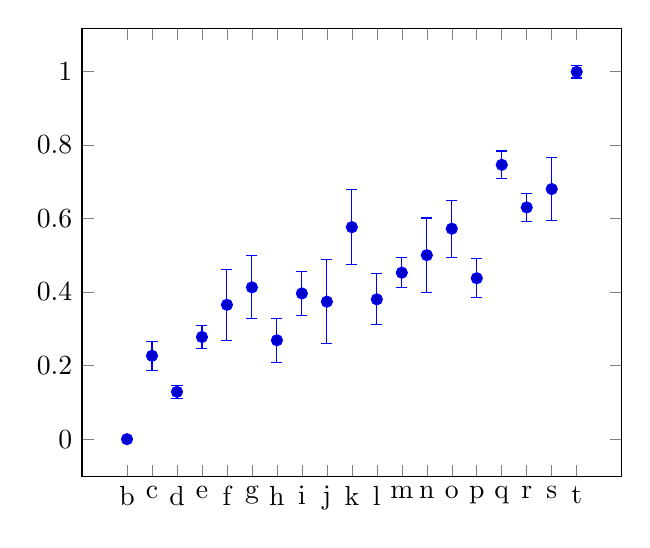
\begin{tikzpicture}
\begin{axis}[%
	%grid=both,%
	%xmajorgrids,%
	xtick={1,2,3,4,5,6,7,8,9,10,11,12,13,14,15,16,17,18,19},%
	xticklabels={b,c,d,e,f,g,h,i,j,k,l,m,n,o,p,q,r,s,t},%
]
% Line plot
\addplot
	plot[ 	%smooth,
	   		only marks,
	      	error bars/.cd,
	      	y dir=both, y explicit %
		]
	coordinates{
	(1,0) 			+- (0,0)
	(2,0.226697)	+- (0,0.0389)
	(3,0.128649)	+- (0,0.0174)
	(4,0.277819)	+- (0,0.0316)
	(5,0.365309) 	+- (0,0.0960)
	(6,0.412726)	+- (0,0.0856)
	(7,0.268849) 	+- (0,0.0598)
	(8,0.396237)	+- (0,0.0589)
	(9,0.373823)	+- (0,0.1148)
	(10,0.576375)	+- (0,0.1020)
	(11,0.380172) 	+- (0,0.0696)
	(12,0.452672)	+- (0,0.0404)
	(13,0.500303)	+- (0,0.1010)
	(14,0.572158)	+- (0,0.0778)
	(15,0.437586)	+- (0,0.0524)
	(16,0.745885)	+- (0,0.0376)
	(17,0.630023)	+- (0,0.0386)
	(18,0.679989)	+- (0,0.0852)
	(19,0.998734)	+- (0,0.0169)
};

\end{axis}
\end{tikzpicture}


% plot erstellt mit MATLAB-File p:\doc\MATLAB\WFS-CompareDMPs\wfs_Compare2008c.m (FromToTo = 1:5:1024)
% und matlab2tikz

%[ 1:19;std(NormCumulativeError);mean(NormCumulativeError)]
%
%ans =
%
%  Columns 1 through 12
%
%    1.0000    2.0000    3.0000    4.0000    5.0000    6.0000    7.0000    8.0000    9.0000   10.0000   11.0000   12.0000
%         0    0.0389    0.0174    0.0316    0.0960    0.0856    0.0598    0.0589    0.1148    0.1020    0.0696    0.0404
%         0    0.2267    0.1286    0.2778    0.3653    0.4127    0.2688    0.3962    0.3738    0.5764    0.3802    0.4527
%
%  Columns 13 through 19
%
%   13.0000   14.0000   15.0000   16.0000   17.0000   18.0000   19.0000
%    0.1010    0.0778    0.0524    0.0376    0.0386    0.0852    0.0169
%    0.5003    0.5722    0.4376    0.7459    0.6300    0.6800    0.9987          	
         	
%
%\end{preview}
%\end{document}%
		\label{fig:NormalizedErrorPlot}%
	\end{figure}%
\else
	\begin{figure}[htp]
		\centering
		%\documentclass{article}
%\usepackage{tikz,pgfplots}
%\usepackage[pdftex,active,tightpage]{preview}
%\begin{document}
%\begin{preview}

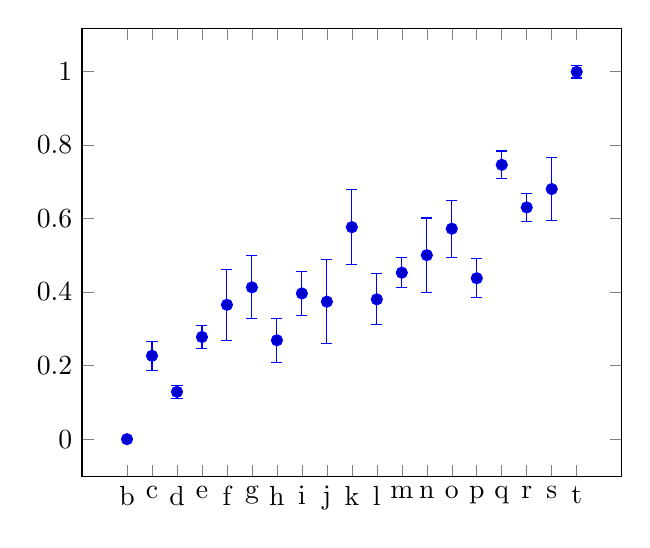
\begin{tikzpicture}
\begin{axis}[%
	%grid=both,%
	%xmajorgrids,%
	xtick={1,2,3,4,5,6,7,8,9,10,11,12,13,14,15,16,17,18,19},%
	xticklabels={b,c,d,e,f,g,h,i,j,k,l,m,n,o,p,q,r,s,t},%
]
% Line plot
\addplot
	plot[ 	%smooth,
	   		only marks,
	      	error bars/.cd,
	      	y dir=both, y explicit %
		]
	coordinates{
	(1,0) 			+- (0,0)
	(2,0.226697)	+- (0,0.0389)
	(3,0.128649)	+- (0,0.0174)
	(4,0.277819)	+- (0,0.0316)
	(5,0.365309) 	+- (0,0.0960)
	(6,0.412726)	+- (0,0.0856)
	(7,0.268849) 	+- (0,0.0598)
	(8,0.396237)	+- (0,0.0589)
	(9,0.373823)	+- (0,0.1148)
	(10,0.576375)	+- (0,0.1020)
	(11,0.380172) 	+- (0,0.0696)
	(12,0.452672)	+- (0,0.0404)
	(13,0.500303)	+- (0,0.1010)
	(14,0.572158)	+- (0,0.0778)
	(15,0.437586)	+- (0,0.0524)
	(16,0.745885)	+- (0,0.0376)
	(17,0.630023)	+- (0,0.0386)
	(18,0.679989)	+- (0,0.0852)
	(19,0.998734)	+- (0,0.0169)
};

\end{axis}
\end{tikzpicture}


% plot erstellt mit MATLAB-File p:\doc\MATLAB\WFS-CompareDMPs\wfs_Compare2008c.m (FromToTo = 1:5:1024)
% und matlab2tikz

%[ 1:19;std(NormCumulativeError);mean(NormCumulativeError)]
%
%ans =
%
%  Columns 1 through 12
%
%    1.0000    2.0000    3.0000    4.0000    5.0000    6.0000    7.0000    8.0000    9.0000   10.0000   11.0000   12.0000
%         0    0.0389    0.0174    0.0316    0.0960    0.0856    0.0598    0.0589    0.1148    0.1020    0.0696    0.0404
%         0    0.2267    0.1286    0.2778    0.3653    0.4127    0.2688    0.3962    0.3738    0.5764    0.3802    0.4527
%
%  Columns 13 through 19
%
%   13.0000   14.0000   15.0000   16.0000   17.0000   18.0000   19.0000
%    0.1010    0.0778    0.0524    0.0376    0.0386    0.0852    0.0169
%    0.5003    0.5722    0.4376    0.7459    0.6300    0.6800    0.9987          	
         	
%
%\end{preview}
%\end{document}
		\caption{%
			Plot of normalized difference Value ($E_{i_{norm}}$, blue diamonds) for the 19 scanned protocols overlaid over Quality-plot (red dots) obtained from the simulation. The normalized Error has been calculated using the difference image of each protocol $i$ with protocol B. The error bars for each protocol show the standard deviation of the error calculated for 205 of the 1024 slices. Note that the scale of the error was normalized to 20--\SI{100}{\percent}, so that both the quality from the simulation and the error are directly comparable. The abscissa shows the scanning time in percentage of time used for the gold standard scan. Protocol T corresponds to the fastest scanning time, protocol B to the slowest. The protocols in between are shown in decreasing order from T--B for increasing percentage of the scanning time.%
		}%
		\label{fig:NormalizedErrorPlot}
	\end{figure}
\fi

\subsubsection{three-dimensional visualization of different protocols}
\label{subsec:comparison}
x	The tomograms of the different protocols were three-dimensionally analyzed and visualized using MeVisLab (Version 2.0 (2009-06-09 Release), MeVis Medical Solutions AG and Fraunhofer MEVIS - Institute for Medical Image Computing, Bremen, Germany). Airway segments were extracted using a threshold interval based region growing algorithm. A seed point for the region growing algorithm was manually defined in the most proximal slice for each independent airway segment. The coordinates of the seed points were kept constant for protocol B--T, allowing direct comparison between the airway segment reconstructions of the different protocols. Airway segments extracted for protocol B, L and T are shown in figure~\ref{fig:BvsT}.

The data shown in figure~\ref{fig:BvsT} represent three of the 19 scanned protocols. Protocol B corresponds to a slightly oversampled gold standard scan, obtained with 15732 projections for all three subscans, recorded in \SI{66}{\minute}. Protocol L was obtained in \SI{35}{\minute} with total 7866 projections. Protocol T was obtained in \SI{12}{\minute} with total 2185 projections. The tomographic dataset from protocol B was reconstructed from 5244 merged projection images, the dataset from protocol L was reconstructed from 2622 merged projections and the dataset from protocol T was reconstructed using only 874 merged projections. Even though protocols L and T were scanned while violating the sampling theorem and with a total scanning time reduction of \SI{40}{\percent} (or more than \SI{86}{\percent}), the samples still appear to be identical to the gold standard protocol in the low-resolution three-dimensional visualization, as shown in figure~\ref{fig:BvsT}(a), (b) and (c).

Obviously, the artifacts introduced through the reduction in scanning time only become apparent at higher magnification. The blue cube inside the green airway segments in figures~\ref{fig:BvsT}(a), (b) and (c) are shown as isosurface visualizations of the lung tissue (which corresponds exactly to the negative of the extracted airway segment) in figures~\ref{fig:BvsT}(d), (e) and (f). The regions of interest show a cube with a side length of \SI{379}{\micro\meter} or 256 pixels.

Even with the higher magnification, the reconstruction of protocol L in figure~\ref{fig:BvsT}(e) appears nearly identical to the reconstruction of the region of interest of protocol B (fig.~\ref{fig:BvsT}(d)). The isosurface of the region of interest of protocol T shown in figure~\ref{fig:BvsT}(f) appears rougher than the isosurface of protocol B. This roughness is introduced through wave-like artifacts visible in the original slice of the dataset of protocol T (not shown). These artifacts arise through the breaching of the sampling theorem, since only 874 projections were acquired for the two ring-scans instead of the 5139 projections ($(3072-200)\frac{\pi}{2}$) required to satisfy the sampling theorem. However, even with this strong undersampling, segmentation, three-dimensional reconstruction and visualization of the sample is still possible.

\ifiucr%%% iucr %%%
%\onecolumn
	\begin{figure}
		\caption{%
			Comparison of three-dimensional visualizations of protocols B, L and T. %
			(a) Three independent airway segments (green, red, yellow) of Protocol B were extracted using a region growing algorithm. %
			(b) Same for protocol L. %
			(c) Same for protocol T. A cubical region of interest (ROI, blue) with a side length of 256 pixels (corresponding to \SI{379}{\micro\meter}) is marked inside the leftmost segment for all protocols. %
			(d): Detailed view of isosurfaces of the lung tissue inside the ROIs shown for protocol B. %
			(e): Same for protocol L.
			(f): Same for protocol T. Note the artifacts in the isosurface in subfigure (e) and (f).%
			}%
		\renewcommand{\imsize}{.33\linewidth}%
		\pgfmathsetlength{\imagewidth}{\imsize}%
		\pgfmathsetlength{\imagescale}{\imagewidth/1085}%
		\def\x{551} % scalebar-x at golden ratio of x=1085px (671px = golden ratio: 551 is set to fit the one-column-width in the draft mode!!!)
		\def\y{530} % scalebar-y at 90% of height of y=589px
		\begin{tikzpicture}[x=\imagescale,y=-\imagescale]
			\node[anchor=north west, inner sep=0pt, outer sep=0pt] at (0,0)
				{\includegraphics[width=\imagewidth]{img/comparisonBvsT/ob}};
			% 1030px = 2.627mm > 100px = 255um > 196px = 500um
%			\draw[|-|,thick] (30,339) -- (1054,454) node [white,sloped,midway,above] {\SI{2.627}{\milli\meter} (1775px)};
			\draw [|-|,thick] (\x,\y) -- (\x+196,\y) node [fill=white,semitransparent,right] {\SI{500}{\micro\meter}} node [right] {\SI{500}{\micro\meter}};
			\node [fill=white,semitransparent,anchor=south west] at (0,589) {(a)};
			\node [anchor=south west] at (0,589) {(a)};
		\end{tikzpicture}%
		\begin{tikzpicture}[x=\imagescale,y=-\imagescale]%
			\node[anchor=north west, inner sep=0pt, outer sep=0pt] at (0,0)
				{\includegraphics[width=\imagewidth]{img/comparisonBvsT/ol}};
			% 1030px = 2.627mm > 100px = 255um > 196px = 500um
			\draw [|-|,thick] (\x,\y) -- (\x+196,\y) node [fill=white,semitransparent,right] {\SI{500}{\micro\meter}} node [right] {\SI{500}{\micro\meter}};
			\node [fill=white,semitransparent,anchor=south west] at (0,589) {(b)};
			\node [anchor=south west] at (0,589) {(b)};
		\end{tikzpicture}%
		\begin{tikzpicture}[x=\imagescale,y=-\imagescale]%
			\node[anchor=north west, inner sep=0pt, outer sep=0pt] at (0,0)
				{\includegraphics[width=\imagewidth]{img/comparisonBvsT/ot}};
			% 1030px = 2.627mm > 100px = 255um > 196px = 500um
			\draw [|-|,thick] (\x,\y) -- (\x+196,\y) node [fill=white,semitransparent,right] {\SI{500}{\micro\meter}} node [right] {\SI{500}{\micro\meter}};
			\node [fill=white,semitransparent,anchor=south west] at (0,589) {(c)};
			\node [anchor=south west] at (0,589) {(c)};
		\end{tikzpicture}%
		\\%
		\pgfmathsetlength{\imagewidth}{\imsize}%
		\pgfmathsetlength{\imagescale}{\imagewidth/816}%
		\def\x{504} % scalebar-x at golden ratio of x=816px
		\def\y{734} % scalebar-y at 90% of height of y=815px
		\begin{tikzpicture}[x=\imagescale,y=-\imagescale]%
			\node[anchor=north west, inner sep=0pt, outer sep=0pt] at (0,0)
				{\includegraphics[width=\imagewidth]{img/comparisonBvsT/roiB}};
			% 761px = 0.37888mm > 100px = 50um > 100.4px = 500um
%			\draw[|-|,thick] (792,438) -- (31,435) node [sloped,midway,above] {\SI{378.88}{\micro\meter} (256px)};
			\draw[|-|,thick] (\x,\y) -- (\x+100.4,\y) node [fill=white,semitransparent,right] {\SI{50}{\micro\meter}} node [right] {\SI{50}{\micro\meter}};
			\node [fill=white,semitransparent,anchor=south west] at (0,815) {(d)};
			\node [anchor=south west] at (0,815) {(d)};
	\end{tikzpicture}%
		\begin{tikzpicture}[x=\imagescale,y=-\imagescale]%
			\node[anchor=north west, inner sep=0pt, outer sep=0pt] at (0,0)
				{\includegraphics[width=\imagewidth]{img/comparisonBvsT/roiL}};
			% 761px = 0.37888mm > 100px = 50um > 100.4px = 500um
			\draw[|-|,thick] (\x,\y) -- (\x+100.4,\y) node [fill=white,semitransparent,right] {\SI{50}{\micro\meter}} node [right] {\SI{50}{\micro\meter}};
			\node [fill=white,semitransparent,anchor=south west] at (0,815) {(e)};
			\node [anchor=south west] at (0,815) {(e)};
		\end{tikzpicture}%
		\begin{tikzpicture}[x=\imagescale,y=-\imagescale]%
			\node[anchor=north west, inner sep=0pt, outer sep=0pt] at (0,0)
				{\includegraphics[width=\imagewidth]{img/comparisonBvsT/roiT}};
			% 761px = 0.37888mm > 100px = 50um > 100.4px = 500um
			\draw[|-|,thick] (\x,\y) -- (\x+100.4,\y) node [fill=white,semitransparent,right] {\SI{50}{\micro\meter}} node [right] {\SI{50}{\micro\meter}};
			\node [fill=white,semitransparent,anchor=south west] at (0,815) {(f)};
			\node [anchor=south west] at (0,815) {(f)};
		\end{tikzpicture}%
		\label{fig:BvsT}%
	\end{figure}%
%\twocolumn%
\else%
	\begin{figure}[htp]
		\centering
		\renewcommand{\imsize}{.333\linewidth}%
		\includegraphics[width=\imagewidth]{img/comparisonBvsT/ob}%
		\includegraphics[width=\imagewidth]{img/comparisonBvsT/ol}%
		\includegraphics[width=\imagewidth]{img/comparisonBvsT/ot}%
		\\%
		\includegraphics[width=\imagewidth]{img/comparisonBvsT/roiB}%
		\includegraphics[width=\imagewidth]{img/comparisonBvsT/roiL}%
		\includegraphics[width=\imagewidth]{img/comparisonBvsT/roiT}%
		\caption{%
			Comparison of three-dimensional visualizations of protocols B, L and T. %
			(a) Three independent airway segments (green, red, yellow) of Protocol B were extracted using a region growing algorithm. %
			(b) Same for protocol L. %
			(c) Same for protocol T. A cubical region of interest (ROI, blue) with a side length of 256 pixels (corresponding to \SI{379}{\micro\meter}) is marked inside the leftmost segment for all protocols. %
			(d): Detailed view of isosurfaces of the lung tissue inside the ROIs shown for protocol B. %
			(e): Same for protocol L.
			(f): Same for protocol T. Note the artifacts in the isosurface in subfigure (e) and (f).%
			}%
		\label{fig:BvsT}%
	\end{figure}
\fi%

For further analysis four regions of interest with a side length of 256 pixels (at \SI{1.48}{\micro\meter\per pixel}, thus containing a volume of \SI{1.678e7}{voxels}) have been extracted for each of the protocols B, L and T. The three-dimensional placement of these ROIs inside the sample is shown in figure~\ref{fig:roi3d}. Each of the ROIs has been binarized using an automatically determined threshold~\cite{Otsu1979} and small particles inside the segmented airspace lumen have been removed using a connected components analysis. Subsequently, the euclidean distance transformation has been calculated for each thresholded ROI.

\renewcommand{\imsize}{\columnwidth}
\begin{figure}%
	\centering%
	\pgfmathsetlength{\imagewidth}{\imsize}%
	\pgfmathsetlength{\imagescale}{\imagewidth/1452}%
	\caption{Overview of the placement of the four regions of interest where the histogram of the euclidean distance transformation distribution has been calculated. Grey: Semitransparent volume rendering of the lung tissue sample. Red: Four regions of interest, extracted to calculate the distance transformation, each with a side-length of 256 pixels. The labels of the ROIs conform to the legends in figure~\ref{fig:DTFplots}.}%
	\begin{tikzpicture}[x=\imagescale,y=-\imagescale]
		\def\x{297} % scalebar-x at golden ratio of x=1452px
		\def\y{684} % scalebar-y at 90% of height of y=760px
		\node[anchor=north west, inner sep=0pt, outer sep=0pt] at (0,0)
	     {\includegraphics[width=\imagewidth]{img/dtf-roi/ROIs-3d}};
		% 1357px = 4.0138mm > 100px = 296um > 169px = 500um
		% \draw[|-|,thick,red] (83,517) -- (1425,719) node [sloped,midway,below] {\SI{4.0138}{\milli\meter} (2712px)};
		\draw[|-|,thick] (\x,\y) -- (\x+169,\y) node [midway, above] {\SI{500}{\micro\meter}};
		\draw[|-|,thick, white] (\x+645,\y-180) -- (\x+645+128,\y-180) node [midway, below] {\SI{256}{pixels}};
		\draw ( 368,360) node [fill=white, semitransparent] {ROI 1} node {ROI 1};
		\draw (1038,312) node [fill=white, semitransparent] {ROI 2} node {ROI 2};
		\draw ( 767,413) node [fill=white, semitransparent] {ROI 3} node {ROI 3};
		\draw ( 684,139) node [fill=white, semitransparent] {ROI 4} node {ROI 4};
	\end{tikzpicture}%
	\label{fig:roi3d}%
\end{figure}

For comparison, the histogram of the euclidean distance transformation has been plotted for all four regions of interest in each protocol (B, L and T).

\renewcommand{\imsize}{.309\columnwidth}
%\onecolumn
\begin{figure}%
	\centering
	\caption{Histogram-Plots for each of the of 4 ROIs, each showing the histogram of the distance transformation for the protocols B, L and T.}%		
	\begin{tabular}{cc}%
		% \documentclass{article}
% \usepackage{tikz,pgfplots}
% \usepackage[pdftex,active,tightpage]{preview}
% \begin{document}
% \begin{preview}
%%%%%%%%%%%%
\begin{tikzpicture}
\begin{semilogyaxis}[
% axis on top,
% scale only axis,
grid=both,
width=\imsize,
% height=3.56562in,
xmin=0, xmax=65,
ymin=1, ymax=1e+007,
xlabel={Thickness [\micro m]},
ylabel={Number of Voxels},
% title={ROI 1},
legend entries={B (ROI 1),L (ROI 1),T (ROI 1)}
]

\addplot [
color=blue,
solid
]coordinates{
 (1.036,0) (1.036,1.25111e+006) (1.036,1.25111e+006) (1.184,1.25111e+006) (1.184,0)%
 (1.332,0) (1.332,615061) (1.332,615061) (1.48,615061) (1.48,0)%
 (1.776,0) (1.776,260078) (1.776,260078) (1.924,260078) (1.924,0)%
 (2.072,0) (2.072,311501) (2.072,311501) (2.22,311501) (2.22,487193) (2.22,487193) (2.368,487193) (2.368,0)%
 (2.516,0) (2.516,247233) (2.516,247233) (2.664,247233) (2.664,0)%
 (2.812,0) (2.812,262874) (2.812,262874) (2.96,262874) (2.96,0)%
 (3.108,0) (3.108,362647) (3.108,362647) (3.256,362647) (3.256,177701) (3.256,177701) (3.404,177701) (3.404,143434) (3.404,143434) (3.552,143434) (3.552,73909) (3.552,73909) (3.7,73909) (3.7,216769) (3.7,216769) (3.848,216769) (3.848,205224) (3.848,205224) (3.996,205224) (3.996,0)%
 (4.144,0) (4.144,379292) (4.144,379292) (4.292,379292) (4.292,144948) (4.292,144948) (4.44,144948) (4.44,79396) (4.44,79396) (4.588,79396) (4.588,102403) (4.588,102403) (4.736,102403) (4.736,209710) (4.736,209710) (4.884,209710) (4.884,0)%
 (5.032,0) (5.032,289501) (5.032,289501) (5.18,289501) (5.18,168870) (5.18,168870) (5.328,168870) (5.328,65511) (5.328,65511) (5.476,65511) (5.476,185453) (5.476,185453) (5.624,185453) (5.624,74694) (5.624,74694) (5.772,74694) (5.772,52846) (5.772,52846) (5.92,52846) (5.92,230325) (5.92,230325) (6.068,230325) (6.068,70838) (6.068,70838) (6.216,70838) (6.216,127584) (6.216,127584) (6.364,127584) (6.364,112007) (6.364,112007) (6.512,112007) (6.512,220564) (6.512,220564) (6.66,220564) (6.66,83095) (6.66,83095) (6.808,83095) (6.808,140906) (6.808,140906) (6.956,140906) (6.956,46921) (6.956,46921) (7.104,46921) (7.104,98956) (7.104,98956) (7.252,98956) (7.252,191119) (7.252,191119) (7.4,191119) (7.4,109497) (7.4,109497) (7.548,109497) (7.548,83683) (7.548,83683) (7.696,83683) (7.696,95212) (7.696,95212) (7.844,95212) (7.844,98242) (7.844,98242) (7.992,98242) (7.992,85358) (7.992,85358) (8.14,85358) (8.14,69667) (8.14,69667) (8.288,69667) (8.288,193089) (8.288,193089) (8.436,193089) (8.436,60959) (8.436,60959) (8.584,60959) (8.584,87206) (8.584,87206) (8.732,87206) (8.732,88163) (8.732,88163) (8.88,88163) (8.88,111357) (8.88,111357) (9.028,111357) (9.028,94851) (9.028,94851) (9.176,94851) (9.176,28137) (9.176,28137) (9.324,28137) (9.324,151541) (9.324,151541) (9.472,151541) (9.472,121345) (9.472,121345) (9.62,121345) (9.62,14476) (9.62,14476) (9.768,14476) (9.768,148633) (9.768,148633) (9.916,148633) (9.916,68210) (9.916,68210) (10.064,68210) (10.064,51398) (10.064,51398) (10.212,51398) (10.212,114875) (10.212,114875) (10.36,114875) (10.36,79729) (10.36,79729) (10.508,79729) (10.508,68479) (10.508,68479) (10.656,68479) (10.656,72250) (10.656,72250) (10.804,72250) (10.804,72049) (10.804,72049) (10.952,72049) (10.952,79753) (10.952,79753) (11.1,79753) (11.1,81664) (11.1,81664) (11.248,81664) (11.248,34829) (11.248,34829) (11.396,34829) (11.396,90607) (11.396,90607) (11.544,90607) (11.544,86063) (11.544,86063) (11.692,86063) (11.692,69170) (11.692,69170) (11.84,69170) (11.84,53271) (11.84,53271) (11.988,53271) (11.988,83343) (11.988,83343) (12.136,83343) (12.136,49082) (12.136,49082) (12.284,49082) (12.284,32539) (12.284,32539) (12.432,32539) (12.432,111026) (12.432,111026) (12.58,111026) (12.58,63768) (12.58,63768) (12.728,63768) (12.728,62827) (12.728,62827) (12.876,62827) (12.876,51868) (12.876,51868) (13.024,51868) (13.024,48185) (13.024,48185) (13.172,48185) (13.172,62312) (13.172,62312) (13.32,62312) (13.32,45697) (13.32,45697) (13.468,45697) (13.468,59199) (13.468,59199) (13.616,59199) (13.616,50125) (13.616,50125) (13.764,50125) (13.764,61532) (13.764,61532) (13.912,61532) (13.912,48789) (13.912,48789) (14.06,48789) (14.06,54360) (14.06,54360) (14.208,54360) (14.208,32444) (14.208,32444) (14.356,32444) (14.356,65857) (14.356,65857) (14.504,65857) (14.504,51861) (14.504,51861) (14.652,51861) (14.652,45863) (14.652,45863) (14.8,45863) (14.8,47039) (14.8,47039) (14.948,47039) (14.948,53244) (14.948,53244) (15.096,53244) (15.096,30468) (15.096,30468) (15.244,30468) (15.244,36249) (15.244,36249) (15.392,36249) (15.392,43946) (15.392,43946) (15.54,43946) (15.54,63584) (15.54,63584) (15.688,63584) (15.688,40905) (15.688,40905) (15.836,40905) (15.836,49551) (15.836,49551) (15.984,49551) (15.984,31017) (15.984,31017) (16.132,31017) (16.132,44626) (16.132,44626) (16.28,44626) (16.28,45134) (16.28,45134) (16.428,45134) (16.428,19390) (16.428,19390) (16.576,19390) (16.576,48419) (16.576,48419) (16.724,48419) (16.724,40598) (16.724,40598) (16.872,40598) (16.872,43419) (16.872,43419) (17.02,43419) (17.02,33352) (17.02,33352) (17.168,33352) (17.168,31319) (17.168,31319) (17.316,31319) (17.316,32941) (17.316,32941) (17.464,32941) (17.464,27127) (17.464,27127) (17.612,27127) (17.612,52285) (17.612,52285) (17.76,52285) (17.76,34413) (17.76,34413) (17.908,34413) (17.908,27138) (17.908,27138) (18.056,27138) (18.056,38339) (18.056,38339) (18.204,38339) (18.204,24127) (18.204,24127) (18.352,24127) (18.352,38567) (18.352,38567) (18.5,38567) (18.5,27187) (18.5,27187) (18.648,27187) (18.648,48367) (18.648,48367) (18.796,48367) (18.796,24372) (18.796,24372) (18.944,24372) (18.944,28211) (18.944,28211) (19.092,28211) (19.092,32657) (19.092,32657) (19.24,32657) (19.24,33653) (19.24,33653) (19.388,33653) (19.388,23533) (19.388,23533) (19.536,23533) (19.536,19206) (19.536,19206) (19.684,19206) (19.684,42551) (19.684,42551) (19.832,42551) (19.832,27399) (19.832,27399) (19.98,27399) (19.98,31332) (19.98,31332) (20.128,31332) (20.128,21042) (20.128,21042) (20.276,21042) (20.276,23662) (20.276,23662) (20.424,23662) (20.424,30551) (20.424,30551) (20.572,30551) (20.572,23126) (20.572,23126) (20.72,23126) (20.72,32415) (20.72,32415) (20.868,32415) (20.868,26522) (20.868,26522) (21.016,26522) (21.016,22807) (21.016,22807) (21.164,22807) (21.164,20796) (21.164,20796) (21.312,20796) (21.312,31838) (21.312,31838) (21.46,31838) (21.46,21486) (21.46,21486) (21.608,21486) (21.608,17839) (21.608,17839) (21.756,17839) (21.756,29346) (21.756,29346) (21.904,29346) (21.904,25394) (21.904,25394) (22.052,25394) (22.052,23931) (22.052,23931) (22.2,23931) (22.2,19010) (22.2,19010) (22.348,19010) (22.348,20692) (22.348,20692) (22.496,20692) (22.496,19154) (22.496,19154) (22.644,19154) (22.644,18638) (22.644,18638) (22.792,18638) (22.792,29391) (22.792,29391) (22.94,29391) (22.94,15838) (22.94,15838) (23.088,15838) (23.088,21447) (23.088,21447) (23.236,21447) (23.236,22688) (23.236,22688) (23.384,22688) (23.384,15210) (23.384,15210) (23.532,15210) (23.532,21187) (23.532,21187) (23.68,21187) (23.68,13291) (23.68,13291) (23.828,13291) (23.828,22614) (23.828,22614) (23.976,22614) (23.976,19969) (23.976,19969) (24.124,19969) (24.124,16789) (24.124,16789) (24.272,16789) (24.272,17367) (24.272,17367) (24.42,17367) (24.42,15681) (24.42,15681) (24.568,15681) (24.568,19884) (24.568,19884) (24.716,19884) (24.716,9854) (24.716,9854) (24.864,9854) (24.864,20652) (24.864,20652) (25.012,20652) (25.012,16546) (25.012,16546) (25.16,16546) (25.16,16711) (25.16,16711) (25.308,16711) (25.308,13728) (25.308,13728) (25.456,13728) (25.456,12229) (25.456,12229) (25.604,12229) (25.604,15340) (25.604,15340) (25.752,15340) (25.752,10601) (25.752,10601) (25.9,10601) (25.9,20681) (25.9,20681) (26.048,20681) (26.048,12315) (26.048,12315) (26.196,12315) (26.196,14426) (26.196,14426) (26.344,14426) (26.344,12931) (26.344,12931) (26.492,12931) (26.492,14507) (26.492,14507) (26.64,14507) (26.64,11234) (26.64,11234) (26.788,11234) (26.788,11937) (26.788,11937) (26.936,11937) (26.936,13626) (26.936,13626) (27.084,13626) (27.084,13537) (27.084,13537) (27.232,13537) (27.232,11925) (27.232,11925) (27.38,11925) (27.38,12930) (27.38,12930) (27.528,12930) (27.528,9601) (27.528,9601) (27.676,9601) (27.676,9149) (27.676,9149) (27.824,9149) (27.824,10962) (27.824,10962) (27.972,10962) (27.972,12041) (27.972,12041) (28.12,12041) (28.12,10697) (28.12,10697) (28.268,10697) (28.268,11133) (28.268,11133) (28.416,11133) (28.416,9424) (28.416,9424) (28.564,9424) (28.564,9013) (28.564,9013) (28.712,9013) (28.712,12315) (28.712,12315) (28.86,12315) (28.86,7887) (28.86,7887) (29.008,7887) (29.008,9301) (29.008,9301) (29.156,9301) (29.156,9182) (29.156,9182) (29.304,9182) (29.304,9502) (29.304,9502) (29.452,9502) (29.452,7621) (29.452,7621) (29.6,7621) (29.6,9584) (29.6,9584) (29.748,9584) (29.748,6208) (29.748,6208) (29.896,6208) (29.896,7255) (29.896,7255) (30.044,7255) (30.044,11315) (30.044,11315) (30.192,11315) (30.192,8066) (30.192,8066) (30.34,8066) (30.34,7519) (30.34,7519) (30.488,7519) (30.488,6584) (30.488,6584) (30.636,6584) (30.636,6964) (30.636,6964) (30.784,6964) (30.784,6797) (30.784,6797) (30.932,6797) (30.932,5566) (30.932,5566) (31.08,5566) (31.08,7473) (31.08,7473) (31.228,7473) (31.228,7186) (31.228,7186) (31.376,7186) (31.376,5091) (31.376,5091) (31.524,5091) (31.524,7039) (31.524,7039) (31.672,7039) (31.672,5524) (31.672,5524) (31.82,5524) (31.82,5297) (31.82,5297) (31.968,5297) (31.968,4091) (31.968,4091) (32.116,4091) (32.116,7392) (32.116,7392) (32.264,7392) (32.264,5227) (32.264,5227) (32.412,5227) (32.412,5764) (32.412,5764) (32.56,5764) (32.56,4223) (32.56,4223) (32.708,4223) (32.708,4689) (32.708,4689) (32.856,4689) (32.856,4919) (32.856,4919) (33.004,4919) (33.004,4045) (33.004,4045) (33.152,4045) (33.152,5036) (33.152,5036) (33.3,5036) (33.3,4647) (33.3,4647) (33.448,4647) (33.448,4661) (33.448,4661) (33.596,4661) (33.596,3201) (33.596,3201) (33.744,3201) (33.744,5155) (33.744,5155) (33.892,5155) (33.892,3256) (33.892,3256) (34.04,3256) (34.04,3062) (34.04,3062) (34.188,3062) (34.188,5112) (34.188,5112) (34.336,5112) (34.336,3688) (34.336,3688) (34.484,3688) (34.484,3215) (34.484,3215) (34.632,3215) (34.632,3841) (34.632,3841) (34.78,3841) (34.78,3096) (34.78,3096) (34.928,3096) (34.928,3620) (34.928,3620) (35.076,3620) (35.076,2830) (35.076,2830) (35.224,2830) (35.224,3711) (35.224,3711) (35.372,3711) (35.372,3323) (35.372,3323) (35.52,3323) (35.52,2678) (35.52,2678) (35.668,2678) (35.668,3506) (35.668,3506) (35.816,3506) (35.816,2545) (35.816,2545) (35.964,2545) (35.964,2722) (35.964,2722) (36.112,2722) (36.112,2407) (36.112,2407) (36.26,2407) (36.26,3437) (36.26,3437) (36.408,3437) (36.408,2471) (36.408,2471) (36.556,2471) (36.556,2523) (36.556,2523) (36.704,2523) (36.704,2558) (36.704,2558) (36.852,2558) (36.852,2415) (36.852,2415) (37,2415) (37,1949) (37,1949) (37.148,1949) (37.148,2253) (37.148,2253) (37.296,2253) (37.296,2855) (37.296,2855) (37.444,2855) (37.444,2187) (37.444,2187) (37.592,2187) (37.592,2267) (37.592,2267) (37.74,2267) (37.74,1759) (37.74,1759) (37.888,1759) (37.888,1684) (37.888,1684) (38.036,1684) (38.036,2203) (38.036,2203) (38.184,2203) (38.184,1671) (38.184,1671) (38.332,1671) (38.332,2267) (38.332,2267) (38.48,2267) (38.48,2018) (38.48,2018) (38.628,2018) (38.628,1378) (38.628,1378) (38.776,1378) (38.776,1776) (38.776,1776) (38.924,1776) (38.924,1973) (38.924,1973) (39.072,1973) (39.072,1539) (39.072,1539) (39.22,1539) (39.22,1075) (39.22,1075) (39.368,1075) (39.368,2143) (39.368,2143) (39.516,2143) (39.516,1159) (39.516,1159) (39.664,1159) (39.664,1639) (39.664,1639) (39.812,1639) (39.812,1331) (39.812,1331) (39.96,1331) (39.96,1411) (39.96,1411) (40.108,1411) (40.108,1181) (40.108,1181) (40.256,1181) (40.256,1310) (40.256,1310) (40.404,1310) (40.404,1538) (40.404,1538) (40.552,1538) (40.552,1074) (40.552,1074) (40.7,1074) (40.7,1274) (40.7,1274) (40.848,1274) (40.848,989) (40.848,989) (40.996,989) (40.996,1195) (40.996,1195) (41.144,1195) (41.144,906) (41.144,906) (41.292,906) (41.292,1026) (41.292,1026) (41.44,1026) (41.44,1201) (41.44,1201) (41.588,1201) (41.588,959) (41.588,959) (41.736,959) (41.736,987) (41.736,987) (41.884,987) (41.884,924) (41.884,924) (42.032,924) (42.032,667) (42.032,667) (42.18,667) (42.18,941) (42.18,941) (42.328,941) (42.328,544) (42.328,544) (42.476,544) (42.476,1026) (42.476,1026) (42.624,1026) (42.624,842) (42.624,842) (42.772,842) (42.772,726) (42.772,726) (42.92,726) (42.92,573) (42.92,573) (43.068,573) (43.068,717) (43.068,717) (43.216,717) (43.216,638) (43.216,638) (43.364,638) (43.364,597) (43.364,597) (43.512,597) (43.512,693) (43.512,693) (43.66,693) (43.66,657) (43.66,657) (43.808,657) (43.808,480) (43.808,480) (43.956,480) (43.956,673) (43.956,673) (44.104,673) (44.104,466) (44.104,466) (44.252,466) (44.252,580) (44.252,580) (44.4,580) (44.4,414) (44.4,414) (44.548,414) (44.548,657) (44.548,657) (44.696,657) (44.696,454) (44.696,454) (44.844,454) (44.844,591) (44.844,591) (44.992,591) (44.992,422) (44.992,422) (45.14,422) (45.14,428) (45.14,428) (45.288,428) (45.288,353) (45.288,353) (45.436,353) (45.436,452) (45.436,452) (45.584,452) (45.584,483) (45.584,483) (45.732,483) (45.732,413) (45.732,413) (45.88,413) (45.88,411) (45.88,411) (46.028,411) (46.028,320) (46.028,320) (46.176,320) (46.176,397) (46.176,397) (46.324,397) (46.324,359) (46.324,359) (46.472,359) (46.472,305) (46.472,305) (46.62,305) (46.62,328) (46.62,328) (46.768,328) (46.768,358) (46.768,358) (46.916,358) (46.916,319) (46.916,319) (47.064,319) (47.064,291) (47.064,291) (47.212,291) (47.212,284) (47.212,284) (47.36,284) (47.36,234) (47.36,234) (47.508,234) (47.508,220) (47.508,220) (47.656,220) (47.656,344) (47.656,344) (47.804,344) (47.804,265) (47.804,265) (47.952,265) (47.952,191) (47.952,191) (48.1,191) (48.1,161) (48.1,161) (48.248,161) (48.248,231) (48.248,231) (48.396,231) (48.396,155) (48.396,155) (48.544,155) (48.544,171) (48.544,171) (48.692,171) (48.692,234) (48.692,234) (48.84,234) (48.84,129) (48.84,129) (48.988,129) (48.988,116) (48.988,116) (49.136,116) (49.136,157) (49.136,157) (49.284,157) (49.284,116) (49.284,116) (49.432,116) (49.432,88) (49.432,88) (49.58,88) (49.58,85) (49.58,85) (49.728,85) (49.728,96) (49.728,96) (49.876,96) (49.876,80) (49.876,80) (50.024,80) (50.024,82) (50.024,82) (50.172,82) (50.172,57) (50.172,57) (50.32,57) (50.32,35) (50.32,35) (50.468,35) (50.468,46) (50.468,46) (50.616,46) (50.616,36) (50.616,36) (50.764,36) (50.764,29) (50.764,29) (50.912,29) (50.912,21) (50.912,21) (51.06,21) (51.06,16) (51.06,16) (51.208,16) (51.208,16) (51.208,16) (51.356,16) (51.356,14) (51.356,14) (51.504,14) (51.504,9) (51.504,9) (51.652,9) (51.652,9) (51.652,9) (51.8,9) (51.8,10) (51.8,10) (51.948,10) (51.948,4) (51.948,4) (52.096,4) (52.096,4) (52.096,4) (52.244,4) (52.244,2) (52.244,2) (52.392,2) (52.392,1)%
 (52.54,1) (52.54,2) (52.54,2) (52.688,2) (52.688,1)
};

\addplot [
color=green,
solid
]coordinates{
 (1.036,0) (1.036,1.25308e+006) (1.036,1.25308e+006) (1.184,1.25308e+006) (1.184,0)%
 (1.332,0) (1.332,613821) (1.332,613821) (1.48,613821) (1.48,0)%
 (1.776,0) (1.776,259899) (1.776,259899) (1.924,259899) (1.924,0)%
 (2.072,0) (2.072,310370) (2.072,310370) (2.22,310370) (2.22,486829) (2.22,486829) (2.368,486829) (2.368,0)%
 (2.516,0) (2.516,247747) (2.516,247747) (2.664,247747) (2.664,0)%
 (2.812,0) (2.812,258533) (2.812,258533) (2.96,258533) (2.96,0)%
 (3.108,0) (3.108,361745) (3.108,361745) (3.256,361745) (3.256,179371) (3.256,179371) (3.404,179371) (3.404,143506) (3.404,143506) (3.552,143506) (3.552,72869) (3.552,72869) (3.7,72869) (3.7,214163) (3.7,214163) (3.848,214163) (3.848,206273) (3.848,206273) (3.996,206273) (3.996,0)%
 (4.144,0) (4.144,376367) (4.144,376367) (4.292,376367) (4.292,144871) (4.292,144871) (4.44,144871) (4.44,79489) (4.44,79489) (4.588,79489) (4.588,101729) (4.588,101729) (4.736,101729) (4.736,209144) (4.736,209144) (4.884,209144) (4.884,0)%
 (5.032,0) (5.032,285587) (5.032,285587) (5.18,285587) (5.18,169714) (5.18,169714) (5.328,169714) (5.328,65682) (5.328,65682) (5.476,65682) (5.476,183620) (5.476,183620) (5.624,183620) (5.624,75379) (5.624,75379) (5.772,75379) (5.772,51642) (5.772,51642) (5.92,51642) (5.92,227882) (5.92,227882) (6.068,227882) (6.068,71053) (6.068,71053) (6.216,71053) (6.216,127295) (6.216,127295) (6.364,127295) (6.364,111638) (6.364,111638) (6.512,111638) (6.512,218480) (6.512,218480) (6.66,218480) (6.66,82720) (6.66,82720) (6.808,82720) (6.808,139178) (6.808,139178) (6.956,139178) (6.956,47263) (6.956,47263) (7.104,47263) (7.104,97436) (7.104,97436) (7.252,97436) (7.252,190870) (7.252,190870) (7.4,190870) (7.4,108250) (7.4,108250) (7.548,108250) (7.548,83492) (7.548,83492) (7.696,83492) (7.696,94695) (7.696,94695) (7.844,94695) (7.844,96844) (7.844,96844) (7.992,96844) (7.992,84074) (7.992,84074) (8.14,84074) (8.14,69652) (8.14,69652) (8.288,69652) (8.288,191832) (8.288,191832) (8.436,191832) (8.436,60244) (8.436,60244) (8.584,60244) (8.584,86981) (8.584,86981) (8.732,86981) (8.732,86728) (8.732,86728) (8.88,86728) (8.88,110216) (8.88,110216) (9.028,110216) (9.028,94312) (9.028,94312) (9.176,94312) (9.176,27164) (9.176,27164) (9.324,27164) (9.324,150953) (9.324,150953) (9.472,150953) (9.472,120343) (9.472,120343) (9.62,120343) (9.62,14202) (9.62,14202) (9.768,14202) (9.768,147009) (9.768,147009) (9.916,147009) (9.916,67351) (9.916,67351) (10.064,67351) (10.064,49810) (10.064,49810) (10.212,49810) (10.212,114108) (10.212,114108) (10.36,114108) (10.36,79775) (10.36,79775) (10.508,79775) (10.508,67677) (10.508,67677) (10.656,67677) (10.656,71054) (10.656,71054) (10.804,71054) (10.804,71112) (10.804,71112) (10.952,71112) (10.952,78892) (10.952,78892) (11.1,78892) (11.1,80222) (11.1,80222) (11.248,80222) (11.248,34643) (11.248,34643) (11.396,34643) (11.396,90088) (11.396,90088) (11.544,90088) (11.544,84851) (11.544,84851) (11.692,84851) (11.692,68051) (11.692,68051) (11.84,68051) (11.84,52909) (11.84,52909) (11.988,52909) (11.988,81863) (11.988,81863) (12.136,81863) (12.136,48703) (12.136,48703) (12.284,48703) (12.284,32105) (12.284,32105) (12.432,32105) (12.432,109750) (12.432,109750) (12.58,109750) (12.58,63514) (12.58,63514) (12.728,63514) (12.728,62172) (12.728,62172) (12.876,62172) (12.876,50881) (12.876,50881) (13.024,50881) (13.024,47091) (13.024,47091) (13.172,47091) (13.172,62039) (13.172,62039) (13.32,62039) (13.32,44968) (13.32,44968) (13.468,44968) (13.468,58587) (13.468,58587) (13.616,58587) (13.616,49966) (13.616,49966) (13.764,49966) (13.764,60443) (13.764,60443) (13.912,60443) (13.912,48528) (13.912,48528) (14.06,48528) (14.06,53901) (14.06,53901) (14.208,53901) (14.208,32302) (14.208,32302) (14.356,32302) (14.356,64503) (14.356,64503) (14.504,64503) (14.504,51449) (14.504,51449) (14.652,51449) (14.652,45907) (14.652,45907) (14.8,45907) (14.8,46182) (14.8,46182) (14.948,46182) (14.948,52795) (14.948,52795) (15.096,52795) (15.096,30334) (15.096,30334) (15.244,30334) (15.244,35498) (15.244,35498) (15.392,35498) (15.392,43463) (15.392,43463) (15.54,43463) (15.54,63129) (15.54,63129) (15.688,63129) (15.688,40290) (15.688,40290) (15.836,40290) (15.836,49459) (15.836,49459) (15.984,49459) (15.984,30485) (15.984,30485) (16.132,30485) (16.132,44159) (16.132,44159) (16.28,44159) (16.28,44784) (16.28,44784) (16.428,44784) (16.428,19043) (16.428,19043) (16.576,19043) (16.576,48026) (16.576,48026) (16.724,48026) (16.724,40100) (16.724,40100) (16.872,40100) (16.872,43361) (16.872,43361) (17.02,43361) (17.02,33092) (17.02,33092) (17.168,33092) (17.168,30961) (17.168,30961) (17.316,30961) (17.316,32607) (17.316,32607) (17.464,32607) (17.464,26918) (17.464,26918) (17.612,26918) (17.612,51725) (17.612,51725) (17.76,51725) (17.76,34420) (17.76,34420) (17.908,34420) (17.908,27015) (17.908,27015) (18.056,27015) (18.056,37899) (18.056,37899) (18.204,37899) (18.204,23839) (18.204,23839) (18.352,23839) (18.352,38670) (18.352,38670) (18.5,38670) (18.5,26977) (18.5,26977) (18.648,26977) (18.648,47886) (18.648,47886) (18.796,47886) (18.796,24290) (18.796,24290) (18.944,24290) (18.944,27865) (18.944,27865) (19.092,27865) (19.092,32681) (19.092,32681) (19.24,32681) (19.24,33349) (19.24,33349) (19.388,33349) (19.388,23303) (19.388,23303) (19.536,23303) (19.536,19055) (19.536,19055) (19.684,19055) (19.684,42280) (19.684,42280) (19.832,42280) (19.832,27188) (19.832,27188) (19.98,27188) (19.98,31068) (19.98,31068) (20.128,31068) (20.128,20995) (20.128,20995) (20.276,20995) (20.276,23250) (20.276,23250) (20.424,23250) (20.424,30452) (20.424,30452) (20.572,30452) (20.572,23216) (20.572,23216) (20.72,23216) (20.72,31851) (20.72,31851) (20.868,31851) (20.868,26262) (20.868,26262) (21.016,26262) (21.016,22485) (21.016,22485) (21.164,22485) (21.164,20842) (21.164,20842) (21.312,20842) (21.312,31568) (21.312,31568) (21.46,31568) (21.46,21410) (21.46,21410) (21.608,21410) (21.608,17685) (21.608,17685) (21.756,17685) (21.756,28680) (21.756,28680) (21.904,28680) (21.904,25232) (21.904,25232) (22.052,25232) (22.052,23625) (22.052,23625) (22.2,23625) (22.2,18840) (22.2,18840) (22.348,18840) (22.348,20349) (22.348,20349) (22.496,20349) (22.496,18791) (22.496,18791) (22.644,18791) (22.644,18512) (22.644,18512) (22.792,18512) (22.792,28981) (22.792,28981) (22.94,28981) (22.94,15601) (22.94,15601) (23.088,15601) (23.088,20967) (23.088,20967) (23.236,20967) (23.236,22281) (23.236,22281) (23.384,22281) (23.384,15077) (23.384,15077) (23.532,15077) (23.532,20798) (23.532,20798) (23.68,20798) (23.68,13211) (23.68,13211) (23.828,13211) (23.828,22204) (23.828,22204) (23.976,22204) (23.976,19528) (23.976,19528) (24.124,19528) (24.124,16521) (24.124,16521) (24.272,16521) (24.272,17226) (24.272,17226) (24.42,17226) (24.42,15381) (24.42,15381) (24.568,15381) (24.568,19527) (24.568,19527) (24.716,19527) (24.716,9783) (24.716,9783) (24.864,9783) (24.864,20502) (24.864,20502) (25.012,20502) (25.012,16286) (25.012,16286) (25.16,16286) (25.16,16331) (25.16,16331) (25.308,16331) (25.308,13462) (25.308,13462) (25.456,13462) (25.456,11926) (25.456,11926) (25.604,11926) (25.604,15227) (25.604,15227) (25.752,15227) (25.752,10583) (25.752,10583) (25.9,10583) (25.9,20302) (25.9,20302) (26.048,20302) (26.048,11984) (26.048,11984) (26.196,11984) (26.196,13994) (26.196,13994) (26.344,13994) (26.344,12825) (26.344,12825) (26.492,12825) (26.492,14359) (26.492,14359) (26.64,14359) (26.64,11078) (26.64,11078) (26.788,11078) (26.788,11732) (26.788,11732) (26.936,11732) (26.936,13287) (26.936,13287) (27.084,13287) (27.084,13401) (27.084,13401) (27.232,13401) (27.232,11693) (27.232,11693) (27.38,11693) (27.38,12642) (27.38,12642) (27.528,12642) (27.528,9455) (27.528,9455) (27.676,9455) (27.676,8944) (27.676,8944) (27.824,8944) (27.824,10839) (27.824,10839) (27.972,10839) (27.972,11862) (27.972,11862) (28.12,11862) (28.12,10426) (28.12,10426) (28.268,10426) (28.268,10817) (28.268,10817) (28.416,10817) (28.416,9237) (28.416,9237) (28.564,9237) (28.564,8842) (28.564,8842) (28.712,8842) (28.712,12068) (28.712,12068) (28.86,12068) (28.86,7734) (28.86,7734) (29.008,7734) (29.008,9009) (29.008,9009) (29.156,9009) (29.156,8824) (29.156,8824) (29.304,8824) (29.304,9234) (29.304,9234) (29.452,9234) (29.452,7496) (29.452,7496) (29.6,7496) (29.6,9337) (29.6,9337) (29.748,9337) (29.748,6054) (29.748,6054) (29.896,6054) (29.896,7045) (29.896,7045) (30.044,7045) (30.044,11020) (30.044,11020) (30.192,11020) (30.192,7832) (30.192,7832) (30.34,7832) (30.34,7268) (30.34,7268) (30.488,7268) (30.488,6314) (30.488,6314) (30.636,6314) (30.636,6675) (30.636,6675) (30.784,6675) (30.784,6701) (30.784,6701) (30.932,6701) (30.932,5453) (30.932,5453) (31.08,5453) (31.08,7241) (31.08,7241) (31.228,7241) (31.228,6856) (31.228,6856) (31.376,6856) (31.376,4903) (31.376,4903) (31.524,4903) (31.524,6899) (31.524,6899) (31.672,6899) (31.672,5384) (31.672,5384) (31.82,5384) (31.82,5093) (31.82,5093) (31.968,5093) (31.968,3919) (31.968,3919) (32.116,3919) (32.116,7087) (32.116,7087) (32.264,7087) (32.264,5140) (32.264,5140) (32.412,5140) (32.412,5584) (32.412,5584) (32.56,5584) (32.56,4113) (32.56,4113) (32.708,4113) (32.708,4524) (32.708,4524) (32.856,4524) (32.856,4706) (32.856,4706) (33.004,4706) (33.004,3951) (33.004,3951) (33.152,3951) (33.152,4904) (33.152,4904) (33.3,4904) (33.3,4486) (33.3,4486) (33.448,4486) (33.448,4478) (33.448,4478) (33.596,4478) (33.596,3105) (33.596,3105) (33.744,3105) (33.744,4990) (33.744,4990) (33.892,4990) (33.892,3121) (33.892,3121) (34.04,3121) (34.04,2940) (34.04,2940) (34.188,2940) (34.188,4888) (34.188,4888) (34.336,4888) (34.336,3596) (34.336,3596) (34.484,3596) (34.484,3131) (34.484,3131) (34.632,3131) (34.632,3638) (34.632,3638) (34.78,3638) (34.78,2989) (34.78,2989) (34.928,2989) (34.928,3418) (34.928,3418) (35.076,3418) (35.076,2727) (35.076,2727) (35.224,2727) (35.224,3595) (35.224,3595) (35.372,3595) (35.372,3212) (35.372,3212) (35.52,3212) (35.52,2540) (35.52,2540) (35.668,2540) (35.668,3348) (35.668,3348) (35.816,3348) (35.816,2493) (35.816,2493) (35.964,2493) (35.964,2621) (35.964,2621) (36.112,2621) (36.112,2243) (36.112,2243) (36.26,2243) (36.26,3329) (36.26,3329) (36.408,3329) (36.408,2395) (36.408,2395) (36.556,2395) (36.556,2465) (36.556,2465) (36.704,2465) (36.704,2478) (36.704,2478) (36.852,2478) (36.852,2275) (36.852,2275) (37,2275) (37,1818) (37,1818) (37.148,1818) (37.148,2114) (37.148,2114) (37.296,2114) (37.296,2792) (37.296,2792) (37.444,2792) (37.444,2130) (37.444,2130) (37.592,2130) (37.592,2147) (37.592,2147) (37.74,2147) (37.74,1690) (37.74,1690) (37.888,1690) (37.888,1572) (37.888,1572) (38.036,1572) (38.036,2162) (38.036,2162) (38.184,2162) (38.184,1563) (38.184,1563) (38.332,1563) (38.332,2129) (38.332,2129) (38.48,2129) (38.48,1893) (38.48,1893) (38.628,1893) (38.628,1346) (38.628,1346) (38.776,1346) (38.776,1765) (38.776,1765) (38.924,1765) (38.924,1829) (38.924,1829) (39.072,1829) (39.072,1439) (39.072,1439) (39.22,1439) (39.22,1003) (39.22,1003) (39.368,1003) (39.368,2001) (39.368,2001) (39.516,2001) (39.516,1149) (39.516,1149) (39.664,1149) (39.664,1565) (39.664,1565) (39.812,1565) (39.812,1226) (39.812,1226) (39.96,1226) (39.96,1335) (39.96,1335) (40.108,1335) (40.108,1065) (40.108,1065) (40.256,1065) (40.256,1313) (40.256,1313) (40.404,1313) (40.404,1425) (40.404,1425) (40.552,1425) (40.552,1005) (40.552,1005) (40.7,1005) (40.7,1165) (40.7,1165) (40.848,1165) (40.848,931) (40.848,931) (40.996,931) (40.996,1177) (40.996,1177) (41.144,1177) (41.144,841) (41.144,841) (41.292,841) (41.292,968) (41.292,968) (41.44,968) (41.44,1062) (41.44,1062) (41.588,1062) (41.588,884) (41.588,884) (41.736,884) (41.736,990) (41.736,990) (41.884,990) (41.884,827) (41.884,827) (42.032,827) (42.032,621) (42.032,621) (42.18,621) (42.18,851) (42.18,851) (42.328,851) (42.328,512) (42.328,512) (42.476,512) (42.476,965) (42.476,965) (42.624,965) (42.624,779) (42.624,779) (42.772,779) (42.772,624) (42.772,624) (42.92,624) (42.92,522) (42.92,522) (43.068,522) (43.068,649) (43.068,649) (43.216,649) (43.216,679) (43.216,679) (43.364,679) (43.364,548) (43.364,548) (43.512,548) (43.512,629) (43.512,629) (43.66,629) (43.66,569) (43.66,569) (43.808,569) (43.808,484) (43.808,484) (43.956,484) (43.956,638) (43.956,638) (44.104,638) (44.104,410) (44.104,410) (44.252,410) (44.252,512) (44.252,512) (44.4,512) (44.4,371) (44.4,371) (44.548,371) (44.548,640) (44.548,640) (44.696,640) (44.696,418) (44.696,418) (44.844,418) (44.844,511) (44.844,511) (44.992,511) (44.992,364) (44.992,364) (45.14,364) (45.14,393) (45.14,393) (45.288,393) (45.288,373) (45.288,373) (45.436,373) (45.436,426) (45.436,426) (45.584,426) (45.584,414) (45.584,414) (45.732,414) (45.732,353) (45.732,353) (45.88,353) (45.88,355) (45.88,355) (46.028,355) (46.028,367) (46.028,367) (46.176,367) (46.176,348) (46.176,348) (46.324,348) (46.324,322) (46.324,322) (46.472,322) (46.472,267) (46.472,267) (46.62,267) (46.62,289) (46.62,289) (46.768,289) (46.768,362) (46.768,362) (46.916,362) (46.916,311) (46.916,311) (47.064,311) (47.064,240) (47.064,240) (47.212,240) (47.212,233) (47.212,233) (47.36,233) (47.36,221) (47.36,221) (47.508,221) (47.508,242) (47.508,242) (47.656,242) (47.656,326) (47.656,326) (47.804,326) (47.804,214) (47.804,214) (47.952,214) (47.952,165) (47.952,165) (48.1,165) (48.1,144) (48.1,144) (48.248,144) (48.248,254) (48.248,254) (48.396,254) (48.396,133) (48.396,133) (48.544,133) (48.544,143) (48.544,143) (48.692,143) (48.692,206) (48.692,206) (48.84,206) (48.84,112) (48.84,112) (48.988,112) (48.988,130) (48.988,130) (49.136,130) (49.136,133) (49.136,133) (49.284,133) (49.284,98) (49.284,98) (49.432,98) (49.432,74) (49.432,74) (49.58,74) (49.58,88) (49.58,88) (49.728,88) (49.728,104) (49.728,104) (49.876,104) (49.876,79) (49.876,79) (50.024,79) (50.024,79) (50.024,79) (50.172,79) (50.172,49) (50.172,49) (50.32,49) (50.32,35) (50.32,35) (50.468,35) (50.468,61) (50.468,61) (50.616,61) (50.616,52) (50.616,52) (50.764,52) (50.764,26) (50.764,26) (50.912,26) (50.912,26) (50.912,26) (51.06,26) (51.06,14) (51.06,14) (51.208,14) (51.208,11) (51.208,11) (51.356,11) (51.356,14) (51.356,14) (51.504,14) (51.504,11) (51.504,11) (51.652,11) (51.652,9) (51.652,9) (51.8,9) (51.8,4) (51.8,4) (51.948,4) (51.948,2) (51.948,2) (52.096,2) (52.096,4) (52.096,4) (52.244,4) (52.244,1)
};

\addplot [
color=red,
solid
]coordinates{
 (1.036,0) (1.036,1.24122e+006) (1.036,1.24122e+006) (1.184,1.24122e+006) (1.184,0)%
 (1.332,0) (1.332,611739) (1.332,611739) (1.48,611739) (1.48,0)%
 (1.776,0) (1.776,256848) (1.776,256848) (1.924,256848) (1.924,0)%
 (2.072,0) (2.072,306567) (2.072,306567) (2.22,306567) (2.22,487001) (2.22,487001) (2.368,487001) (2.368,0)%
 (2.516,0) (2.516,247011) (2.516,247011) (2.664,247011) (2.664,0)%
 (2.812,0) (2.812,255784) (2.812,255784) (2.96,255784) (2.96,0)%
 (3.108,0) (3.108,358741) (3.108,358741) (3.256,358741) (3.256,180353) (3.256,180353) (3.404,180353) (3.404,142096) (3.404,142096) (3.552,142096) (3.552,71531) (3.552,71531) (3.7,71531) (3.7,213489) (3.7,213489) (3.848,213489) (3.848,207257) (3.848,207257) (3.996,207257) (3.996,0)%
 (4.144,0) (4.144,370952) (4.144,370952) (4.292,370952) (4.292,144516) (4.292,144516) (4.44,144516) (4.44,79775) (4.44,79775) (4.588,79775) (4.588,101814) (4.588,101814) (4.736,101814) (4.736,208291) (4.736,208291) (4.884,208291) (4.884,0)%
 (5.032,0) (5.032,280054) (5.032,280054) (5.18,280054) (5.18,171184) (5.18,171184) (5.328,171184) (5.328,65309) (5.328,65309) (5.476,65309) (5.476,182699) (5.476,182699) (5.624,182699) (5.624,75927) (5.624,75927) (5.772,75927) (5.772,50874) (5.772,50874) (5.92,50874) (5.92,225669) (5.92,225669) (6.068,225669) (6.068,71324) (6.068,71324) (6.216,71324) (6.216,125610) (6.216,125610) (6.364,125610) (6.364,110775) (6.364,110775) (6.512,110775) (6.512,217173) (6.512,217173) (6.66,217173) (6.66,83148) (6.66,83148) (6.808,83148) (6.808,138194) (6.808,138194) (6.956,138194) (6.956,47473) (6.956,47473) (7.104,47473) (7.104,94945) (7.104,94945) (7.252,94945) (7.252,189881) (7.252,189881) (7.4,189881) (7.4,108607) (7.4,108607) (7.548,108607) (7.548,83005) (7.548,83005) (7.696,83005) (7.696,93773) (7.696,93773) (7.844,93773) (7.844,96586) (7.844,96586) (7.992,96586) (7.992,83114) (7.992,83114) (8.14,83114) (8.14,70267) (8.14,70267) (8.288,70267) (8.288,189486) (8.288,189486) (8.436,189486) (8.436,60420) (8.436,60420) (8.584,60420) (8.584,87028) (8.584,87028) (8.732,87028) (8.732,85112) (8.732,85112) (8.88,85112) (8.88,110338) (8.88,110338) (9.028,110338) (9.028,94578) (9.028,94578) (9.176,94578) (9.176,26972) (9.176,26972) (9.324,26972) (9.324,148780) (9.324,148780) (9.472,148780) (9.472,120400) (9.472,120400) (9.62,120400) (9.62,14005) (9.62,14005) (9.768,14005) (9.768,147252) (9.768,147252) (9.916,147252) (9.916,66761) (9.916,66761) (10.064,66761) (10.064,49128) (10.064,49128) (10.212,49128) (10.212,112913) (10.212,112913) (10.36,112913) (10.36,79889) (10.36,79889) (10.508,79889) (10.508,67465) (10.508,67465) (10.656,67465) (10.656,70434) (10.656,70434) (10.804,70434) (10.804,71865) (10.804,71865) (10.952,71865) (10.952,77749) (10.952,77749) (11.1,77749) (11.1,80395) (11.1,80395) (11.248,80395) (11.248,34699) (11.248,34699) (11.396,34699) (11.396,88827) (11.396,88827) (11.544,88827) (11.544,84991) (11.544,84991) (11.692,84991) (11.692,67236) (11.692,67236) (11.84,67236) (11.84,52935) (11.84,52935) (11.988,52935) (11.988,81867) (11.988,81867) (12.136,81867) (12.136,48486) (12.136,48486) (12.284,48486) (12.284,32440) (12.284,32440) (12.432,32440) (12.432,107925) (12.432,107925) (12.58,107925) (12.58,63610) (12.58,63610) (12.728,63610) (12.728,62017) (12.728,62017) (12.876,62017) (12.876,50735) (12.876,50735) (13.024,50735) (13.024,46844) (13.024,46844) (13.172,46844) (13.172,61755) (13.172,61755) (13.32,61755) (13.32,44772) (13.32,44772) (13.468,44772) (13.468,58048) (13.468,58048) (13.616,58048) (13.616,50042) (13.616,50042) (13.764,50042) (13.764,59595) (13.764,59595) (13.912,59595) (13.912,48239) (13.912,48239) (14.06,48239) (14.06,53910) (14.06,53910) (14.208,53910) (14.208,32100) (14.208,32100) (14.356,32100) (14.356,64608) (14.356,64608) (14.504,64608) (14.504,50665) (14.504,50665) (14.652,50665) (14.652,45218) (14.652,45218) (14.8,45218) (14.8,46311) (14.8,46311) (14.948,46311) (14.948,52522) (14.948,52522) (15.096,52522) (15.096,29993) (15.096,29993) (15.244,29993) (15.244,35625) (15.244,35625) (15.392,35625) (15.392,43374) (15.392,43374) (15.54,43374) (15.54,62391) (15.54,62391) (15.688,62391) (15.688,40010) (15.688,40010) (15.836,40010) (15.836,49448) (15.836,49448) (15.984,49448) (15.984,30109) (15.984,30109) (16.132,30109) (16.132,44171) (16.132,44171) (16.28,44171) (16.28,44900) (16.28,44900) (16.428,44900) (16.428,19190) (16.428,19190) (16.576,19190) (16.576,47164) (16.576,47164) (16.724,47164) (16.724,39854) (16.724,39854) (16.872,39854) (16.872,43109) (16.872,43109) (17.02,43109) (17.02,33065) (17.02,33065) (17.168,33065) (17.168,30962) (17.168,30962) (17.316,30962) (17.316,32565) (17.316,32565) (17.464,32565) (17.464,26705) (17.464,26705) (17.612,26705) (17.612,50974) (17.612,50974) (17.76,50974) (17.76,33960) (17.76,33960) (17.908,33960) (17.908,26936) (17.908,26936) (18.056,26936) (18.056,37556) (18.056,37556) (18.204,37556) (18.204,23425) (18.204,23425) (18.352,23425) (18.352,38685) (18.352,38685) (18.5,38685) (18.5,26402) (18.5,26402) (18.648,26402) (18.648,47367) (18.648,47367) (18.796,47367) (18.796,23932) (18.796,23932) (18.944,23932) (18.944,27267) (18.944,27267) (19.092,27267) (19.092,32646) (19.092,32646) (19.24,32646) (19.24,33347) (19.24,33347) (19.388,33347) (19.388,22926) (19.388,22926) (19.536,22926) (19.536,18891) (19.536,18891) (19.684,18891) (19.684,41519) (19.684,41519) (19.832,41519) (19.832,26825) (19.832,26825) (19.98,26825) (19.98,30932) (19.98,30932) (20.128,30932) (20.128,21040) (20.128,21040) (20.276,21040) (20.276,22921) (20.276,22921) (20.424,22921) (20.424,30192) (20.424,30192) (20.572,30192) (20.572,22907) (20.572,22907) (20.72,22907) (20.72,31504) (20.72,31504) (20.868,31504) (20.868,25954) (20.868,25954) (21.016,25954) (21.016,22446) (21.016,22446) (21.164,22446) (21.164,20597) (21.164,20597) (21.312,20597) (21.312,31423) (21.312,31423) (21.46,31423) (21.46,21158) (21.46,21158) (21.608,21158) (21.608,17484) (21.608,17484) (21.756,17484) (21.756,28136) (21.756,28136) (21.904,28136) (21.904,25151) (21.904,25151) (22.052,25151) (22.052,23372) (22.052,23372) (22.2,23372) (22.2,18847) (22.2,18847) (22.348,18847) (22.348,20331) (22.348,20331) (22.496,20331) (22.496,18843) (22.496,18843) (22.644,18843) (22.644,18097) (22.644,18097) (22.792,18097) (22.792,28535) (22.792,28535) (22.94,28535) (22.94,15599) (22.94,15599) (23.088,15599) (23.088,20928) (23.088,20928) (23.236,20928) (23.236,22242) (23.236,22242) (23.384,22242) (23.384,14866) (23.384,14866) (23.532,14866) (23.532,20871) (23.532,20871) (23.68,20871) (23.68,13127) (23.68,13127) (23.828,13127) (23.828,21827) (23.828,21827) (23.976,21827) (23.976,19383) (23.976,19383) (24.124,19383) (24.124,16522) (24.124,16522) (24.272,16522) (24.272,17288) (24.272,17288) (24.42,17288) (24.42,15293) (24.42,15293) (24.568,15293) (24.568,19619) (24.568,19619) (24.716,19619) (24.716,9711) (24.716,9711) (24.864,9711) (24.864,20198) (24.864,20198) (25.012,20198) (25.012,16144) (25.012,16144) (25.16,16144) (25.16,16487) (25.16,16487) (25.308,16487) (25.308,13612) (25.308,13612) (25.456,13612) (25.456,11957) (25.456,11957) (25.604,11957) (25.604,15045) (25.604,15045) (25.752,15045) (25.752,10674) (25.752,10674) (25.9,10674) (25.9,20152) (25.9,20152) (26.048,20152) (26.048,12106) (26.048,12106) (26.196,12106) (26.196,14099) (26.196,14099) (26.344,14099) (26.344,12757) (26.344,12757) (26.492,12757) (26.492,14360) (26.492,14360) (26.64,14360) (26.64,11175) (26.64,11175) (26.788,11175) (26.788,11701) (26.788,11701) (26.936,11701) (26.936,13272) (26.936,13272) (27.084,13272) (27.084,13539) (27.084,13539) (27.232,13539) (27.232,11795) (27.232,11795) (27.38,11795) (27.38,12819) (27.38,12819) (27.528,12819) (27.528,9465) (27.528,9465) (27.676,9465) (27.676,9035) (27.676,9035) (27.824,9035) (27.824,10872) (27.824,10872) (27.972,10872) (27.972,11990) (27.972,11990) (28.12,11990) (28.12,10448) (28.12,10448) (28.268,10448) (28.268,10835) (28.268,10835) (28.416,10835) (28.416,9336) (28.416,9336) (28.564,9336) (28.564,8963) (28.564,8963) (28.712,8963) (28.712,12022) (28.712,12022) (28.86,12022) (28.86,7855) (28.86,7855) (29.008,7855) (29.008,9075) (29.008,9075) (29.156,9075) (29.156,8920) (29.156,8920) (29.304,8920) (29.304,9324) (29.304,9324) (29.452,9324) (29.452,7523) (29.452,7523) (29.6,7523) (29.6,9430) (29.6,9430) (29.748,9430) (29.748,5966) (29.748,5966) (29.896,5966) (29.896,7045) (29.896,7045) (30.044,7045) (30.044,11060) (30.044,11060) (30.192,11060) (30.192,7831) (30.192,7831) (30.34,7831) (30.34,7210) (30.34,7210) (30.488,7210) (30.488,6318) (30.488,6318) (30.636,6318) (30.636,6710) (30.636,6710) (30.784,6710) (30.784,6668) (30.784,6668) (30.932,6668) (30.932,5469) (30.932,5469) (31.08,5469) (31.08,7188) (31.08,7188) (31.228,7188) (31.228,6971) (31.228,6971) (31.376,6971) (31.376,4888) (31.376,4888) (31.524,4888) (31.524,6907) (31.524,6907) (31.672,6907) (31.672,5333) (31.672,5333) (31.82,5333) (31.82,5062) (31.82,5062) (31.968,5062) (31.968,3962) (31.968,3962) (32.116,3962) (32.116,7184) (32.116,7184) (32.264,7184) (32.264,5166) (32.264,5166) (32.412,5166) (32.412,5595) (32.412,5595) (32.56,5595) (32.56,4149) (32.56,4149) (32.708,4149) (32.708,4492) (32.708,4492) (32.856,4492) (32.856,4754) (32.856,4754) (33.004,4754) (33.004,3952) (33.004,3952) (33.152,3952) (33.152,4899) (33.152,4899) (33.3,4899) (33.3,4559) (33.3,4559) (33.448,4559) (33.448,4531) (33.448,4531) (33.596,4531) (33.596,3040) (33.596,3040) (33.744,3040) (33.744,4970) (33.744,4970) (33.892,4970) (33.892,3168) (33.892,3168) (34.04,3168) (34.04,2946) (34.04,2946) (34.188,2946) (34.188,4888) (34.188,4888) (34.336,4888) (34.336,3683) (34.336,3683) (34.484,3683) (34.484,3124) (34.484,3124) (34.632,3124) (34.632,3698) (34.632,3698) (34.78,3698) (34.78,3013) (34.78,3013) (34.928,3013) (34.928,3399) (34.928,3399) (35.076,3399) (35.076,2793) (35.076,2793) (35.224,2793) (35.224,3642) (35.224,3642) (35.372,3642) (35.372,3302) (35.372,3302) (35.52,3302) (35.52,2620) (35.52,2620) (35.668,2620) (35.668,3389) (35.668,3389) (35.816,3389) (35.816,2492) (35.816,2492) (35.964,2492) (35.964,2639) (35.964,2639) (36.112,2639) (36.112,2303) (36.112,2303) (36.26,2303) (36.26,3408) (36.26,3408) (36.408,3408) (36.408,2457) (36.408,2457) (36.556,2457) (36.556,2550) (36.556,2550) (36.704,2550) (36.704,2499) (36.704,2499) (36.852,2499) (36.852,2321) (36.852,2321) (37,2321) (37,1878) (37,1878) (37.148,1878) (37.148,2171) (37.148,2171) (37.296,2171) (37.296,2918) (37.296,2918) (37.444,2918) (37.444,2209) (37.444,2209) (37.592,2209) (37.592,2254) (37.592,2254) (37.74,2254) (37.74,1691) (37.74,1691) (37.888,1691) (37.888,1593) (37.888,1593) (38.036,1593) (38.036,2251) (38.036,2251) (38.184,2251) (38.184,1656) (38.184,1656) (38.332,1656) (38.332,2243) (38.332,2243) (38.48,2243) (38.48,2034) (38.48,2034) (38.628,2034) (38.628,1370) (38.628,1370) (38.776,1370) (38.776,1800) (38.776,1800) (38.924,1800) (38.924,1933) (38.924,1933) (39.072,1933) (39.072,1488) (39.072,1488) (39.22,1488) (39.22,1093) (39.22,1093) (39.368,1093) (39.368,2184) (39.368,2184) (39.516,2184) (39.516,1266) (39.516,1266) (39.664,1266) (39.664,1628) (39.664,1628) (39.812,1628) (39.812,1325) (39.812,1325) (39.96,1325) (39.96,1434) (39.96,1434) (40.108,1434) (40.108,1142) (40.108,1142) (40.256,1142) (40.256,1405) (40.256,1405) (40.404,1405) (40.404,1562) (40.404,1562) (40.552,1562) (40.552,1111) (40.552,1111) (40.7,1111) (40.7,1263) (40.7,1263) (40.848,1263) (40.848,997) (40.848,997) (40.996,997) (40.996,1280) (40.996,1280) (41.144,1280) (41.144,948) (41.144,948) (41.292,948) (41.292,1059) (41.292,1059) (41.44,1059) (41.44,1175) (41.44,1175) (41.588,1175) (41.588,970) (41.588,970) (41.736,970) (41.736,1082) (41.736,1082) (41.884,1082) (41.884,929) (41.884,929) (42.032,929) (42.032,685) (42.032,685) (42.18,685) (42.18,977) (42.18,977) (42.328,977) (42.328,539) (42.328,539) (42.476,539) (42.476,1050) (42.476,1050) (42.624,1050) (42.624,892) (42.624,892) (42.772,892) (42.772,749) (42.772,749) (42.92,749) (42.92,583) (42.92,583) (43.068,583) (43.068,768) (43.068,768) (43.216,768) (43.216,729) (43.216,729) (43.364,729) (43.364,592) (43.364,592) (43.512,592) (43.512,712) (43.512,712) (43.66,712) (43.66,689) (43.66,689) (43.808,689) (43.808,540) (43.808,540) (43.956,540) (43.956,749) (43.956,749) (44.104,749) (44.104,504) (44.104,504) (44.252,504) (44.252,557) (44.252,557) (44.4,557) (44.4,432) (44.4,432) (44.548,432) (44.548,725) (44.548,725) (44.696,725) (44.696,499) (44.696,499) (44.844,499) (44.844,619) (44.844,619) (44.992,619) (44.992,425) (44.992,425) (45.14,425) (45.14,437) (45.14,437) (45.288,437) (45.288,395) (45.288,395) (45.436,395) (45.436,490) (45.436,490) (45.584,490) (45.584,465) (45.584,465) (45.732,465) (45.732,400) (45.732,400) (45.88,400) (45.88,422) (45.88,422) (46.028,422) (46.028,374) (46.028,374) (46.176,374) (46.176,383) (46.176,383) (46.324,383) (46.324,352) (46.324,352) (46.472,352) (46.472,274) (46.472,274) (46.62,274) (46.62,343) (46.62,343) (46.768,343) (46.768,403) (46.768,403) (46.916,403) (46.916,350) (46.916,350) (47.064,350) (47.064,268) (47.064,268) (47.212,268) (47.212,278) (47.212,278) (47.36,278) (47.36,230) (47.36,230) (47.508,230) (47.508,231) (47.508,231) (47.656,231) (47.656,395) (47.656,395) (47.804,395) (47.804,254) (47.804,254) (47.952,254) (47.952,194) (47.952,194) (48.1,194) (48.1,160) (48.1,160) (48.248,160) (48.248,291) (48.248,291) (48.396,291) (48.396,142) (48.396,142) (48.544,142) (48.544,168) (48.544,168) (48.692,168) (48.692,262) (48.692,262) (48.84,262) (48.84,137) (48.84,137) (48.988,137) (48.988,152) (48.988,152) (49.136,152) (49.136,178) (49.136,178) (49.284,178) (49.284,105) (49.284,105) (49.432,105) (49.432,83) (49.432,83) (49.58,83) (49.58,104) (49.58,104) (49.728,104) (49.728,145) (49.728,145) (49.876,145) (49.876,109) (49.876,109) (50.024,109) (50.024,110) (50.024,110) (50.172,110) (50.172,62) (50.172,62) (50.32,62) (50.32,55) (50.32,55) (50.468,55) (50.468,94) (50.468,94) (50.616,94) (50.616,71) (50.616,71) (50.764,71) (50.764,77) (50.764,77) (50.912,77) (50.912,58) (50.912,58) (51.06,58) (51.06,39) (51.06,39) (51.208,39) (51.208,35) (51.208,35) (51.356,35) (51.356,42) (51.356,42) (51.504,42) (51.504,25) (51.504,25) (51.652,25) (51.652,15) (51.652,15) (51.8,15) (51.8,20) (51.8,20) (51.948,20) (51.948,11) (51.948,11) (52.096,11) (52.096,5) (52.096,5) (52.244,5) (52.244,3) (52.244,3) (52.392,3) (52.392,4) (52.392,4) (52.54,4) (52.54,2) (52.54,2) (52.688,2) (52.688,1)
};

\end{semilogyaxis}

\end{tikzpicture}
%%%%%%%%%%%%%
% \end{preview}
% \end{document}&%
		%\documentclass{article}
%\usepackage{tikz,pgfplots}
%\usepackage[pdftex,active,tightpage]{preview}
%\begin{document}
%\begin{preview}
%%%%%%%%%%%%
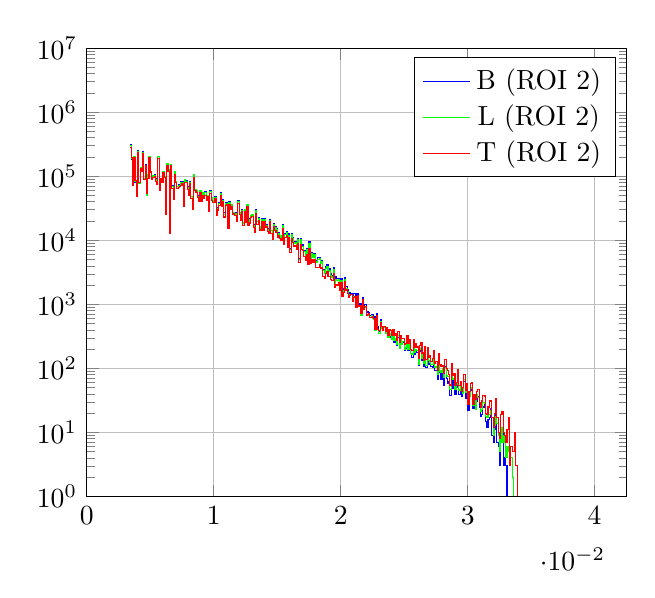
\begin{tikzpicture}

% Axis at [0.13 0.11 0.78 0.81]
\begin{semilogyaxis}[
xmajorgrids,
ymajorgrids,,
xmin=0, xmax=0.0425,
ymin=1, ymax=1e+007,
%title={ROI 2},
legend entries={%
	B (ROI 2),%
	L (ROI 2),%
	T (ROI 2)}
]

\addplot [
color=blue,
solid
]coordinates{
 (0.0034,0) (0.0034,312684) (0.0034,312684) (0.0035,312684) (0.0035,183652) (0.0035,183652) (0.0036,183652) (0.0036,72181) (0.0036,72181) (0.0037,72181) (0.0037,203079) (0.0037,203079) (0.0038,203079) (0.0038,81348) (0.0038,81348) (0.0039,81348) (0.0039,57975) (0.0039,57975) (0.004,57975) (0.004,251609) (0.004,251609) (0.0041,251609) (0.0041,77366) (0.0041,77366) (0.0042,77366) (0.0042,133350) (0.0042,133350) (0.0043,133350) (0.0043,122621) (0.0043,122621) (0.0044,122621) (0.0044,238856) (0.0044,238856) (0.0045,238856) (0.0045,91357) (0.0045,91357) (0.0046,91357) (0.0046,151741) (0.0046,151741) (0.0047,151741) (0.0047,50498) (0.0047,50498) (0.0048,50498) (0.0048,107490) (0.0048,107490) (0.0049,107490) (0.0049,202530) (0.0049,202530) (0.005,202530) (0.005,117031) (0.005,117031) (0.0051,117031) (0.0051,90436) (0.0051,90436) (0.0052,90436) (0.0052,102532) (0.0052,102532) (0.0053,102532) (0.0053,104440) (0.0053,104440) (0.0054,104440) (0.0054,92683) (0.0054,92683) (0.0055,92683) (0.0055,74215) (0.0055,74215) (0.0056,74215) (0.0056,202114) (0.0056,202114) (0.0057,202114) (0.0057,64957) (0.0057,64957) (0.0058,64957) (0.0058,92371) (0.0058,92371) (0.0059,92371) (0.0059,93414) (0.0059,93414) (0.006,93414) (0.006,117976) (0.006,117976) (0.0061,117976) (0.0061,100101) (0.0061,100101) (0.0062,100101) (0.0062,29238) (0.0062,29238) (0.0063,29238) (0.0063,156517) (0.0063,156517) (0.0064,156517) (0.0064,126816) (0.0064,126816) (0.0065,126816) (0.0065,15051) (0.0065,15051) (0.0066,15051) (0.0066,154257) (0.0066,154257) (0.0067,154257) (0.0067,70476) (0.0067,70476) (0.0068,70476) (0.0068,53144) (0.0068,53144) (0.0069,53144) (0.0069,118524) (0.0069,118524) (0.007,118524) (0.007,80872) (0.007,80872) (0.0071,80872) (0.0071,69883) (0.0071,69883) (0.0072,69883) (0.0072,73248) (0.0072,73248) (0.0073,73248) (0.0073,73056) (0.0073,73056) (0.0074,73056) (0.0074,81943) (0.0074,81943) (0.0075,81943) (0.0075,82336) (0.0075,82336) (0.0076,82336) (0.0076,34870) (0.0076,34870) (0.0077,34870) (0.0077,90165) (0.0077,90165) (0.0078,90165) (0.0078,85591) (0.0078,85591) (0.0079,85591) (0.0079,69000) (0.0079,69000) (0.008,69000) (0.008,53426) (0.008,53426) (0.0081,53426) (0.0081,82174) (0.0081,82174) (0.0082,82174) (0.0082,48163) (0.0082,48163) (0.0083,48163) (0.0083,32134) (0.0083,32134) (0.0084,32134) (0.0084,108019) (0.0084,108019) (0.0085,108019) (0.0085,62385) (0.0085,62385) (0.0086,62385) (0.0086,60667) (0.0086,60667) (0.0087,60667) (0.0087,49739) (0.0087,49739) (0.0088,49739) (0.0088,45786) (0.0088,45786) (0.0089,45786) (0.0089,60793) (0.0089,60793) (0.009,60793) (0.009,43213) (0.009,43213) (0.0091,43213) (0.0091,55618) (0.0091,55618) (0.0092,55618) (0.0092,47136) (0.0092,47136) (0.0093,47136) (0.0093,56912) (0.0093,56912) (0.0094,56912) (0.0094,46283) (0.0094,46283) (0.0095,46283) (0.0095,50548) (0.0095,50548) (0.0096,50548) (0.0096,29965) (0.0096,29965) (0.0097,29965) (0.0097,60117) (0.0097,60117) (0.0098,60117) (0.0098,46819) (0.0098,46819) (0.0099,46819) (0.0099,41596) (0.0099,41596) (0.01,41596) (0.01,42480) (0.01,42480) (0.0101,42480) (0.0101,47563) (0.0101,47563) (0.0102,47563) (0.0102,26856) (0.0102,26856) (0.0103,26856) (0.0103,32540) (0.0103,32540) (0.0104,32540) (0.0104,38902) (0.0104,38902) (0.0105,38902) (0.0105,55705) (0.0105,55705) (0.0106,55705) (0.0106,35274) (0.0106,35274) (0.0107,35274) (0.0107,42541) (0.0107,42541) (0.0108,42541) (0.0108,26751) (0.0108,26751) (0.0109,26751) (0.0109,38544) (0.0109,38544) (0.011,38544) (0.011,38598) (0.011,38598) (0.0111,38598) (0.0111,16569) (0.0111,16569) (0.0112,16569) (0.0112,40183) (0.0112,40183) (0.0113,40183) (0.0113,33424) (0.0113,33424) (0.0114,33424) (0.0114,36182) (0.0114,36182) (0.0115,36182) (0.0115,27454) (0.0115,27454) (0.0116,27454) (0.0116,25694) (0.0116,25694) (0.0117,25694) (0.0117,26744) (0.0117,26744) (0.0118,26744) (0.0118,22294) (0.0118,22294) (0.0119,22294) (0.0119,41553) (0.0119,41553) (0.012,41553) (0.012,27281) (0.012,27281) (0.0121,27281) (0.0121,21482) (0.0121,21482) (0.0122,21482) (0.0122,30080) (0.0122,30080) (0.0123,30080) (0.0123,19250) (0.0123,19250) (0.0124,19250) (0.0124,30286) (0.0124,30286) (0.0125,30286) (0.0125,21288) (0.0125,21288) (0.0126,21288) (0.0126,36326) (0.0126,36326) (0.0127,36326) (0.0127,18274) (0.0127,18274) (0.0128,18274) (0.0128,21641) (0.0128,21641) (0.0129,21641) (0.0129,24727) (0.0129,24727) (0.013,24727) (0.013,25295) (0.013,25295) (0.0131,25295) (0.0131,17520) (0.0131,17520) (0.0132,17520) (0.0132,14187) (0.0132,14187) (0.0133,14187) (0.0133,30537) (0.0133,30537) (0.0134,30537) (0.0134,19960) (0.0134,19960) (0.0135,19960) (0.0135,22371) (0.0135,22371) (0.0136,22371) (0.0136,15021) (0.0136,15021) (0.0137,15021) (0.0137,16606) (0.0137,16606) (0.0138,16606) (0.0138,21909) (0.0138,21909) (0.0139,21909) (0.0139,16093) (0.0139,16093) (0.014,16093) (0.014,21989) (0.014,21989) (0.0141,21989) (0.0141,17685) (0.0141,17685) (0.0142,17685) (0.0142,15267) (0.0142,15267) (0.0143,15267) (0.0143,14141) (0.0143,14141) (0.0144,14141) (0.0144,21333) (0.0144,21333) (0.0145,21333) (0.0145,14301) (0.0145,14301) (0.0146,14301) (0.0146,11654) (0.0146,11654) (0.0147,11654) (0.0147,18504) (0.0147,18504) (0.0148,18504) (0.0148,16269) (0.0148,16269) (0.0149,16269) (0.0149,15120) (0.0149,15120) (0.015,15120) (0.015,12028) (0.015,12028) (0.0151,12028) (0.0151,13099) (0.0151,13099) (0.0152,13099) (0.0152,11937) (0.0152,11937) (0.0153,11937) (0.0153,11650) (0.0153,11650) (0.0154,11650) (0.0154,17521) (0.0154,17521) (0.0155,17521) (0.0155,9461) (0.0155,9461) (0.0156,9461) (0.0156,12635) (0.0156,12635) (0.0157,12635) (0.0157,13566) (0.0157,13566) (0.0158,13566) (0.0158,8942) (0.0158,8942) (0.0159,8942) (0.0159,12681) (0.0159,12681) (0.016,12681) (0.016,7517) (0.016,7517) (0.0161,7517) (0.0161,12824) (0.0161,12824) (0.0162,12824) (0.0162,10928) (0.0162,10928) (0.0163,10928) (0.0163,9493) (0.0163,9493) (0.0164,9493) (0.0164,9593) (0.0164,9593) (0.0165,9593) (0.0165,8688) (0.0165,8688) (0.0166,8688) (0.0166,10838) (0.0166,10838) (0.0167,10838) (0.0167,5148) (0.0167,5148) (0.0168,5148) (0.0168,10691) (0.0168,10691) (0.0169,10691) (0.0169,8478) (0.0169,8478) (0.017,8478) (0.017,8447) (0.017,8447) (0.0171,8447) (0.0171,6831) (0.0171,6831) (0.0172,6831) (0.0172,6134) (0.0172,6134) (0.0173,6134) (0.0173,7402) (0.0173,7402) (0.0174,7402) (0.0174,5276) (0.0174,5276) (0.0175,5276) (0.0175,9481) (0.0175,9481) (0.0176,9481) (0.0176,5542) (0.0176,5542) (0.0177,5542) (0.0177,6368) (0.0177,6368) (0.0178,6368) (0.0178,5769) (0.0178,5769) (0.0179,5769) (0.0179,6167) (0.0179,6167) (0.018,6167) (0.018,4885) (0.018,4885) (0.0181,4885) (0.0181,4860) (0.0181,4860) (0.0182,4860) (0.0182,5387) (0.0182,5387) (0.0183,5387) (0.0183,5383) (0.0183,5383) (0.0184,5383) (0.0184,4555) (0.0184,4555) (0.0185,4555) (0.0185,4874) (0.0185,4874) (0.0186,4874) (0.0186,3464) (0.0186,3464) (0.0187,3464) (0.0187,3296) (0.0187,3296) (0.0188,3296) (0.0188,3855) (0.0188,3855) (0.0189,3855) (0.0189,4235) (0.0189,4235) (0.019,4235) (0.019,3457) (0.019,3457) (0.0191,3457) (0.0191,3605) (0.0191,3605) (0.0192,3605) (0.0192,3059) (0.0192,3059) (0.0193,3059) (0.0193,2844) (0.0193,2844) (0.0194,2844) (0.0194,3778) (0.0194,3778) (0.0195,3778) (0.0195,2331) (0.0195,2331) (0.0196,2331) (0.0196,2724) (0.0196,2724) (0.0197,2724) (0.0197,2562) (0.0197,2562) (0.0198,2562) (0.0198,2554) (0.0198,2554) (0.0199,2554) (0.0199,1978) (0.0199,1978) (0.02,1978) (0.02,2569) (0.02,2569) (0.0201,2569) (0.0201,1608) (0.0201,1608) (0.0202,1608) (0.0202,1749) (0.0202,1749) (0.0203,1749) (0.0203,2642) (0.0203,2642) (0.0204,2642) (0.0204,1903) (0.0204,1903) (0.0205,1903) (0.0205,1731) (0.0205,1731) (0.0206,1731) (0.0206,1422) (0.0206,1422) (0.0207,1422) (0.0207,1508) (0.0207,1508) (0.0208,1508) (0.0208,1491) (0.0208,1491) (0.0209,1491) (0.0209,1201) (0.0209,1201) (0.021,1201) (0.021,1460) (0.021,1460) (0.0211,1460) (0.0211,1457) (0.0211,1457) (0.0212,1457) (0.0212,1001) (0.0212,1001) (0.0213,1001) (0.0213,1449) (0.0213,1449) (0.0214,1449) (0.0214,1017) (0.0214,1017) (0.0215,1017) (0.0215,1014) (0.0215,1014) (0.0216,1014) (0.0216,754) (0.0216,754) (0.0217,754) (0.0217,1296) (0.0217,1296) (0.0218,1296) (0.0218,919) (0.0218,919) (0.0219,919) (0.0219,999) (0.0219,999) (0.022,999) (0.022,738) (0.022,738) (0.0221,738) (0.0221,763) (0.0221,763) (0.0222,763) (0.0222,755) (0.0222,755) (0.0223,755) (0.0223,674) (0.0223,674) (0.0224,674) (0.0224,699) (0.0224,699) (0.0225,699) (0.0225,683) (0.0225,683) (0.0226,683) (0.0226,641) (0.0226,641) (0.0227,641) (0.0227,431) (0.0227,431) (0.0228,431) (0.0228,707) (0.0228,707) (0.0229,707) (0.0229,447) (0.0229,447) (0.023,447) (0.023,374) (0.023,374) (0.0231,374) (0.0231,588) (0.0231,588) (0.0232,588) (0.0232,424) (0.0232,424) (0.0233,424) (0.0233,389) (0.0233,389) (0.0234,389) (0.0234,439) (0.0234,439) (0.0235,439) (0.0235,360) (0.0235,360) (0.0236,360) (0.0236,382) (0.0236,382) (0.0237,382) (0.0237,300) (0.0237,300) (0.0238,300) (0.0238,309) (0.0238,309) (0.0239,309) (0.0239,314) (0.0239,314) (0.024,314) (0.024,281) (0.024,281) (0.0241,281) (0.0241,328) (0.0241,328) (0.0242,328) (0.0242,256) (0.0242,256) (0.0243,256) (0.0243,284) (0.0243,284) (0.0244,284) (0.0244,227) (0.0244,227) (0.0245,227) (0.0245,303) (0.0245,303) (0.0246,303) (0.0246,211) (0.0246,211) (0.0247,211) (0.0247,264) (0.0247,264) (0.0248,264) (0.0248,244) (0.0248,244) (0.0249,244) (0.0249,250) (0.0249,250) (0.025,250) (0.025,191) (0.025,191) (0.0251,191) (0.0251,205) (0.0251,205) (0.0252,205) (0.0252,258) (0.0252,258) (0.0253,258) (0.0253,193) (0.0253,193) (0.0254,193) (0.0254,229) (0.0254,229) (0.0255,229) (0.0255,171) (0.0255,171) (0.0256,171) (0.0256,150) (0.0256,150) (0.0257,150) (0.0257,239) (0.0257,239) (0.0258,239) (0.0258,163) (0.0258,163) (0.0259,163) (0.0259,196) (0.0259,196) (0.026,196) (0.026,175) (0.026,175) (0.0261,175) (0.0261,111) (0.0261,111) (0.0262,111) (0.0262,186) (0.0262,186) (0.0263,186) (0.0263,192) (0.0263,192) (0.0264,192) (0.0264,134) (0.0264,134) (0.0265,134) (0.0265,109) (0.0265,109) (0.0266,109) (0.0266,172) (0.0266,172) (0.0267,172) (0.0267,104) (0.0267,104) (0.0268,104) (0.0268,167) (0.0268,167) (0.0269,167) (0.0269,115) (0.0269,115) (0.027,115) (0.027,117) (0.027,117) (0.0271,117) (0.0271,108) (0.0271,108) (0.0272,108) (0.0272,103) (0.0272,103) (0.0273,103) (0.0273,145) (0.0273,145) (0.0274,145) (0.0274,92) (0.0274,92) (0.0275,92) (0.0275,93) (0.0275,93) (0.0276,93) (0.0276,68) (0.0276,68) (0.0277,68) (0.0277,129) (0.0277,129) (0.0278,129) (0.0278,87) (0.0278,87) (0.0279,87) (0.0279,68) (0.0279,68) (0.028,68) (0.028,91) (0.028,91) (0.0281,91) (0.0281,55) (0.0281,55) (0.0282,55) (0.0282,108) (0.0282,108) (0.0283,108) (0.0283,69) (0.0283,69) (0.0284,69) (0.0284,59) (0.0284,59) (0.0285,59) (0.0285,63) (0.0285,63) (0.0286,63) (0.0286,38) (0.0286,38) (0.0287,38) (0.0287,100) (0.0287,100) (0.0288,100) (0.0288,48) (0.0288,48) (0.0289,48) (0.0289,65) (0.0289,65) (0.029,65) (0.029,39) (0.029,39) (0.0291,39) (0.0291,51) (0.0291,51) (0.0292,51) (0.0292,72) (0.0292,72) (0.0293,72) (0.0293,39) (0.0293,39) (0.0294,39) (0.0294,52) (0.0294,52) (0.0295,52) (0.0295,37) (0.0295,37) (0.0296,37) (0.0296,43) (0.0296,43) (0.0297,43) (0.0297,62) (0.0297,62) (0.0298,62) (0.0298,34) (0.0298,34) (0.0299,34) (0.0299,48) (0.0299,48) (0.03,48) (0.03,22) (0.03,22) (0.0301,22) (0.0301,36) (0.0301,36) (0.0302,36) (0.0302,46) (0.0302,46) (0.0303,46) (0.0303,46) (0.0303,46) (0.0304,46) (0.0304,24) (0.0304,24) (0.0305,24) (0.0305,30) (0.0305,30) (0.0306,30) (0.0306,24) (0.0306,24) (0.0307,24) (0.0307,30) (0.0307,30) (0.0308,30) (0.0308,36) (0.0308,36) (0.0309,36) (0.0309,25) (0.0309,25) (0.031,25) (0.031,18) (0.031,18) (0.0311,18) (0.0311,19) (0.0311,19) (0.0312,19) (0.0312,25) (0.0312,25) (0.0313,25) (0.0313,27) (0.0313,27) (0.0314,27) (0.0314,15) (0.0314,15) (0.0315,15) (0.0315,12) (0.0315,12) (0.0316,12) (0.0316,16) (0.0316,16) (0.0317,16) (0.0317,17) (0.0317,17) (0.0318,17) (0.0318,24) (0.0318,24) (0.0319,24) (0.0319,9) (0.0319,9) (0.032,9) (0.032,7) (0.032,7) (0.0321,7) (0.0321,11) (0.0321,11) (0.0322,11) (0.0322,20) (0.0322,20) (0.0323,20) (0.0323,7) (0.0323,7) (0.0324,7) (0.0324,6) (0.0324,6) (0.0325,6) (0.0325,3) (0.0325,3) (0.0326,3) (0.0326,8) (0.0326,8) (0.0327,8) (0.0327,11) (0.0327,11) (0.0328,11) (0.0328,3) (0.0328,3) (0.0329,3) (0.0329,4) (0.0329,4) (0.033,4) (0.033,3) (0.033,3) (0.0331,3) (0.0331,1)
};

\addplot [
color=green,
solid
]coordinates{
 (0.0034,0) (0.0034,306877) (0.0034,306877) (0.0035,306877) (0.0035,186332) (0.0035,186332) (0.0036,186332) (0.0036,72729) (0.0036,72729) (0.0037,72729) (0.0037,200153) (0.0037,200153) (0.0038,200153) (0.0038,82649) (0.0038,82649) (0.0039,82649) (0.0039,55923) (0.0039,55923) (0.004,55923) (0.004,247346) (0.004,247346) (0.0041,247346) (0.0041,77268) (0.0041,77268) (0.0042,77268) (0.0042,135430) (0.0042,135430) (0.0043,135430) (0.0043,121775) (0.0043,121775) (0.0044,121775) (0.0044,235153) (0.0044,235153) (0.0045,235153) (0.0045,90911) (0.0045,90911) (0.0046,90911) (0.0046,149549) (0.0046,149549) (0.0047,149549) (0.0047,50810) (0.0047,50810) (0.0048,50810) (0.0048,104509) (0.0048,104509) (0.0049,104509) (0.0049,202899) (0.0049,202899) (0.005,202899) (0.005,115960) (0.005,115960) (0.0051,115960) (0.0051,89976) (0.0051,89976) (0.0052,89976) (0.0052,101056) (0.0052,101056) (0.0053,101056) (0.0053,102429) (0.0053,102429) (0.0054,102429) (0.0054,89934) (0.0054,89934) (0.0055,89934) (0.0055,74882) (0.0055,74882) (0.0056,74882) (0.0056,200590) (0.0056,200590) (0.0057,200590) (0.0057,63428) (0.0057,63428) (0.0058,63428) (0.0058,92216) (0.0058,92216) (0.0059,92216) (0.0059,90374) (0.0059,90374) (0.006,90374) (0.006,116600) (0.006,116600) (0.0061,116600) (0.0061,99546) (0.0061,99546) (0.0062,99546) (0.0062,27520) (0.0062,27520) (0.0063,27520) (0.0063,155577) (0.0063,155577) (0.0064,155577) (0.0064,125212) (0.0064,125212) (0.0065,125212) (0.0065,14761) (0.0065,14761) (0.0066,14761) (0.0066,151976) (0.0066,151976) (0.0067,151976) (0.0067,69531) (0.0067,69531) (0.0068,69531) (0.0068,50527) (0.0068,50527) (0.0069,50527) (0.0069,116384) (0.0069,116384) (0.007,116384) (0.007,81560) (0.007,81560) (0.0071,81560) (0.0071,68601) (0.0071,68601) (0.0072,68601) (0.0072,72114) (0.0072,72114) (0.0073,72114) (0.0073,71899) (0.0073,71899) (0.0074,71899) (0.0074,79858) (0.0074,79858) (0.0075,79858) (0.0075,80683) (0.0075,80683) (0.0076,80683) (0.0076,34907) (0.0076,34907) (0.0077,34907) (0.0077,88788) (0.0077,88788) (0.0078,88788) (0.0078,84036) (0.0078,84036) (0.0079,84036) (0.0079,67309) (0.0079,67309) (0.008,67309) (0.008,52419) (0.008,52419) (0.0081,52419) (0.0081,80537) (0.0081,80537) (0.0082,80537) (0.0082,47692) (0.0082,47692) (0.0083,47692) (0.0083,31621) (0.0083,31621) (0.0084,31621) (0.0084,105376) (0.0084,105376) (0.0085,105376) (0.0085,61549) (0.0085,61549) (0.0086,61549) (0.0086,59629) (0.0086,59629) (0.0087,59629) (0.0087,48871) (0.0087,48871) (0.0088,48871) (0.0088,44244) (0.0088,44244) (0.0089,44244) (0.0089,59702) (0.0089,59702) (0.009,59702) (0.009,42276) (0.009,42276) (0.0091,42276) (0.0091,54692) (0.0091,54692) (0.0092,54692) (0.0092,46576) (0.0092,46576) (0.0093,46576) (0.0093,55168) (0.0093,55168) (0.0094,55168) (0.0094,45280) (0.0094,45280) (0.0095,45280) (0.0095,49785) (0.0095,49785) (0.0096,49785) (0.0096,29436) (0.0096,29436) (0.0097,29436) (0.0097,58609) (0.0097,58609) (0.0098,58609) (0.0098,45700) (0.0098,45700) (0.0099,45700) (0.0099,41446) (0.0099,41446) (0.01,41446) (0.01,40849) (0.01,40849) (0.0101,40849) (0.0101,46909) (0.0101,46909) (0.0102,46909) (0.0102,26434) (0.0102,26434) (0.0103,26434) (0.0103,31524) (0.0103,31524) (0.0104,31524) (0.0104,38003) (0.0104,38003) (0.0105,38003) (0.0105,54325) (0.0105,54325) (0.0106,54325) (0.0106,34654) (0.0106,34654) (0.0107,34654) (0.0107,42211) (0.0107,42211) (0.0108,42211) (0.0108,25650) (0.0108,25650) (0.0109,25650) (0.0109,37607) (0.0109,37607) (0.011,37607) (0.011,37726) (0.011,37726) (0.0111,37726) (0.0111,16151) (0.0111,16151) (0.0112,16151) (0.0112,39270) (0.0112,39270) (0.0113,39270) (0.0113,32589) (0.0113,32589) (0.0114,32589) (0.0114,35538) (0.0114,35538) (0.0115,35538) (0.0115,26774) (0.0115,26774) (0.0116,26774) (0.0116,25424) (0.0116,25424) (0.0117,25424) (0.0117,26003) (0.0117,26003) (0.0118,26003) (0.0118,21779) (0.0118,21779) (0.0119,21779) (0.0119,40321) (0.0119,40321) (0.012,40321) (0.012,26946) (0.012,26946) (0.0121,26946) (0.0121,21172) (0.0121,21172) (0.0122,21172) (0.0122,29568) (0.0122,29568) (0.0123,29568) (0.0123,18635) (0.0123,18635) (0.0124,18635) (0.0124,29685) (0.0124,29685) (0.0125,29685) (0.0125,20733) (0.0125,20733) (0.0126,20733) (0.0126,35629) (0.0126,35629) (0.0127,35629) (0.0127,18016) (0.0127,18016) (0.0128,18016) (0.0128,20729) (0.0128,20729) (0.0129,20729) (0.0129,24357) (0.0129,24357) (0.013,24357) (0.013,24835) (0.013,24835) (0.0131,24835) (0.0131,17137) (0.0131,17137) (0.0132,17137) (0.0132,13779) (0.0132,13779) (0.0133,13779) (0.0133,29537) (0.0133,29537) (0.0134,29537) (0.0134,19376) (0.0134,19376) (0.0135,19376) (0.0135,21972) (0.0135,21972) (0.0136,21972) (0.0136,14712) (0.0136,14712) (0.0137,14712) (0.0137,16189) (0.0137,16189) (0.0138,16189) (0.0138,21286) (0.0138,21286) (0.0139,21286) (0.0139,15513) (0.0139,15513) (0.014,15513) (0.014,21325) (0.014,21325) (0.0141,21325) (0.0141,17261) (0.0141,17261) (0.0142,17261) (0.0142,14687) (0.0142,14687) (0.0143,14687) (0.0143,14003) (0.0143,14003) (0.0144,14003) (0.0144,20587) (0.0144,20587) (0.0145,20587) (0.0145,14012) (0.0145,14012) (0.0146,14012) (0.0146,11303) (0.0146,11303) (0.0147,11303) (0.0147,17720) (0.0147,17720) (0.0148,17720) (0.0148,15753) (0.0148,15753) (0.0149,15753) (0.0149,14745) (0.0149,14745) (0.015,14745) (0.015,11626) (0.015,11626) (0.0151,11626) (0.0151,12693) (0.0151,12693) (0.0152,12693) (0.0152,11693) (0.0152,11693) (0.0153,11693) (0.0153,10983) (0.0153,10983) (0.0154,10983) (0.0154,16876) (0.0154,16876) (0.0155,16876) (0.0155,9224) (0.0155,9224) (0.0156,9224) (0.0156,12155) (0.0156,12155) (0.0157,12155) (0.0157,13054) (0.0157,13054) (0.0158,13054) (0.0158,8716) (0.0158,8716) (0.0159,8716) (0.0159,12019) (0.0159,12019) (0.016,12019) (0.016,7300) (0.016,7300) (0.0161,7300) (0.0161,12120) (0.0161,12120) (0.0162,12120) (0.0162,10590) (0.0162,10590) (0.0163,10590) (0.0163,9079) (0.0163,9079) (0.0164,9079) (0.0164,9296) (0.0164,9296) (0.0165,9296) (0.0165,8316) (0.0165,8316) (0.0166,8316) (0.0166,10320) (0.0166,10320) (0.0167,10320) (0.0167,5008) (0.0167,5008) (0.0168,5008) (0.0168,10092) (0.0168,10092) (0.0169,10092) (0.0169,8068) (0.0169,8068) (0.017,8068) (0.017,8064) (0.017,8064) (0.0171,8064) (0.0171,6619) (0.0171,6619) (0.0172,6619) (0.0172,5728) (0.0172,5728) (0.0173,5728) (0.0173,7221) (0.0173,7221) (0.0174,7221) (0.0174,5009) (0.0174,5009) (0.0175,5009) (0.0175,8991) (0.0175,8991) (0.0176,8991) (0.0176,5284) (0.0176,5284) (0.0177,5284) (0.0177,6225) (0.0177,6225) (0.0178,6225) (0.0178,5468) (0.0178,5468) (0.0179,5468) (0.0179,5912) (0.0179,5912) (0.018,5912) (0.018,4676) (0.018,4676) (0.0181,4676) (0.0181,4568) (0.0181,4568) (0.0182,4568) (0.0182,5089) (0.0182,5089) (0.0183,5089) (0.0183,5196) (0.0183,5196) (0.0184,5196) (0.0184,4374) (0.0184,4374) (0.0185,4374) (0.0185,4574) (0.0185,4574) (0.0186,4574) (0.0186,3332) (0.0186,3332) (0.0187,3332) (0.0187,3084) (0.0187,3084) (0.0188,3084) (0.0188,3675) (0.0188,3675) (0.0189,3675) (0.0189,3948) (0.0189,3948) (0.019,3948) (0.019,3264) (0.019,3264) (0.0191,3264) (0.0191,3335) (0.0191,3335) (0.0192,3335) (0.0192,2827) (0.0192,2827) (0.0193,2827) (0.0193,2675) (0.0193,2675) (0.0194,2675) (0.0194,3482) (0.0194,3482) (0.0195,3482) (0.0195,2146) (0.0195,2146) (0.0196,2146) (0.0196,2446) (0.0196,2446) (0.0197,2446) (0.0197,2341) (0.0197,2341) (0.0198,2341) (0.0198,2432) (0.0198,2432) (0.0199,2432) (0.0199,1821) (0.0199,1821) (0.02,1821) (0.02,2384) (0.02,2384) (0.0201,2384) (0.0201,1499) (0.0201,1499) (0.0202,1499) (0.0202,1639) (0.0202,1639) (0.0203,1639) (0.0203,2465) (0.0203,2465) (0.0204,2465) (0.0204,1794) (0.0204,1794) (0.0205,1794) (0.0205,1599) (0.0205,1599) (0.0206,1599) (0.0206,1333) (0.0206,1333) (0.0207,1333) (0.0207,1430) (0.0207,1430) (0.0208,1430) (0.0208,1431) (0.0208,1431) (0.0209,1431) (0.0209,1142) (0.0209,1142) (0.021,1142) (0.021,1331) (0.021,1331) (0.0211,1331) (0.0211,1340) (0.0211,1340) (0.0212,1340) (0.0212,918) (0.0212,918) (0.0213,918) (0.0213,1362) (0.0213,1362) (0.0214,1362) (0.0214,945) (0.0214,945) (0.0215,945) (0.0215,952) (0.0215,952) (0.0216,952) (0.0216,669) (0.0216,669) (0.0217,669) (0.0217,1167) (0.0217,1167) (0.0218,1167) (0.0218,877) (0.0218,877) (0.0219,877) (0.0219,904) (0.0219,904) (0.022,904) (0.022,667) (0.022,667) (0.0221,667) (0.0221,704) (0.0221,704) (0.0222,704) (0.0222,668) (0.0222,668) (0.0223,668) (0.0223,619) (0.0223,619) (0.0224,619) (0.0224,666) (0.0224,666) (0.0225,666) (0.0225,603) (0.0225,603) (0.0226,603) (0.0226,584) (0.0226,584) (0.0227,584) (0.0227,394) (0.0227,394) (0.0228,394) (0.0228,670) (0.0228,670) (0.0229,670) (0.0229,408) (0.0229,408) (0.023,408) (0.023,352) (0.023,352) (0.0231,352) (0.0231,535) (0.0231,535) (0.0232,535) (0.0232,421) (0.0232,421) (0.0233,421) (0.0233,399) (0.0233,399) (0.0234,399) (0.0234,437) (0.0234,437) (0.0235,437) (0.0235,345) (0.0235,345) (0.0236,345) (0.0236,390) (0.0236,390) (0.0237,390) (0.0237,299) (0.0237,299) (0.0238,299) (0.0238,347) (0.0238,347) (0.0239,347) (0.0239,325) (0.0239,325) (0.024,325) (0.024,284) (0.024,284) (0.0241,284) (0.0241,341) (0.0241,341) (0.0242,341) (0.0242,274) (0.0242,274) (0.0243,274) (0.0243,288) (0.0243,288) (0.0244,288) (0.0244,238) (0.0244,238) (0.0245,238) (0.0245,327) (0.0245,327) (0.0246,327) (0.0246,206) (0.0246,206) (0.0247,206) (0.0247,303) (0.0247,303) (0.0248,303) (0.0248,238) (0.0248,238) (0.0249,238) (0.0249,264) (0.0249,264) (0.025,264) (0.025,195) (0.025,195) (0.0251,195) (0.0251,214) (0.0251,214) (0.0252,214) (0.0252,277) (0.0252,277) (0.0253,277) (0.0253,200) (0.0253,200) (0.0254,200) (0.0254,237) (0.0254,237) (0.0255,237) (0.0255,172) (0.0255,172) (0.0256,172) (0.0256,168) (0.0256,168) (0.0257,168) (0.0257,242) (0.0257,242) (0.0258,242) (0.0258,180) (0.0258,180) (0.0259,180) (0.0259,197) (0.0259,197) (0.026,197) (0.026,193) (0.026,193) (0.0261,193) (0.0261,114) (0.0261,114) (0.0262,114) (0.0262,196) (0.0262,196) (0.0263,196) (0.0263,207) (0.0263,207) (0.0264,207) (0.0264,143) (0.0264,143) (0.0265,143) (0.0265,120) (0.0265,120) (0.0266,120) (0.0266,181) (0.0266,181) (0.0267,181) (0.0267,112) (0.0267,112) (0.0268,112) (0.0268,174) (0.0268,174) (0.0269,174) (0.0269,133) (0.0269,133) (0.027,133) (0.027,123) (0.027,123) (0.0271,123) (0.0271,116) (0.0271,116) (0.0272,116) (0.0272,116) (0.0272,116) (0.0273,116) (0.0273,148) (0.0273,148) (0.0274,148) (0.0274,105) (0.0274,105) (0.0275,105) (0.0275,105) (0.0275,105) (0.0276,105) (0.0276,80) (0.0276,80) (0.0277,80) (0.0277,135) (0.0277,135) (0.0278,135) (0.0278,91) (0.0278,91) (0.0279,91) (0.0279,87) (0.0279,87) (0.028,87) (0.028,101) (0.028,101) (0.0281,101) (0.0281,73) (0.0281,73) (0.0282,73) (0.0282,104) (0.0282,104) (0.0283,104) (0.0283,76) (0.0283,76) (0.0284,76) (0.0284,74) (0.0284,74) (0.0285,74) (0.0285,74) (0.0285,74) (0.0286,74) (0.0286,47) (0.0286,47) (0.0287,47) (0.0287,87) (0.0287,87) (0.0288,87) (0.0288,67) (0.0288,67) (0.0289,67) (0.0289,70) (0.0289,70) (0.029,70) (0.029,47) (0.029,47) (0.0291,47) (0.0291,57) (0.0291,57) (0.0292,57) (0.0292,71) (0.0292,71) (0.0293,71) (0.0293,46) (0.0293,46) (0.0294,46) (0.0294,59) (0.0294,59) (0.0295,59) (0.0295,47) (0.0295,47) (0.0296,47) (0.0296,41) (0.0296,41) (0.0297,41) (0.0297,67) (0.0297,67) (0.0298,67) (0.0298,42) (0.0298,42) (0.0299,42) (0.0299,50) (0.0299,50) (0.03,50) (0.03,29) (0.03,29) (0.0301,29) (0.0301,37) (0.0301,37) (0.0302,37) (0.0302,49) (0.0302,49) (0.0303,49) (0.0303,51) (0.0303,51) (0.0304,51) (0.0304,26) (0.0304,26) (0.0305,26) (0.0305,36) (0.0305,36) (0.0306,36) (0.0306,23) (0.0306,23) (0.0307,23) (0.0307,39) (0.0307,39) (0.0308,39) (0.0308,35) (0.0308,35) (0.0309,35) (0.0309,29) (0.0309,29) (0.031,29) (0.031,21) (0.031,21) (0.0311,21) (0.0311,23) (0.0311,23) (0.0312,23) (0.0312,29) (0.0312,29) (0.0313,29) (0.0313,28) (0.0313,28) (0.0314,28) (0.0314,18) (0.0314,18) (0.0315,18) (0.0315,17) (0.0315,17) (0.0316,17) (0.0316,19) (0.0316,19) (0.0317,19) (0.0317,19) (0.0317,19) (0.0318,19) (0.0318,22) (0.0318,22) (0.0319,22) (0.0319,17) (0.0319,17) (0.032,17) (0.032,9) (0.032,9) (0.0321,9) (0.0321,13) (0.0321,13) (0.0322,13) (0.0322,18) (0.0322,18) (0.0323,18) (0.0323,14) (0.0323,14) (0.0324,14) (0.0324,9) (0.0324,9) (0.0325,9) (0.0325,5) (0.0325,5) (0.0326,5) (0.0326,12) (0.0326,12) (0.0327,12) (0.0327,7) (0.0327,7) (0.0328,7) (0.0328,9) (0.0328,9) (0.0329,9) (0.0329,7) (0.0329,7) (0.033,7) (0.033,4) (0.033,4) (0.0331,4) (0.0331,6) (0.0331,6) (0.0332,6) (0.0332,5) (0.0332,5) (0.0333,5) (0.0333,3) (0.0333,3) (0.0334,3) (0.0334,4) (0.0334,4) (0.0335,4) (0.0335,2) (0.0335,2) (0.0336,2) (0.0336,1)
};

\addplot [
color=red,
solid
]coordinates{
 (0.0034,0) (0.0034,285131) (0.0034,285131) (0.0035,285131) (0.0035,194800) (0.0035,194800) (0.0036,194800) (0.0036,72119) (0.0036,72119) (0.0037,72119) (0.0037,194996) (0.0037,194996) (0.0038,194996) (0.0038,87049) (0.0038,87049) (0.0039,87049) (0.0039,49115) (0.0039,49115) (0.004,49115) (0.004,235154) (0.004,235154) (0.0041,235154) (0.0041,79761) (0.0041,79761) (0.0042,79761) (0.0042,131809) (0.0042,131809) (0.0043,131809) (0.0043,118571) (0.0043,118571) (0.0044,118571) (0.0044,224443) (0.0044,224443) (0.0045,224443) (0.0045,90297) (0.0045,90297) (0.0046,90297) (0.0046,144381) (0.0046,144381) (0.0047,144381) (0.0047,52937) (0.0047,52937) (0.0048,52937) (0.0048,92686) (0.0048,92686) (0.0049,92686) (0.0049,193870) (0.0049,193870) (0.005,193870) (0.005,116363) (0.005,116363) (0.0051,116363) (0.0051,87883) (0.0051,87883) (0.0052,87883) (0.0052,94827) (0.0052,94827) (0.0053,94827) (0.0053,98715) (0.0053,98715) (0.0054,98715) (0.0054,81631) (0.0054,81631) (0.0055,81631) (0.0055,75132) (0.0055,75132) (0.0056,75132) (0.0056,189215) (0.0056,189215) (0.0057,189215) (0.0057,60645) (0.0057,60645) (0.0058,60645) (0.0058,91178) (0.0058,91178) (0.0059,91178) (0.0059,81288) (0.0059,81288) (0.006,81288) (0.006,113102) (0.006,113102) (0.0061,113102) (0.0061,95931) (0.0061,95931) (0.0062,95931) (0.0062,25217) (0.0062,25217) (0.0063,25217) (0.0063,144755) (0.0063,144755) (0.0064,144755) (0.0064,119814) (0.0064,119814) (0.0065,119814) (0.0065,12988) (0.0065,12988) (0.0066,12988) (0.0066,147960) (0.0066,147960) (0.0067,147960) (0.0067,64841) (0.0067,64841) (0.0068,64841) (0.0068,44177) (0.0068,44177) (0.0069,44177) (0.0069,106688) (0.0069,106688) (0.007,106688) (0.007,80323) (0.007,80323) (0.0071,80323) (0.0071,65279) (0.0071,65279) (0.0072,65279) (0.0072,67123) (0.0072,67123) (0.0073,67123) (0.0073,70082) (0.0073,70082) (0.0074,70082) (0.0074,71918) (0.0074,71918) (0.0075,71918) (0.0075,77536) (0.0075,77536) (0.0076,77536) (0.0076,33780) (0.0076,33780) (0.0077,33780) (0.0077,80727) (0.0077,80727) (0.0078,80727) (0.0078,80397) (0.0078,80397) (0.0079,80397) (0.0079,61598) (0.0079,61598) (0.008,61598) (0.008,50010) (0.008,50010) (0.0081,50010) (0.0081,76079) (0.0081,76079) (0.0082,76079) (0.0082,45457) (0.0082,45457) (0.0083,45457) (0.0083,29935) (0.0083,29935) (0.0084,29935) (0.0084,95253) (0.0084,95253) (0.0085,95253) (0.0085,59372) (0.0085,59372) (0.0086,59372) (0.0086,56652) (0.0086,56652) (0.0087,56652) (0.0087,46101) (0.0087,46101) (0.0088,46101) (0.0088,40536) (0.0088,40536) (0.0089,40536) (0.0089,55090) (0.0089,55090) (0.009,55090) (0.009,39760) (0.009,39760) (0.0091,39760) (0.0091,50313) (0.0091,50313) (0.0092,50313) (0.0092,45262) (0.0092,45262) (0.0093,45262) (0.0093,50780) (0.0093,50780) (0.0094,50780) (0.0094,41810) (0.0094,41810) (0.0095,41810) (0.0095,47488) (0.0095,47488) (0.0096,47488) (0.0096,28039) (0.0096,28039) (0.0097,28039) (0.0097,54492) (0.0097,54492) (0.0098,54492) (0.0098,41576) (0.0098,41576) (0.0099,41576) (0.0099,38900) (0.0099,38900) (0.01,38900) (0.01,38648) (0.01,38648) (0.0101,38648) (0.0101,44769) (0.0101,44769) (0.0102,44769) (0.0102,24587) (0.0102,24587) (0.0103,24587) (0.0103,29665) (0.0103,29665) (0.0104,29665) (0.0104,35369) (0.0104,35369) (0.0105,35369) (0.0105,49755) (0.0105,49755) (0.0106,49755) (0.0106,33236) (0.0106,33236) (0.0107,33236) (0.0107,40596) (0.0107,40596) (0.0108,40596) (0.0108,23119) (0.0108,23119) (0.0109,23119) (0.0109,35320) (0.0109,35320) (0.011,35320) (0.011,36367) (0.011,36367) (0.0111,36367) (0.0111,15242) (0.0111,15242) (0.0112,15242) (0.0112,35527) (0.0112,35527) (0.0113,35527) (0.0113,30556) (0.0113,30556) (0.0114,30556) (0.0114,33313) (0.0114,33313) (0.0115,33313) (0.0115,25767) (0.0115,25767) (0.0116,25767) (0.0116,24223) (0.0116,24223) (0.0117,24223) (0.0117,24463) (0.0117,24463) (0.0118,24463) (0.0118,20049) (0.0118,20049) (0.0119,20049) (0.0119,37178) (0.0119,37178) (0.012,37178) (0.012,25496) (0.012,25496) (0.0121,25496) (0.0121,20191) (0.0121,20191) (0.0122,20191) (0.0122,27732) (0.0122,27732) (0.0123,27732) (0.0123,16941) (0.0123,16941) (0.0124,16941) (0.0124,28183) (0.0124,28183) (0.0125,28183) (0.0125,19086) (0.0125,19086) (0.0126,19086) (0.0126,33317) (0.0126,33317) (0.0127,33317) (0.0127,17002) (0.0127,17002) (0.0128,17002) (0.0128,18625) (0.0128,18625) (0.0129,18625) (0.0129,22955) (0.0129,22955) (0.013,22955) (0.013,23289) (0.013,23289) (0.0131,23289) (0.0131,15955) (0.0131,15955) (0.0132,15955) (0.0132,13147) (0.0132,13147) (0.0133,13147) (0.0133,26527) (0.0133,26527) (0.0134,26527) (0.0134,17817) (0.0134,17817) (0.0135,17817) (0.0135,20686) (0.0135,20686) (0.0136,20686) (0.0136,14011) (0.0136,14011) (0.0137,14011) (0.0137,14467) (0.0137,14467) (0.0138,14467) (0.0138,19823) (0.0138,19823) (0.0139,19823) (0.0139,14399) (0.0139,14399) (0.014,14399) (0.014,19457) (0.014,19457) (0.0141,19457) (0.0141,16114) (0.0141,16114) (0.0142,16114) (0.0142,13799) (0.0142,13799) (0.0143,13799) (0.0143,12583) (0.0143,12583) (0.0144,12583) (0.0144,19302) (0.0144,19302) (0.0145,19302) (0.0145,12926) (0.0145,12926) (0.0146,12926) (0.0146,10330) (0.0146,10330) (0.0147,10330) (0.0147,16228) (0.0147,16228) (0.0148,16228) (0.0148,14403) (0.0148,14403) (0.0149,14403) (0.0149,13399) (0.0149,13399) (0.015,13399) (0.015,11018) (0.015,11018) (0.0151,11018) (0.0151,11651) (0.0151,11651) (0.0152,11651) (0.0152,10579) (0.0152,10579) (0.0153,10579) (0.0153,9820) (0.0153,9820) (0.0154,9820) (0.0154,15237) (0.0154,15237) (0.0155,15237) (0.0155,8463) (0.0155,8463) (0.0156,8463) (0.0156,11058) (0.0156,11058) (0.0157,11058) (0.0157,11745) (0.0157,11745) (0.0158,11745) (0.0158,7638) (0.0158,7638) (0.0159,7638) (0.0159,10852) (0.0159,10852) (0.016,10852) (0.016,6548) (0.016,6548) (0.0161,6548) (0.0161,10677) (0.0161,10677) (0.0162,10677) (0.0162,9300) (0.0162,9300) (0.0163,9300) (0.0163,7938) (0.0163,7938) (0.0164,7938) (0.0164,8310) (0.0164,8310) (0.0165,8310) (0.0165,7159) (0.0165,7159) (0.0166,7159) (0.0166,9043) (0.0166,9043) (0.0167,9043) (0.0167,4445) (0.0167,4445) (0.0168,4445) (0.0168,8456) (0.0168,8456) (0.0169,8456) (0.0169,7130) (0.0169,7130) (0.017,7130) (0.017,6949) (0.017,6949) (0.0171,6949) (0.0171,5573) (0.0171,5573) (0.0172,5573) (0.0172,4830) (0.0172,4830) (0.0173,4830) (0.0173,6084) (0.0173,6084) (0.0174,6084) (0.0174,4192) (0.0174,4192) (0.0175,4192) (0.0175,7446) (0.0175,7446) (0.0176,7446) (0.0176,4399) (0.0176,4399) (0.0177,4399) (0.0177,5049) (0.0177,5049) (0.0178,5049) (0.0178,4523) (0.0178,4523) (0.0179,4523) (0.0179,4954) (0.0179,4954) (0.018,4954) (0.018,3783) (0.018,3783) (0.0181,3783) (0.0181,3815) (0.0181,3815) (0.0182,3815) (0.0182,3817) (0.0182,3817) (0.0183,3817) (0.0183,4204) (0.0183,4204) (0.0184,4204) (0.0184,3573) (0.0184,3573) (0.0185,3573) (0.0185,3817) (0.0185,3817) (0.0186,3817) (0.0186,2701) (0.0186,2701) (0.0187,2701) (0.0187,2550) (0.0187,2550) (0.0188,2550) (0.0188,3044) (0.0188,3044) (0.0189,3044) (0.0189,3208) (0.0189,3208) (0.019,3208) (0.019,2684) (0.019,2684) (0.0191,2684) (0.0191,2751) (0.0191,2751) (0.0192,2751) (0.0192,2451) (0.0192,2451) (0.0193,2451) (0.0193,2321) (0.0193,2321) (0.0194,2321) (0.0194,2997) (0.0194,2997) (0.0195,2997) (0.0195,1867) (0.0195,1867) (0.0196,1867) (0.0196,2028) (0.0196,2028) (0.0197,2028) (0.0197,2005) (0.0197,2005) (0.0198,2005) (0.0198,2215) (0.0198,2215) (0.0199,2215) (0.0199,1662) (0.0199,1662) (0.02,1662) (0.02,2173) (0.02,2173) (0.0201,2173) (0.0201,1349) (0.0201,1349) (0.0202,1349) (0.0202,1516) (0.0202,1516) (0.0203,1516) (0.0203,2251) (0.0203,2251) (0.0204,2251) (0.0204,1677) (0.0204,1677) (0.0205,1677) (0.0205,1482) (0.0205,1482) (0.0206,1482) (0.0206,1277) (0.0206,1277) (0.0207,1277) (0.0207,1383) (0.0207,1383) (0.0208,1383) (0.0208,1408) (0.0208,1408) (0.0209,1408) (0.0209,1111) (0.0209,1111) (0.021,1111) (0.021,1275) (0.021,1275) (0.0211,1275) (0.0211,1325) (0.0211,1325) (0.0212,1325) (0.0212,887) (0.0212,887) (0.0213,887) (0.0213,1363) (0.0213,1363) (0.0214,1363) (0.0214,932) (0.0214,932) (0.0215,932) (0.0215,943) (0.0215,943) (0.0216,943) (0.0216,720) (0.0216,720) (0.0217,720) (0.0217,1190) (0.0217,1190) (0.0218,1190) (0.0218,819) (0.0218,819) (0.0219,819) (0.0219,916) (0.0219,916) (0.022,916) (0.022,681) (0.022,681) (0.0221,681) (0.0221,704) (0.0221,704) (0.0222,704) (0.0222,719) (0.0222,719) (0.0223,719) (0.0223,624) (0.0223,624) (0.0224,624) (0.0224,623) (0.0224,623) (0.0225,623) (0.0225,641) (0.0225,641) (0.0226,641) (0.0226,600) (0.0226,600) (0.0227,600) (0.0227,399) (0.0227,399) (0.0228,399) (0.0228,669) (0.0228,669) (0.0229,669) (0.0229,411) (0.0229,411) (0.023,411) (0.023,391) (0.023,391) (0.0231,391) (0.0231,513) (0.0231,513) (0.0232,513) (0.0232,453) (0.0232,453) (0.0233,453) (0.0233,396) (0.0233,396) (0.0234,396) (0.0234,453) (0.0234,453) (0.0235,453) (0.0235,378) (0.0235,378) (0.0236,378) (0.0236,431) (0.0236,431) (0.0237,431) (0.0237,332) (0.0237,332) (0.0238,332) (0.0238,402) (0.0238,402) (0.0239,402) (0.0239,391) (0.0239,391) (0.024,391) (0.024,322) (0.024,322) (0.0241,322) (0.0241,410) (0.0241,410) (0.0242,410) (0.0242,324) (0.0242,324) (0.0243,324) (0.0243,347) (0.0243,347) (0.0244,347) (0.0244,277) (0.0244,277) (0.0245,277) (0.0245,377) (0.0245,377) (0.0246,377) (0.0246,258) (0.0246,258) (0.0247,258) (0.0247,325) (0.0247,325) (0.0248,325) (0.0248,295) (0.0248,295) (0.0249,295) (0.0249,296) (0.0249,296) (0.025,296) (0.025,233) (0.025,233) (0.0251,233) (0.0251,248) (0.0251,248) (0.0252,248) (0.0252,331) (0.0252,331) (0.0253,331) (0.0253,247) (0.0253,247) (0.0254,247) (0.0254,277) (0.0254,277) (0.0255,277) (0.0255,198) (0.0255,198) (0.0256,198) (0.0256,191) (0.0256,191) (0.0257,191) (0.0257,284) (0.0257,284) (0.0258,284) (0.0258,213) (0.0258,213) (0.0259,213) (0.0259,248) (0.0259,248) (0.026,248) (0.026,216) (0.026,216) (0.0261,216) (0.0261,144) (0.0261,144) (0.0262,144) (0.0262,227) (0.0262,227) (0.0263,227) (0.0263,250) (0.0263,250) (0.0264,250) (0.0264,174) (0.0264,174) (0.0265,174) (0.0265,131) (0.0265,131) (0.0266,131) (0.0266,218) (0.0266,218) (0.0267,218) (0.0267,138) (0.0267,138) (0.0268,138) (0.0268,213) (0.0268,213) (0.0269,213) (0.0269,149) (0.0269,149) (0.027,149) (0.027,159) (0.027,159) (0.0271,159) (0.0271,127) (0.0271,127) (0.0272,127) (0.0272,144) (0.0272,144) (0.0273,144) (0.0273,187) (0.0273,187) (0.0274,187) (0.0274,121) (0.0274,121) (0.0275,121) (0.0275,130) (0.0275,130) (0.0276,130) (0.0276,94) (0.0276,94) (0.0277,94) (0.0277,170) (0.0277,170) (0.0278,170) (0.0278,116) (0.0278,116) (0.0279,116) (0.0279,106) (0.0279,106) (0.028,106) (0.028,109) (0.028,109) (0.0281,109) (0.0281,83) (0.0281,83) (0.0282,83) (0.0282,138) (0.0282,138) (0.0283,138) (0.0283,101) (0.0283,101) (0.0284,101) (0.0284,93) (0.0284,93) (0.0285,93) (0.0285,80) (0.0285,80) (0.0286,80) (0.0286,55) (0.0286,55) (0.0287,55) (0.0287,119) (0.0287,119) (0.0288,119) (0.0288,77) (0.0288,77) (0.0289,77) (0.0289,82) (0.0289,82) (0.029,82) (0.029,54) (0.029,54) (0.0291,54) (0.0291,61) (0.0291,61) (0.0292,61) (0.0292,96) (0.0292,96) (0.0293,96) (0.0293,54) (0.0293,54) (0.0294,54) (0.0294,62) (0.0294,62) (0.0295,62) (0.0295,44) (0.0295,44) (0.0296,44) (0.0296,50) (0.0296,50) (0.0297,50) (0.0297,80) (0.0297,80) (0.0298,80) (0.0298,45) (0.0298,45) (0.0299,45) (0.0299,57) (0.0299,57) (0.03,57) (0.03,27) (0.03,27) (0.0301,27) (0.0301,43) (0.0301,43) (0.0302,43) (0.0302,59) (0.0302,59) (0.0303,59) (0.0303,61) (0.0303,61) (0.0304,61) (0.0304,27) (0.0304,27) (0.0305,27) (0.0305,39) (0.0305,39) (0.0306,39) (0.0306,33) (0.0306,33) (0.0307,33) (0.0307,43) (0.0307,43) (0.0308,43) (0.0308,47) (0.0308,47) (0.0309,47) (0.0309,29) (0.0309,29) (0.031,29) (0.031,25) (0.031,25) (0.0311,25) (0.0311,31) (0.0311,31) (0.0312,31) (0.0312,38) (0.0312,38) (0.0313,38) (0.0313,37) (0.0313,37) (0.0314,37) (0.0314,20) (0.0314,20) (0.0315,20) (0.0315,19) (0.0315,19) (0.0316,19) (0.0316,25) (0.0316,25) (0.0317,25) (0.0317,31) (0.0317,31) (0.0318,31) (0.0318,31) (0.0318,31) (0.0319,31) (0.0319,17) (0.0319,17) (0.032,17) (0.032,12) (0.032,12) (0.0321,12) (0.0321,20) (0.0321,20) (0.0322,20) (0.0322,34) (0.0322,34) (0.0323,34) (0.0323,17) (0.0323,17) (0.0324,17) (0.0324,10) (0.0324,10) (0.0325,10) (0.0325,8) (0.0325,8) (0.0326,8) (0.0326,19) (0.0326,19) (0.0327,19) (0.0327,21) (0.0327,21) (0.0328,21) (0.0328,10) (0.0328,10) (0.0329,10) (0.0329,9) (0.0329,9) (0.033,9) (0.033,7) (0.033,7) (0.0331,7) (0.0331,11) (0.0331,11) (0.0332,11) (0.0332,17) (0.0332,17) (0.0333,17) (0.0333,3) (0.0333,3) (0.0334,3) (0.0334,6) (0.0334,6) (0.0335,6) (0.0335,5) (0.0335,5) (0.0336,5) (0.0336,5) (0.0336,5) (0.0337,5) (0.0337,10) (0.0337,10) (0.0338,10) (0.0338,3) (0.0338,3) (0.0339,3) (0.0339,1)
};

\end{semilogyaxis}

\end{tikzpicture}
%%%%%%%%%%%%
%\end{preview}
%\end{document}\\%
		%\documentclass{article}
%\usepackage{tikz,pgfplots}
%\usepackage[pdftex,active,tightpage]{preview}
%\begin{document}
%\begin{preview}
%%%%%%%%%%%%
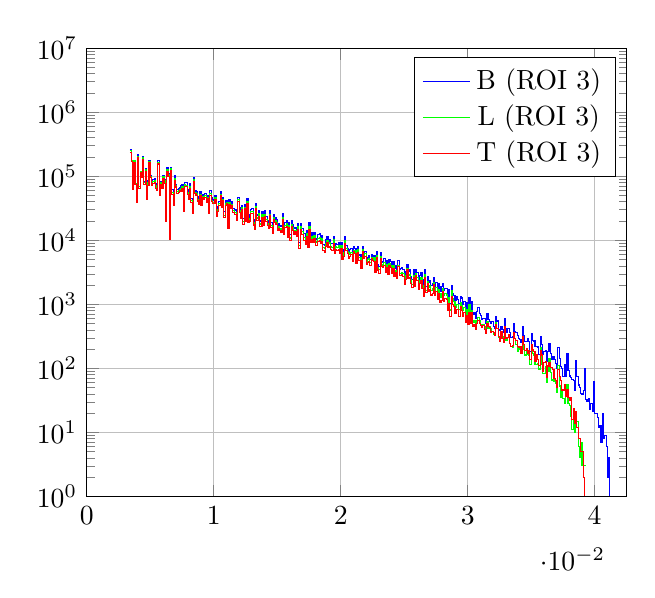
\begin{tikzpicture}

% Axis at [0.13 0.11 0.78 0.81]
\begin{semilogyaxis}[
xmajorgrids,
ymajorgrids,
xmin=0, xmax=0.0425,
ymin=1, ymax=1e+007,
%title={ROI 3},
legend entries={%
	B (ROI 3),%
	L (ROI 3),%
	T (ROI 3)}
]

\addplot [
color=blue,
solid
]coordinates{
 (0.0034,0) (0.0034,261785) (0.0034,261785) (0.0035,261785) (0.0035,171515) (0.0035,171515) (0.0036,171515) (0.0036,64140) (0.0036,64140) (0.0037,64140) (0.0037,178393) (0.0037,178393) (0.0038,178393) (0.0038,75348) (0.0038,75348) (0.0039,75348) (0.0039,46382) (0.0039,46382) (0.004,46382) (0.004,215725) (0.004,215725) (0.0041,215725) (0.0041,70020) (0.0041,70020) (0.0042,70020) (0.0042,119131) (0.0042,119131) (0.0043,119131) (0.0043,106518) (0.0043,106518) (0.0044,106518) (0.0044,205464) (0.0044,205464) (0.0045,205464) (0.0045,81381) (0.0045,81381) (0.0046,81381) (0.0046,132090) (0.0046,132090) (0.0047,132090) (0.0047,46500) (0.0047,46500) (0.0048,46500) (0.0048,86882) (0.0048,86882) (0.0049,86882) (0.0049,177449) (0.0049,177449) (0.005,177449) (0.005,104384) (0.005,104384) (0.0051,104384) (0.0051,79704) (0.0051,79704) (0.0052,79704) (0.0052,88134) (0.0052,88134) (0.0053,88134) (0.0053,91390) (0.0053,91390) (0.0054,91390) (0.0054,76156) (0.0054,76156) (0.0055,76156) (0.0055,67375) (0.0055,67375) (0.0056,67375) (0.0056,175138) (0.0056,175138) (0.0057,175138) (0.0057,56787) (0.0057,56787) (0.0058,56787) (0.0058,83486) (0.0058,83486) (0.0059,83486) (0.0059,76929) (0.0059,76929) (0.006,76929) (0.006,104060) (0.006,104060) (0.0061,104060) (0.0061,89587) (0.0061,89587) (0.0062,89587) (0.0062,24366) (0.0062,24366) (0.0063,24366) (0.0063,135688) (0.0063,135688) (0.0064,135688) (0.0064,111384) (0.0064,111384) (0.0065,111384) (0.0065,12855) (0.0065,12855) (0.0066,12855) (0.0066,138682) (0.0066,138682) (0.0067,138682) (0.0067,61809) (0.0067,61809) (0.0068,61809) (0.0068,44046) (0.0068,44046) (0.0069,44046) (0.0069,101518) (0.0069,101518) (0.007,101518) (0.007,75075) (0.007,75075) (0.0071,75075) (0.0071,62390) (0.0071,62390) (0.0072,62390) (0.0072,64998) (0.0072,64998) (0.0073,64998) (0.0073,67452) (0.0073,67452) (0.0074,67452) (0.0074,70334) (0.0074,70334) (0.0075,70334) (0.0075,75439) (0.0075,75439) (0.0076,75439) (0.0076,32535) (0.0076,32535) (0.0077,32535) (0.0077,79527) (0.0077,79527) (0.0078,79527) (0.0078,79109) (0.0078,79109) (0.0079,79109) (0.0079,61326) (0.0079,61326) (0.008,61326) (0.008,49543) (0.008,49543) (0.0081,49543) (0.0081,76006) (0.0081,76006) (0.0082,76006) (0.0082,45404) (0.0082,45404) (0.0083,45404) (0.0083,30199) (0.0083,30199) (0.0084,30199) (0.0084,96990) (0.0084,96990) (0.0085,96990) (0.0085,59335) (0.0085,59335) (0.0086,59335) (0.0086,57673) (0.0086,57673) (0.0087,57673) (0.0087,47603) (0.0087,47603) (0.0088,47603) (0.0088,42628) (0.0088,42628) (0.0089,42628) (0.0089,56988) (0.0089,56988) (0.009,56988) (0.009,41656) (0.009,41656) (0.0091,41656) (0.0091,52682) (0.0091,52682) (0.0092,52682) (0.0092,47187) (0.0092,47187) (0.0093,47187) (0.0093,54647) (0.0093,54647) (0.0094,54647) (0.0094,44404) (0.0094,44404) (0.0095,44404) (0.0095,50761) (0.0095,50761) (0.0096,50761) (0.0096,30337) (0.0096,30337) (0.0097,30337) (0.0097,59373) (0.0097,59373) (0.0098,59373) (0.0098,46057) (0.0098,46057) (0.0099,46057) (0.0099,42555) (0.0099,42555) (0.01,42555) (0.01,43013) (0.01,43013) (0.0101,43013) (0.0101,49493) (0.0101,49493) (0.0102,49493) (0.0102,27597) (0.0102,27597) (0.0103,27597) (0.0103,33162) (0.0103,33162) (0.0104,33162) (0.0104,40629) (0.0104,40629) (0.0105,40629) (0.0105,57212) (0.0105,57212) (0.0106,57212) (0.0106,37835) (0.0106,37835) (0.0107,37835) (0.0107,46461) (0.0107,46461) (0.0108,46461) (0.0108,27856) (0.0108,27856) (0.0109,27856) (0.0109,41149) (0.0109,41149) (0.011,41149) (0.011,42440) (0.011,42440) (0.0111,42440) (0.0111,18192) (0.0111,18192) (0.0112,18192) (0.0112,43305) (0.0112,43305) (0.0113,43305) (0.0113,37162) (0.0113,37162) (0.0114,37162) (0.0114,40000) (0.0114,40000) (0.0115,40000) (0.0115,31385) (0.0115,31385) (0.0116,31385) (0.0116,29331) (0.0116,29331) (0.0117,29331) (0.0117,30012) (0.0117,30012) (0.0118,30012) (0.0118,25089) (0.0118,25089) (0.0119,25089) (0.0119,47228) (0.0119,47228) (0.012,47228) (0.012,32020) (0.012,32020) (0.0121,32020) (0.0121,25085) (0.0121,25085) (0.0122,25085) (0.0122,35199) (0.0122,35199) (0.0123,35199) (0.0123,22062) (0.0123,22062) (0.0124,22062) (0.0124,36263) (0.0124,36263) (0.0125,36263) (0.0125,24485) (0.0125,24485) (0.0126,24485) (0.0126,44071) (0.0126,44071) (0.0127,44071) (0.0127,22324) (0.0127,22324) (0.0128,22324) (0.0128,25072) (0.0128,25072) (0.0129,25072) (0.0129,30631) (0.0129,30631) (0.013,30631) (0.013,30923) (0.013,30923) (0.0131,30923) (0.0131,21212) (0.0131,21212) (0.0132,21212) (0.0132,17798) (0.0132,17798) (0.0133,17798) (0.0133,37787) (0.0133,37787) (0.0134,37787) (0.0134,24807) (0.0134,24807) (0.0135,24807) (0.0135,28626) (0.0135,28626) (0.0136,28626) (0.0136,19411) (0.0136,19411) (0.0137,19411) (0.0137,20703) (0.0137,20703) (0.0138,20703) (0.0138,27951) (0.0138,27951) (0.0139,27951) (0.0139,21149) (0.0139,21149) (0.014,21149) (0.014,28650) (0.014,28650) (0.0141,28650) (0.0141,23865) (0.0141,23865) (0.0142,23865) (0.0142,20089) (0.0142,20089) (0.0143,20089) (0.0143,18758) (0.0143,18758) (0.0144,18758) (0.0144,28718) (0.0144,28718) (0.0145,28718) (0.0145,19216) (0.0145,19216) (0.0146,19216) (0.0146,15872) (0.0146,15872) (0.0147,15872) (0.0147,25443) (0.0147,25443) (0.0148,25443) (0.0148,22819) (0.0148,22819) (0.0149,22819) (0.0149,20878) (0.0149,20878) (0.015,20878) (0.015,17260) (0.015,17260) (0.0151,17260) (0.0151,18362) (0.0151,18362) (0.0152,18362) (0.0152,17057) (0.0152,17057) (0.0153,17057) (0.0153,16363) (0.0153,16363) (0.0154,16363) (0.0154,26002) (0.0154,26002) (0.0155,26002) (0.0155,14295) (0.0155,14295) (0.0156,14295) (0.0156,18841) (0.0156,18841) (0.0157,18841) (0.0157,20397) (0.0157,20397) (0.0158,20397) (0.0158,13500) (0.0158,13500) (0.0159,13500) (0.0159,19034) (0.0159,19034) (0.016,19034) (0.016,12174) (0.016,12174) (0.0161,12174) (0.0161,20153) (0.0161,20153) (0.0162,20153) (0.0162,17732) (0.0162,17732) (0.0163,17732) (0.0163,15175) (0.0163,15175) (0.0164,15175) (0.0164,16044) (0.0164,16044) (0.0165,16044) (0.0165,14214) (0.0165,14214) (0.0166,14214) (0.0166,18154) (0.0166,18154) (0.0167,18154) (0.0167,9192) (0.0167,9192) (0.0168,9192) (0.0168,18556) (0.0168,18556) (0.0169,18556) (0.0169,15243) (0.0169,15243) (0.017,15243) (0.017,15390) (0.017,15390) (0.0171,15390) (0.0171,12581) (0.0171,12581) (0.0172,12581) (0.0172,11097) (0.0172,11097) (0.0173,11097) (0.0173,14231) (0.0173,14231) (0.0174,14231) (0.0174,10018) (0.0174,10018) (0.0175,10018) (0.0175,18799) (0.0175,18799) (0.0176,18799) (0.0176,11256) (0.0176,11256) (0.0177,11256) (0.0177,13003) (0.0177,13003) (0.0178,13003) (0.0178,11939) (0.0178,11939) (0.0179,11939) (0.0179,13407) (0.0179,13407) (0.018,13407) (0.018,10466) (0.018,10466) (0.0181,10466) (0.0181,10704) (0.0181,10704) (0.0182,10704) (0.0182,12124) (0.0182,12124) (0.0183,12124) (0.0183,12615) (0.0183,12615) (0.0184,12615) (0.0184,11104) (0.0184,11104) (0.0185,11104) (0.0185,11889) (0.0185,11889) (0.0186,11889) (0.0186,8671) (0.0186,8671) (0.0187,8671) (0.0187,8305) (0.0187,8305) (0.0188,8305) (0.0188,10360) (0.0188,10360) (0.0189,10360) (0.0189,11524) (0.0189,11524) (0.019,11524) (0.019,9677) (0.019,9677) (0.0191,9677) (0.0191,10285) (0.0191,10285) (0.0192,10285) (0.0192,8863) (0.0192,8863) (0.0193,8863) (0.0193,8833) (0.0193,8833) (0.0194,8833) (0.0194,11615) (0.0194,11615) (0.0195,11615) (0.0195,7563) (0.0195,7563) (0.0196,7563) (0.0196,9011) (0.0196,9011) (0.0197,9011) (0.0197,8680) (0.0197,8680) (0.0198,8680) (0.0198,9346) (0.0198,9346) (0.0199,9346) (0.0199,7598) (0.0199,7598) (0.02,7598) (0.02,9368) (0.02,9368) (0.0201,9368) (0.0201,6243) (0.0201,6243) (0.0202,6243) (0.0202,7097) (0.0202,7097) (0.0203,7097) (0.0203,11333) (0.0203,11333) (0.0204,11333) (0.0204,8357) (0.0204,8357) (0.0205,8357) (0.0205,7548) (0.0205,7548) (0.0206,7548) (0.0206,6573) (0.0206,6573) (0.0207,6573) (0.0207,7110) (0.0207,7110) (0.0208,7110) (0.0208,7435) (0.0208,7435) (0.0209,7435) (0.0209,5902) (0.0209,5902) (0.021,5902) (0.021,7910) (0.021,7910) (0.0211,7910) (0.0211,7553) (0.0211,7553) (0.0212,7553) (0.0212,5328) (0.0212,5328) (0.0213,5328) (0.0213,7972) (0.0213,7972) (0.0214,7972) (0.0214,6013) (0.0214,6013) (0.0215,6013) (0.0215,5895) (0.0215,5895) (0.0216,5895) (0.0216,4557) (0.0216,4557) (0.0217,4557) (0.0217,8066) (0.0217,8066) (0.0218,8066) (0.0218,6138) (0.0218,6138) (0.0219,6138) (0.0219,6652) (0.0219,6652) (0.022,6652) (0.022,5074) (0.022,5074) (0.0221,5074) (0.0221,5389) (0.0221,5389) (0.0222,5389) (0.0222,5880) (0.0222,5880) (0.0223,5880) (0.0223,5021) (0.0223,5021) (0.0224,5021) (0.0224,5965) (0.0224,5965) (0.0225,5965) (0.0225,5697) (0.0225,5697) (0.0226,5697) (0.0226,5874) (0.0226,5874) (0.0227,5874) (0.0227,3867) (0.0227,3867) (0.0228,3867) (0.0228,6625) (0.0228,6625) (0.0229,6625) (0.0229,4173) (0.0229,4173) (0.023,4173) (0.023,3932) (0.023,3932) (0.0231,3932) (0.0231,6363) (0.0231,6363) (0.0232,6363) (0.0232,4695) (0.0232,4695) (0.0233,4695) (0.0233,4442) (0.0233,4442) (0.0234,4442) (0.0234,5116) (0.0234,5116) (0.0235,5116) (0.0235,4022) (0.0235,4022) (0.0236,4022) (0.0236,4794) (0.0236,4794) (0.0237,4794) (0.0237,3734) (0.0237,3734) (0.0238,3734) (0.0238,4991) (0.0238,4991) (0.0239,4991) (0.0239,4625) (0.0239,4625) (0.024,4625) (0.024,3698) (0.024,3698) (0.0241,3698) (0.0241,4677) (0.0241,4677) (0.0242,4677) (0.0242,3644) (0.0242,3644) (0.0243,3644) (0.0243,3979) (0.0243,3979) (0.0244,3979) (0.0244,3279) (0.0244,3279) (0.0245,3279) (0.0245,4809) (0.0245,4809) (0.0246,4809) (0.0246,3543) (0.0246,3543) (0.0247,3543) (0.0247,3674) (0.0247,3674) (0.0248,3674) (0.0248,3706) (0.0248,3706) (0.0249,3706) (0.0249,3525) (0.0249,3525) (0.025,3525) (0.025,2748) (0.025,2748) (0.0251,2748) (0.0251,3289) (0.0251,3289) (0.0252,3289) (0.0252,4250) (0.0252,4250) (0.0253,4250) (0.0253,3251) (0.0253,3251) (0.0254,3251) (0.0254,3445) (0.0254,3445) (0.0255,3445) (0.0255,2732) (0.0255,2732) (0.0256,2732) (0.0256,2426) (0.0256,2426) (0.0257,2426) (0.0257,3442) (0.0257,3442) (0.0258,3442) (0.0258,2627) (0.0258,2627) (0.0259,2627) (0.0259,3505) (0.0259,3505) (0.026,3505) (0.026,3120) (0.026,3120) (0.0261,3120) (0.0261,2118) (0.0261,2118) (0.0262,2118) (0.0262,2836) (0.0262,2836) (0.0263,2836) (0.0263,3139) (0.0263,3139) (0.0264,3139) (0.0264,2398) (0.0264,2398) (0.0265,2398) (0.0265,1775) (0.0265,1775) (0.0266,1775) (0.0266,3440) (0.0266,3440) (0.0267,3440) (0.0267,1910) (0.0267,1910) (0.0268,1910) (0.0268,2712) (0.0268,2712) (0.0269,2712) (0.0269,2195) (0.0269,2195) (0.027,2195) (0.027,2388) (0.027,2388) (0.0271,2388) (0.0271,1999) (0.0271,1999) (0.0272,1999) (0.0272,2142) (0.0272,2142) (0.0273,2142) (0.0273,2635) (0.0273,2635) (0.0274,2635) (0.0274,1909) (0.0274,1909) (0.0275,1909) (0.0275,2227) (0.0275,2227) (0.0276,2227) (0.0276,1764) (0.0276,1764) (0.0277,1764) (0.0277,2096) (0.0277,2096) (0.0278,2096) (0.0278,1583) (0.0278,1583) (0.0279,1583) (0.0279,1873) (0.0279,1873) (0.028,1873) (0.028,2144) (0.028,2144) (0.0281,2144) (0.0281,1640) (0.0281,1640) (0.0282,1640) (0.0282,1786) (0.0282,1786) (0.0283,1786) (0.0283,1744) (0.0283,1744) (0.0284,1744) (0.0284,1223) (0.0284,1223) (0.0285,1223) (0.0285,1674) (0.0285,1674) (0.0286,1674) (0.0286,1025) (0.0286,1025) (0.0287,1025) (0.0287,1962) (0.0287,1962) (0.0288,1962) (0.0288,1473) (0.0288,1473) (0.0289,1473) (0.0289,1370) (0.0289,1370) (0.029,1370) (0.029,1137) (0.029,1137) (0.0291,1137) (0.0291,1334) (0.0291,1334) (0.0292,1334) (0.0292,1202) (0.0292,1202) (0.0293,1202) (0.0293,1017) (0.0293,1017) (0.0294,1017) (0.0294,1327) (0.0294,1327) (0.0295,1327) (0.0295,1254) (0.0295,1254) (0.0296,1254) (0.0296,992) (0.0296,992) (0.0297,992) (0.0297,1121) (0.0297,1121) (0.0298,1121) (0.0298,774) (0.0298,774) (0.0299,774) (0.0299,1052) (0.0299,1052) (0.03,1052) (0.03,738) (0.03,738) (0.0301,738) (0.0301,1259) (0.0301,1259) (0.0302,1259) (0.0302,758) (0.0302,758) (0.0303,758) (0.0303,1115) (0.0303,1115) (0.0304,1115) (0.0304,690) (0.0304,690) (0.0305,690) (0.0305,750) (0.0305,750) (0.0306,750) (0.0306,598) (0.0306,598) (0.0307,598) (0.0307,766) (0.0307,766) (0.0308,766) (0.0308,904) (0.0308,904) (0.0309,904) (0.0309,721) (0.0309,721) (0.031,721) (0.031,676) (0.031,676) (0.0311,676) (0.0311,577) (0.0311,577) (0.0312,577) (0.0312,603) (0.0312,603) (0.0313,603) (0.0313,597) (0.0313,597) (0.0314,597) (0.0314,504) (0.0314,504) (0.0315,504) (0.0315,714) (0.0315,714) (0.0316,714) (0.0316,575) (0.0316,575) (0.0317,575) (0.0317,532) (0.0317,532) (0.0318,532) (0.0318,504) (0.0318,504) (0.0319,504) (0.0319,538) (0.0319,538) (0.032,538) (0.032,448) (0.032,448) (0.0321,448) (0.0321,420) (0.0321,420) (0.0322,420) (0.0322,649) (0.0322,649) (0.0323,649) (0.0323,550) (0.0323,550) (0.0324,550) (0.0324,407) (0.0324,407) (0.0325,407) (0.0325,390) (0.0325,390) (0.0326,390) (0.0326,453) (0.0326,453) (0.0327,453) (0.0327,399) (0.0327,399) (0.0328,399) (0.0328,362) (0.0328,362) (0.0329,362) (0.0329,593) (0.0329,593) (0.033,593) (0.033,363) (0.033,363) (0.0331,363) (0.0331,417) (0.0331,417) (0.0332,417) (0.0332,426) (0.0332,426) (0.0333,426) (0.0333,358) (0.0333,358) (0.0334,358) (0.0334,303) (0.0334,303) (0.0335,303) (0.0335,319) (0.0335,319) (0.0336,319) (0.0336,497) (0.0336,497) (0.0337,497) (0.0337,370) (0.0337,370) (0.0338,370) (0.0338,367) (0.0338,367) (0.0339,367) (0.0339,323) (0.0339,323) (0.034,323) (0.034,295) (0.034,295) (0.0341,295) (0.0341,285) (0.0341,285) (0.0342,285) (0.0342,256) (0.0342,256) (0.0343,256) (0.0343,456) (0.0343,456) (0.0344,456) (0.0344,326) (0.0344,326) (0.0345,326) (0.0345,262) (0.0345,262) (0.0346,262) (0.0346,262) (0.0346,262) (0.0347,262) (0.0347,290) (0.0347,290) (0.0348,290) (0.0348,263) (0.0348,263) (0.0349,263) (0.0349,183) (0.0349,183) (0.035,183) (0.035,350) (0.035,350) (0.0351,350) (0.0351,274) (0.0351,274) (0.0352,274) (0.0352,268) (0.0352,268) (0.0353,268) (0.0353,217) (0.0353,217) (0.0354,217) (0.0354,218) (0.0354,218) (0.0355,218) (0.0355,216) (0.0355,216) (0.0356,216) (0.0356,166) (0.0356,166) (0.0357,166) (0.0357,310) (0.0357,310) (0.0358,310) (0.0358,237) (0.0358,237) (0.0359,237) (0.0359,164) (0.0359,164) (0.036,164) (0.036,182) (0.036,182) (0.0361,182) (0.0361,191) (0.0361,191) (0.0362,191) (0.0362,129) (0.0362,129) (0.0363,129) (0.0363,183) (0.0363,183) (0.0364,183) (0.0364,243) (0.0364,243) (0.0365,243) (0.0365,169) (0.0365,169) (0.0366,169) (0.0366,139) (0.0366,139) (0.0367,139) (0.0367,152) (0.0367,152) (0.0368,152) (0.0368,136) (0.0368,136) (0.0369,136) (0.0369,118) (0.0369,118) (0.037,118) (0.037,101) (0.037,101) (0.0371,101) (0.0371,214) (0.0371,214) (0.0372,214) (0.0372,145) (0.0372,145) (0.0373,145) (0.0373,108) (0.0373,108) (0.0374,108) (0.0374,99) (0.0374,99) (0.0375,99) (0.0375,75) (0.0375,75) (0.0376,75) (0.0376,116) (0.0376,116) (0.0377,116) (0.0377,75) (0.0377,75) (0.0378,75) (0.0378,173) (0.0378,173) (0.0379,173) (0.0379,93) (0.0379,93) (0.038,93) (0.038,76) (0.038,76) (0.0381,76) (0.0381,72) (0.0381,72) (0.0382,72) (0.0382,67) (0.0382,67) (0.0383,67) (0.0383,65) (0.0383,65) (0.0384,65) (0.0384,46) (0.0384,46) (0.0385,46) (0.0385,133) (0.0385,133) (0.0386,133) (0.0386,74) (0.0386,74) (0.0387,74) (0.0387,55) (0.0387,55) (0.0388,55) (0.0388,50) (0.0388,50) (0.0389,50) (0.0389,40) (0.0389,40) (0.039,40) (0.039,39) (0.039,39) (0.0391,39) (0.0391,45) (0.0391,45) (0.0392,45) (0.0392,101) (0.0392,101) (0.0393,101) (0.0393,33) (0.0393,33) (0.0394,33) (0.0394,31) (0.0394,31) (0.0395,31) (0.0395,34) (0.0395,34) (0.0396,34) (0.0396,23) (0.0396,23) (0.0397,23) (0.0397,28) (0.0397,28) (0.0398,28) (0.0398,21) (0.0398,21) (0.0399,21) (0.0399,62) (0.0399,62) (0.04,62) (0.04,20) (0.04,20) (0.0401,20) (0.0401,20) (0.0401,20) (0.0402,20) (0.0402,17) (0.0402,17) (0.0403,17) (0.0403,12) (0.0403,12) (0.0404,12) (0.0404,13) (0.0404,13) (0.0405,13) (0.0405,7) (0.0405,7) (0.0406,7) (0.0406,20) (0.0406,20) (0.0407,20) (0.0407,8) (0.0407,8) (0.0408,8) (0.0408,9) (0.0408,9) (0.0409,9) (0.0409,6) (0.0409,6) (0.041,6) (0.041,2) (0.041,2) (0.0411,2) (0.0411,4) (0.0411,4) (0.0412,4) (0.0412,1)
};

\addplot [
color=green,
solid
]coordinates{
 (0.0034,0) (0.0034,248612) (0.0034,248612) (0.0035,248612) (0.0035,173238) (0.0035,173238) (0.0036,173238) (0.0036,64514) (0.0036,64514) (0.0037,64514) (0.0037,173352) (0.0037,173352) (0.0038,173352) (0.0038,76196) (0.0038,76196) (0.0039,76196) (0.0039,42829) (0.0039,42829) (0.004,42829) (0.004,206073) (0.004,206073) (0.0041,206073) (0.0041,68752) (0.0041,68752) (0.0042,68752) (0.0042,116705) (0.0042,116705) (0.0043,116705) (0.0043,102908) (0.0043,102908) (0.0044,102908) (0.0044,195726) (0.0044,195726) (0.0045,195726) (0.0045,80247) (0.0045,80247) (0.0046,80247) (0.0046,125482) (0.0046,125482) (0.0047,125482) (0.0047,45503) (0.0047,45503) (0.0048,45503) (0.0048,78405) (0.0048,78405) (0.0049,78405) (0.0049,170517) (0.0049,170517) (0.005,170517) (0.005,100461) (0.005,100461) (0.0051,100461) (0.0051,76984) (0.0051,76984) (0.0052,76984) (0.0052,82834) (0.0052,82834) (0.0053,82834) (0.0053,85003) (0.0053,85003) (0.0054,85003) (0.0054,70381) (0.0054,70381) (0.0055,70381) (0.0055,65105) (0.0055,65105) (0.0056,65105) (0.0056,163806) (0.0056,163806) (0.0057,163806) (0.0057,53569) (0.0057,53569) (0.0058,53569) (0.0058,79374) (0.0058,79374) (0.0059,79374) (0.0059,69589) (0.0059,69589) (0.006,69589) (0.006,97928) (0.006,97928) (0.0061,97928) (0.0061,84273) (0.0061,84273) (0.0062,84273) (0.0062,21566) (0.0062,21566) (0.0063,21566) (0.0063,125043) (0.0063,125043) (0.0064,125043) (0.0064,104632) (0.0064,104632) (0.0065,104632) (0.0065,11430) (0.0065,11430) (0.0066,11430) (0.0066,130152) (0.0066,130152) (0.0067,130152) (0.0067,55974) (0.0067,55974) (0.0068,55974) (0.0068,39190) (0.0068,39190) (0.0069,39190) (0.0069,92900) (0.0069,92900) (0.007,92900) (0.007,71151) (0.007,71151) (0.0071,71151) (0.0071,57434) (0.0071,57434) (0.0072,57434) (0.0072,59605) (0.0072,59605) (0.0073,59605) (0.0073,62875) (0.0073,62875) (0.0074,62875) (0.0074,63452) (0.0074,63452) (0.0075,63452) (0.0075,69555) (0.0075,69555) (0.0076,69555) (0.0076,29814) (0.0076,29814) (0.0077,29814) (0.0077,72913) (0.0077,72913) (0.0078,72913) (0.0078,72832) (0.0078,72832) (0.0079,72832) (0.0079,55683) (0.0079,55683) (0.008,55683) (0.008,45521) (0.008,45521) (0.0081,45521) (0.0081,69903) (0.0081,69903) (0.0082,69903) (0.0082,41311) (0.0082,41311) (0.0083,41311) (0.0083,27713) (0.0083,27713) (0.0084,27713) (0.0084,87376) (0.0084,87376) (0.0085,87376) (0.0085,55895) (0.0085,55895) (0.0086,55895) (0.0086,53190) (0.0086,53190) (0.0087,53190) (0.0087,43470) (0.0087,43470) (0.0088,43470) (0.0088,38010) (0.0088,38010) (0.0089,38010) (0.0089,52362) (0.0089,52362) (0.009,52362) (0.009,37847) (0.009,37847) (0.0091,37847) (0.0091,48359) (0.0091,48359) (0.0092,48359) (0.0092,44103) (0.0092,44103) (0.0093,44103) (0.0093,49445) (0.0093,49445) (0.0094,49445) (0.0094,40992) (0.0094,40992) (0.0095,40992) (0.0095,47005) (0.0095,47005) (0.0096,47005) (0.0096,27670) (0.0096,27670) (0.0097,27670) (0.0097,54007) (0.0097,54007) (0.0098,54007) (0.0098,42212) (0.0098,42212) (0.0099,42212) (0.0099,39295) (0.0099,39295) (0.01,39295) (0.01,39456) (0.01,39456) (0.0101,39456) (0.0101,45981) (0.0101,45981) (0.0102,45981) (0.0102,25139) (0.0102,25139) (0.0103,25139) (0.0103,30049) (0.0103,30049) (0.0104,30049) (0.0104,37081) (0.0104,37081) (0.0105,37081) (0.0105,52431) (0.0105,52431) (0.0106,52431) (0.0106,35267) (0.0106,35267) (0.0107,35267) (0.0107,43412) (0.0107,43412) (0.0108,43412) (0.0108,24768) (0.0108,24768) (0.0109,24768) (0.0109,38077) (0.0109,38077) (0.011,38077) (0.011,39323) (0.011,39323) (0.0111,39323) (0.0111,16698) (0.0111,16698) (0.0112,16698) (0.0112,39399) (0.0112,39399) (0.0113,39399) (0.0113,34418) (0.0113,34418) (0.0114,34418) (0.0114,36579) (0.0114,36579) (0.0115,36579) (0.0115,29135) (0.0115,29135) (0.0116,29135) (0.0116,27206) (0.0116,27206) (0.0117,27206) (0.0117,27317) (0.0117,27317) (0.0118,27317) (0.0118,22672) (0.0118,22672) (0.0119,22672) (0.0119,43030) (0.0119,43030) (0.012,43030) (0.012,29578) (0.012,29578) (0.0121,29578) (0.0121,23093) (0.0121,23093) (0.0122,23093) (0.0122,32274) (0.0122,32274) (0.0123,32274) (0.0123,19571) (0.0123,19571) (0.0124,19571) (0.0124,32995) (0.0124,32995) (0.0125,32995) (0.0125,22153) (0.0125,22153) (0.0126,22153) (0.0126,39969) (0.0126,39969) (0.0127,39969) (0.0127,20483) (0.0127,20483) (0.0128,20483) (0.0128,22168) (0.0128,22168) (0.0129,22168) (0.0129,27886) (0.0129,27886) (0.013,27886) (0.013,27917) (0.013,27917) (0.0131,27917) (0.0131,19128) (0.0131,19128) (0.0132,19128) (0.0132,16022) (0.0132,16022) (0.0133,16022) (0.0133,33478) (0.0133,33478) (0.0134,33478) (0.0134,22290) (0.0134,22290) (0.0135,22290) (0.0135,25793) (0.0135,25793) (0.0136,25793) (0.0136,17567) (0.0136,17567) (0.0137,17567) (0.0137,18173) (0.0137,18173) (0.0138,18173) (0.0138,24836) (0.0138,24836) (0.0139,24836) (0.0139,18503) (0.0139,18503) (0.014,18503) (0.014,25510) (0.014,25510) (0.0141,25510) (0.0141,21385) (0.0141,21385) (0.0142,21385) (0.0142,18074) (0.0142,18074) (0.0143,18074) (0.0143,16718) (0.0143,16718) (0.0144,16718) (0.0144,25483) (0.0144,25483) (0.0145,25483) (0.0145,17089) (0.0145,17089) (0.0146,17089) (0.0146,14011) (0.0146,14011) (0.0147,14011) (0.0147,22886) (0.0147,22886) (0.0148,22886) (0.0148,20276) (0.0148,20276) (0.0149,20276) (0.0149,18610) (0.0149,18610) (0.015,18610) (0.015,15624) (0.015,15624) (0.0151,15624) (0.0151,16442) (0.0151,16442) (0.0152,16442) (0.0152,15353) (0.0152,15353) (0.0153,15353) (0.0153,14304) (0.0153,14304) (0.0154,14304) (0.0154,22901) (0.0154,22901) (0.0155,22901) (0.0155,13053) (0.0155,13053) (0.0156,13053) (0.0156,17127) (0.0156,17127) (0.0157,17127) (0.0157,17952) (0.0157,17952) (0.0158,17952) (0.0158,12128) (0.0158,12128) (0.0159,12128) (0.0159,16990) (0.0159,16990) (0.016,16990) (0.016,10872) (0.016,10872) (0.0161,10872) (0.0161,17748) (0.0161,17748) (0.0162,17748) (0.0162,15901) (0.0162,15901) (0.0163,15901) (0.0163,13489) (0.0163,13489) (0.0164,13489) (0.0164,14449) (0.0164,14449) (0.0165,14449) (0.0165,12462) (0.0165,12462) (0.0166,12462) (0.0166,16171) (0.0166,16171) (0.0167,16171) (0.0167,8164) (0.0167,8164) (0.0168,8164) (0.0168,16101) (0.0168,16101) (0.0169,16101) (0.0169,13603) (0.0169,13603) (0.017,13603) (0.017,13587) (0.017,13587) (0.0171,13587) (0.0171,11170) (0.0171,11170) (0.0172,11170) (0.0172,9853) (0.0172,9853) (0.0173,9853) (0.0173,12542) (0.0173,12542) (0.0174,12542) (0.0174,8662) (0.0174,8662) (0.0175,8662) (0.0175,16547) (0.0175,16547) (0.0176,16547) (0.0176,10059) (0.0176,10059) (0.0177,10059) (0.0177,11448) (0.0177,11448) (0.0178,11448) (0.0178,10528) (0.0178,10528) (0.0179,10528) (0.0179,12039) (0.0179,12039) (0.018,12039) (0.018,9195) (0.018,9195) (0.0181,9195) (0.0181,9462) (0.0181,9462) (0.0182,9462) (0.0182,10644) (0.0182,10644) (0.0183,10644) (0.0183,11214) (0.0183,11214) (0.0184,11214) (0.0184,9833) (0.0184,9833) (0.0185,9833) (0.0185,10487) (0.0185,10487) (0.0186,10487) (0.0186,7765) (0.0186,7765) (0.0187,7765) (0.0187,7525) (0.0187,7525) (0.0188,7525) (0.0188,9007) (0.0188,9007) (0.0189,9007) (0.0189,9981) (0.0189,9981) (0.019,9981) (0.019,8775) (0.019,8775) (0.0191,8775) (0.0191,9084) (0.0191,9084) (0.0192,9084) (0.0192,7951) (0.0192,7951) (0.0193,7951) (0.0193,7821) (0.0193,7821) (0.0194,7821) (0.0194,10183) (0.0194,10183) (0.0195,10183) (0.0195,6857) (0.0195,6857) (0.0196,6857) (0.0196,7891) (0.0196,7891) (0.0197,7891) (0.0197,7671) (0.0197,7671) (0.0198,7671) (0.0198,8210) (0.0198,8210) (0.0199,8210) (0.0199,6943) (0.0199,6943) (0.02,6943) (0.02,8234) (0.02,8234) (0.0201,8234) (0.0201,5559) (0.0201,5559) (0.0202,5559) (0.0202,6416) (0.0202,6416) (0.0203,6416) (0.0203,9753) (0.0203,9753) (0.0204,9753) (0.0204,7540) (0.0204,7540) (0.0205,7540) (0.0205,6766) (0.0205,6766) (0.0206,6766) (0.0206,5972) (0.0206,5972) (0.0207,5972) (0.0207,6337) (0.0207,6337) (0.0208,6337) (0.0208,6516) (0.0208,6516) (0.0209,6516) (0.0209,5271) (0.0209,5271) (0.021,5271) (0.021,6977) (0.021,6977) (0.0211,6977) (0.0211,6816) (0.0211,6816) (0.0212,6816) (0.0212,4804) (0.0212,4804) (0.0213,4804) (0.0213,7196) (0.0213,7196) (0.0214,7196) (0.0214,5391) (0.0214,5391) (0.0215,5391) (0.0215,5344) (0.0215,5344) (0.0216,5344) (0.0216,4148) (0.0216,4148) (0.0217,4148) (0.0217,7146) (0.0217,7146) (0.0218,7146) (0.0218,5523) (0.0218,5523) (0.0219,5523) (0.0219,6167) (0.0219,6167) (0.022,6167) (0.022,4483) (0.022,4483) (0.0221,4483) (0.0221,5014) (0.0221,5014) (0.0222,5014) (0.0222,5234) (0.0222,5234) (0.0223,5234) (0.0223,4462) (0.0223,4462) (0.0224,4462) (0.0224,5453) (0.0224,5453) (0.0225,5453) (0.0225,5075) (0.0225,5075) (0.0226,5075) (0.0226,5338) (0.0226,5338) (0.0227,5338) (0.0227,3465) (0.0227,3465) (0.0228,3465) (0.0228,5880) (0.0228,5880) (0.0229,5880) (0.0229,3693) (0.0229,3693) (0.023,3693) (0.023,3540) (0.023,3540) (0.0231,3540) (0.0231,5641) (0.0231,5641) (0.0232,5641) (0.0232,4180) (0.0232,4180) (0.0233,4180) (0.0233,3881) (0.0233,3881) (0.0234,3881) (0.0234,4518) (0.0234,4518) (0.0235,4518) (0.0235,3530) (0.0235,3530) (0.0236,3530) (0.0236,4188) (0.0236,4188) (0.0237,4188) (0.0237,3126) (0.0237,3126) (0.0238,3126) (0.0238,4370) (0.0238,4370) (0.0239,4370) (0.0239,4064) (0.0239,4064) (0.024,4064) (0.024,3166) (0.024,3166) (0.0241,3166) (0.0241,4019) (0.0241,4019) (0.0242,4019) (0.0242,2931) (0.0242,2931) (0.0243,2931) (0.0243,3372) (0.0243,3372) (0.0244,3372) (0.0244,2795) (0.0244,2795) (0.0245,2795) (0.0245,4061) (0.0245,4061) (0.0246,4061) (0.0246,3039) (0.0246,3039) (0.0247,3039) (0.0247,3056) (0.0247,3056) (0.0248,3056) (0.0248,3088) (0.0248,3088) (0.0249,3088) (0.0249,2987) (0.0249,2987) (0.025,2987) (0.025,2287) (0.025,2287) (0.0251,2287) (0.0251,2803) (0.0251,2803) (0.0252,2803) (0.0252,3562) (0.0252,3562) (0.0253,3562) (0.0253,2789) (0.0253,2789) (0.0254,2789) (0.0254,2888) (0.0254,2888) (0.0255,2888) (0.0255,2402) (0.0255,2402) (0.0256,2402) (0.0256,2011) (0.0256,2011) (0.0257,2011) (0.0257,2845) (0.0257,2845) (0.0258,2845) (0.0258,2167) (0.0258,2167) (0.0259,2167) (0.0259,3059) (0.0259,3059) (0.026,3059) (0.026,2635) (0.026,2635) (0.0261,2635) (0.0261,1881) (0.0261,1881) (0.0262,1881) (0.0262,2369) (0.0262,2369) (0.0263,2369) (0.0263,2639) (0.0263,2639) (0.0264,2639) (0.0264,1973) (0.0264,1973) (0.0265,1973) (0.0265,1516) (0.0265,1516) (0.0266,1516) (0.0266,2910) (0.0266,2910) (0.0267,2910) (0.0267,1648) (0.0267,1648) (0.0268,1648) (0.0268,2290) (0.0268,2290) (0.0269,2290) (0.0269,1865) (0.0269,1865) (0.027,1865) (0.027,1945) (0.027,1945) (0.0271,1945) (0.0271,1625) (0.0271,1625) (0.0272,1625) (0.0272,1736) (0.0272,1736) (0.0273,1736) (0.0273,2216) (0.0273,2216) (0.0274,2216) (0.0274,1554) (0.0274,1554) (0.0275,1554) (0.0275,1825) (0.0275,1825) (0.0276,1825) (0.0276,1394) (0.0276,1394) (0.0277,1394) (0.0277,1704) (0.0277,1704) (0.0278,1704) (0.0278,1276) (0.0278,1276) (0.0279,1276) (0.0279,1481) (0.0279,1481) (0.028,1481) (0.028,1782) (0.028,1782) (0.0281,1782) (0.0281,1364) (0.0281,1364) (0.0282,1364) (0.0282,1492) (0.0282,1492) (0.0283,1492) (0.0283,1400) (0.0283,1400) (0.0284,1400) (0.0284,1013) (0.0284,1013) (0.0285,1013) (0.0285,1298) (0.0285,1298) (0.0286,1298) (0.0286,816) (0.0286,816) (0.0287,816) (0.0287,1618) (0.0287,1618) (0.0288,1618) (0.0288,1213) (0.0288,1213) (0.0289,1213) (0.0289,1116) (0.0289,1116) (0.029,1116) (0.029,908) (0.029,908) (0.0291,908) (0.0291,991) (0.0291,991) (0.0292,991) (0.0292,996) (0.0292,996) (0.0293,996) (0.0293,833) (0.0293,833) (0.0294,833) (0.0294,1058) (0.0294,1058) (0.0295,1058) (0.0295,971) (0.0295,971) (0.0296,971) (0.0296,799) (0.0296,799) (0.0297,799) (0.0297,880) (0.0297,880) (0.0298,880) (0.0298,616) (0.0298,616) (0.0299,616) (0.0299,818) (0.0299,818) (0.03,818) (0.03,568) (0.03,568) (0.0301,568) (0.0301,975) (0.0301,975) (0.0302,975) (0.0302,586) (0.0302,586) (0.0303,586) (0.0303,803) (0.0303,803) (0.0304,803) (0.0304,523) (0.0304,523) (0.0305,523) (0.0305,559) (0.0305,559) (0.0306,559) (0.0306,459) (0.0306,459) (0.0307,459) (0.0307,567) (0.0307,567) (0.0308,567) (0.0308,632) (0.0308,632) (0.0309,632) (0.0309,565) (0.0309,565) (0.031,565) (0.031,482) (0.031,482) (0.0311,482) (0.0311,445) (0.0311,445) (0.0312,445) (0.0312,475) (0.0312,475) (0.0313,475) (0.0313,455) (0.0313,455) (0.0314,455) (0.0314,368) (0.0314,368) (0.0315,368) (0.0315,537) (0.0315,537) (0.0316,537) (0.0316,421) (0.0316,421) (0.0317,421) (0.0317,451) (0.0317,451) (0.0318,451) (0.0318,419) (0.0318,419) (0.0319,419) (0.0319,379) (0.0319,379) (0.032,379) (0.032,334) (0.032,334) (0.0321,334) (0.0321,351) (0.0321,351) (0.0322,351) (0.0322,512) (0.0322,512) (0.0323,512) (0.0323,419) (0.0323,419) (0.0324,419) (0.0324,308) (0.0324,308) (0.0325,308) (0.0325,280) (0.0325,280) (0.0326,280) (0.0326,354) (0.0326,354) (0.0327,354) (0.0327,313) (0.0327,313) (0.0328,313) (0.0328,269) (0.0328,269) (0.0329,269) (0.0329,426) (0.0329,426) (0.033,426) (0.033,274) (0.033,274) (0.0331,274) (0.0331,300) (0.0331,300) (0.0332,300) (0.0332,323) (0.0332,323) (0.0333,323) (0.0333,244) (0.0333,244) (0.0334,244) (0.0334,223) (0.0334,223) (0.0335,223) (0.0335,215) (0.0335,215) (0.0336,215) (0.0336,344) (0.0336,344) (0.0337,344) (0.0337,292) (0.0337,292) (0.0338,292) (0.0338,234) (0.0338,234) (0.0339,234) (0.0339,186) (0.0339,186) (0.034,186) (0.034,210) (0.034,210) (0.0341,210) (0.0341,199) (0.0341,199) (0.0342,199) (0.0342,188) (0.0342,188) (0.0343,188) (0.0343,295) (0.0343,295) (0.0344,295) (0.0344,198) (0.0344,198) (0.0345,198) (0.0345,162) (0.0345,162) (0.0346,162) (0.0346,182) (0.0346,182) (0.0347,182) (0.0347,164) (0.0347,164) (0.0348,164) (0.0348,159) (0.0348,159) (0.0349,159) (0.0349,115) (0.0349,115) (0.035,115) (0.035,223) (0.035,223) (0.0351,223) (0.0351,173) (0.0351,173) (0.0352,173) (0.0352,161) (0.0352,161) (0.0353,161) (0.0353,114) (0.0353,114) (0.0354,114) (0.0354,115) (0.0354,115) (0.0355,115) (0.0355,117) (0.0355,117) (0.0356,117) (0.0356,98) (0.0356,98) (0.0357,98) (0.0357,213) (0.0357,213) (0.0358,213) (0.0358,117) (0.0358,117) (0.0359,117) (0.0359,84) (0.0359,84) (0.036,84) (0.036,84) (0.036,84) (0.0361,84) (0.0361,107) (0.0361,107) (0.0362,107) (0.0362,60) (0.0362,60) (0.0363,60) (0.0363,91) (0.0363,91) (0.0364,91) (0.0364,140) (0.0364,140) (0.0365,140) (0.0365,87) (0.0365,87) (0.0366,87) (0.0366,65) (0.0366,65) (0.0367,65) (0.0367,67) (0.0367,67) (0.0368,67) (0.0368,62) (0.0368,62) (0.0369,62) (0.0369,59) (0.0369,59) (0.037,59) (0.037,42) (0.037,42) (0.0371,42) (0.0371,110) (0.0371,110) (0.0372,110) (0.0372,53) (0.0372,53) (0.0373,53) (0.0373,35) (0.0373,35) (0.0374,35) (0.0374,46) (0.0374,46) (0.0375,46) (0.0375,34) (0.0375,34) (0.0376,34) (0.0376,28) (0.0376,28) (0.0377,28) (0.0377,37) (0.0377,37) (0.0378,37) (0.0378,56) (0.0378,56) (0.0379,56) (0.0379,28) (0.0379,28) (0.038,28) (0.038,26) (0.038,26) (0.0381,26) (0.0381,18) (0.0381,18) (0.0382,18) (0.0382,11) (0.0382,11) (0.0383,11) (0.0383,20) (0.0383,20) (0.0384,20) (0.0384,10) (0.0384,10) (0.0385,10) (0.0385,18) (0.0385,18) (0.0386,18) (0.0386,15) (0.0386,15) (0.0387,15) (0.0387,6) (0.0387,6) (0.0388,6) (0.0388,4) (0.0388,4) (0.0389,4) (0.0389,7) (0.0389,7) (0.039,7) (0.039,3) (0.039,3) (0.0391,3) (0.0391,3) (0.0391,3) (0.0392,3) (0.0392,3) (0.0392,3) (0.0393,3) (0.0393,0)
};

\addplot [
color=red,
solid
]coordinates{
 (0.0034,0) (0.0034,237538) (0.0034,237538) (0.0035,237538) (0.0035,170425) (0.0035,170425) (0.0036,170425) (0.0036,62488) (0.0036,62488) (0.0037,62488) (0.0037,164909) (0.0037,164909) (0.0038,164909) (0.0038,74281) (0.0038,74281) (0.0039,74281) (0.0039,38720) (0.0039,38720) (0.004,38720) (0.004,193850) (0.004,193850) (0.0041,193850) (0.0041,65260) (0.0041,65260) (0.0042,65260) (0.0042,115725) (0.0042,115725) (0.0043,115725) (0.0043,96958) (0.0043,96958) (0.0044,96958) (0.0044,185116) (0.0044,185116) (0.0045,185116) (0.0045,74643) (0.0045,74643) (0.0046,74643) (0.0046,118126) (0.0046,118126) (0.0047,118126) (0.0047,43475) (0.0047,43475) (0.0048,43475) (0.0048,71037) (0.0048,71037) (0.0049,71037) (0.0049,163157) (0.0049,163157) (0.005,163157) (0.005,96295) (0.005,96295) (0.0051,96295) (0.0051,72694) (0.0051,72694) (0.0052,72694) (0.0052,76384) (0.0052,76384) (0.0053,76384) (0.0053,79758) (0.0053,79758) (0.0054,79758) (0.0054,63931) (0.0054,63931) (0.0055,63931) (0.0055,61036) (0.0055,61036) (0.0056,61036) (0.0056,155200) (0.0056,155200) (0.0057,155200) (0.0057,50508) (0.0057,50508) (0.0058,50508) (0.0058,74588) (0.0058,74588) (0.0059,74588) (0.0059,63402) (0.0059,63402) (0.006,63402) (0.006,91462) (0.006,91462) (0.0061,91462) (0.0061,78209) (0.0061,78209) (0.0062,78209) (0.0062,19765) (0.0062,19765) (0.0063,19765) (0.0063,118742) (0.0063,118742) (0.0064,118742) (0.0064,97848) (0.0064,97848) (0.0065,97848) (0.0065,10309) (0.0065,10309) (0.0066,10309) (0.0066,121858) (0.0066,121858) (0.0067,121858) (0.0067,52363) (0.0067,52363) (0.0068,52363) (0.0068,35081) (0.0068,35081) (0.0069,35081) (0.0069,86984) (0.0069,86984) (0.007,86984) (0.007,68047) (0.007,68047) (0.0071,68047) (0.0071,54196) (0.0071,54196) (0.0072,54196) (0.0072,55512) (0.0072,55512) (0.0073,55512) (0.0073,59187) (0.0073,59187) (0.0074,59187) (0.0074,58225) (0.0074,58225) (0.0075,58225) (0.0075,64995) (0.0075,64995) (0.0076,64995) (0.0076,28488) (0.0076,28488) (0.0077,28488) (0.0077,68655) (0.0077,68655) (0.0078,68655) (0.0078,68994) (0.0078,68994) (0.0079,68994) (0.0079,51965) (0.0079,51965) (0.008,51965) (0.008,42710) (0.008,42710) (0.0081,42710) (0.0081,65339) (0.0081,65339) (0.0082,65339) (0.0082,39068) (0.0082,39068) (0.0083,39068) (0.0083,26116) (0.0083,26116) (0.0084,26116) (0.0084,82617) (0.0084,82617) (0.0085,82617) (0.0085,53412) (0.0085,53412) (0.0086,53412) (0.0086,50546) (0.0086,50546) (0.0087,50546) (0.0087,41038) (0.0087,41038) (0.0088,41038) (0.0088,35884) (0.0088,35884) (0.0089,35884) (0.0089,49209) (0.0089,49209) (0.009,49209) (0.009,35489) (0.009,35489) (0.0091,35489) (0.0091,46932) (0.0091,46932) (0.0092,46932) (0.0092,42662) (0.0092,42662) (0.0093,42662) (0.0093,46494) (0.0093,46494) (0.0094,46494) (0.0094,38531) (0.0094,38531) (0.0095,38531) (0.0095,44962) (0.0095,44962) (0.0096,44962) (0.0096,26449) (0.0096,26449) (0.0097,26449) (0.0097,50711) (0.0097,50711) (0.0098,50711) (0.0098,40853) (0.0098,40853) (0.0099,40853) (0.0099,37232) (0.0099,37232) (0.01,37232) (0.01,37583) (0.01,37583) (0.0101,37583) (0.0101,43503) (0.0101,43503) (0.0102,43503) (0.0102,23871) (0.0102,23871) (0.0103,23871) (0.0103,27969) (0.0103,27969) (0.0104,27969) (0.0104,34877) (0.0104,34877) (0.0105,34877) (0.0105,49795) (0.0105,49795) (0.0106,49795) (0.0106,33089) (0.0106,33089) (0.0107,33089) (0.0107,41314) (0.0107,41314) (0.0108,41314) (0.0108,22931) (0.0108,22931) (0.0109,22931) (0.0109,35348) (0.0109,35348) (0.011,35348) (0.011,37033) (0.011,37033) (0.0111,37033) (0.0111,15534) (0.0111,15534) (0.0112,15534) (0.0112,36678) (0.0112,36678) (0.0113,36678) (0.0113,31926) (0.0113,31926) (0.0114,31926) (0.0114,34284) (0.0114,34284) (0.0115,34284) (0.0115,27264) (0.0115,27264) (0.0116,27264) (0.0116,25178) (0.0116,25178) (0.0117,25178) (0.0117,25129) (0.0117,25129) (0.0118,25129) (0.0118,20697) (0.0118,20697) (0.0119,20697) (0.0119,40181) (0.0119,40181) (0.012,40181) (0.012,27530) (0.012,27530) (0.0121,27530) (0.0121,21573) (0.0121,21573) (0.0122,21573) (0.0122,29775) (0.0122,29775) (0.0123,29775) (0.0123,17864) (0.0123,17864) (0.0124,17864) (0.0124,30953) (0.0124,30953) (0.0125,30953) (0.0125,20039) (0.0125,20039) (0.0126,20039) (0.0126,37256) (0.0126,37256) (0.0127,37256) (0.0127,19007) (0.0127,19007) (0.0128,19007) (0.0128,20003) (0.0128,20003) (0.0129,20003) (0.0129,25982) (0.0129,25982) (0.013,25982) (0.013,26048) (0.013,26048) (0.0131,26048) (0.0131,17335) (0.0131,17335) (0.0132,17335) (0.0132,14887) (0.0132,14887) (0.0133,14887) (0.0133,31072) (0.0133,31072) (0.0134,31072) (0.0134,20467) (0.0134,20467) (0.0135,20467) (0.0135,23852) (0.0135,23852) (0.0136,23852) (0.0136,16655) (0.0136,16655) (0.0137,16655) (0.0137,16377) (0.0137,16377) (0.0138,16377) (0.0138,23061) (0.0138,23061) (0.0139,23061) (0.0139,17185) (0.0139,17185) (0.014,17185) (0.014,23803) (0.014,23803) (0.0141,23803) (0.0141,19812) (0.0141,19812) (0.0142,19812) (0.0142,16781) (0.0142,16781) (0.0143,16781) (0.0143,15376) (0.0143,15376) (0.0144,15376) (0.0144,23997) (0.0144,23997) (0.0145,23997) (0.0145,15682) (0.0145,15682) (0.0146,15682) (0.0146,12759) (0.0146,12759) (0.0147,12759) (0.0147,21142) (0.0147,21142) (0.0148,21142) (0.0148,18875) (0.0148,18875) (0.0149,18875) (0.0149,17372) (0.0149,17372) (0.015,17372) (0.015,14373) (0.015,14373) (0.0151,14373) (0.0151,15353) (0.0151,15353) (0.0152,15353) (0.0152,14172) (0.0152,14172) (0.0153,14172) (0.0153,13036) (0.0153,13036) (0.0154,13036) (0.0154,21087) (0.0154,21087) (0.0155,21087) (0.0155,12208) (0.0155,12208) (0.0156,12208) (0.0156,15768) (0.0156,15768) (0.0157,15768) (0.0157,16491) (0.0157,16491) (0.0158,16491) (0.0158,11031) (0.0158,11031) (0.0159,11031) (0.0159,15704) (0.0159,15704) (0.016,15704) (0.016,9853) (0.016,9853) (0.0161,9853) (0.0161,16393) (0.0161,16393) (0.0162,16393) (0.0162,14274) (0.0162,14274) (0.0163,14274) (0.0163,12406) (0.0163,12406) (0.0164,12406) (0.0164,13483) (0.0164,13483) (0.0165,13483) (0.0165,11310) (0.0165,11310) (0.0166,11310) (0.0166,14510) (0.0166,14510) (0.0167,14510) (0.0167,7519) (0.0167,7519) (0.0168,7519) (0.0168,14453) (0.0168,14453) (0.0169,14453) (0.0169,12514) (0.0169,12514) (0.017,12514) (0.017,12364) (0.017,12364) (0.0171,12364) (0.0171,9988) (0.0171,9988) (0.0172,9988) (0.0172,8718) (0.0172,8718) (0.0173,8718) (0.0173,11433) (0.0173,11433) (0.0174,11433) (0.0174,7700) (0.0174,7700) (0.0175,7700) (0.0175,14776) (0.0175,14776) (0.0176,14776) (0.0176,9226) (0.0176,9226) (0.0177,9226) (0.0177,10234) (0.0177,10234) (0.0178,10234) (0.0178,9311) (0.0178,9311) (0.0179,9311) (0.0179,10732) (0.0179,10732) (0.018,10732) (0.018,8342) (0.018,8342) (0.0181,8342) (0.0181,8294) (0.0181,8294) (0.0182,8294) (0.0182,9566) (0.0182,9566) (0.0183,9566) (0.0183,10001) (0.0183,10001) (0.0184,10001) (0.0184,9044) (0.0184,9044) (0.0185,9044) (0.0185,9415) (0.0185,9415) (0.0186,9415) (0.0186,6984) (0.0186,6984) (0.0187,6984) (0.0187,6576) (0.0187,6576) (0.0188,6576) (0.0188,7973) (0.0188,7973) (0.0189,7973) (0.0189,9244) (0.0189,9244) (0.019,9244) (0.019,7858) (0.019,7858) (0.0191,7858) (0.0191,8104) (0.0191,8104) (0.0192,8104) (0.0192,7131) (0.0192,7131) (0.0193,7131) (0.0193,6958) (0.0193,6958) (0.0194,6958) (0.0194,8853) (0.0194,8853) (0.0195,8853) (0.0195,6211) (0.0195,6211) (0.0196,6211) (0.0196,7300) (0.0196,7300) (0.0197,7300) (0.0197,6936) (0.0197,6936) (0.0198,6936) (0.0198,7264) (0.0198,7264) (0.0199,7264) (0.0199,6287) (0.0199,6287) (0.02,6287) (0.02,7526) (0.02,7526) (0.0201,7526) (0.0201,4943) (0.0201,4943) (0.0202,4943) (0.0202,5579) (0.0202,5579) (0.0203,5579) (0.0203,8978) (0.0203,8978) (0.0204,8978) (0.0204,6923) (0.0204,6923) (0.0205,6923) (0.0205,6222) (0.0205,6222) (0.0206,6222) (0.0206,5216) (0.0206,5216) (0.0207,5216) (0.0207,5671) (0.0207,5671) (0.0208,5671) (0.0208,5973) (0.0208,5973) (0.0209,5973) (0.0209,4669) (0.0209,4669) (0.021,4669) (0.021,6671) (0.021,6671) (0.0211,6671) (0.0211,6292) (0.0211,6292) (0.0212,6292) (0.0212,4393) (0.0212,4393) (0.0213,4393) (0.0213,6470) (0.0213,6470) (0.0214,6470) (0.0214,4906) (0.0214,4906) (0.0215,4906) (0.0215,4890) (0.0215,4890) (0.0216,4890) (0.0216,3687) (0.0216,3687) (0.0217,3687) (0.0217,6759) (0.0217,6759) (0.0218,6759) (0.0218,5183) (0.0218,5183) (0.0219,5183) (0.0219,5628) (0.0219,5628) (0.022,5628) (0.022,4185) (0.022,4185) (0.0221,4185) (0.0221,4440) (0.0221,4440) (0.0222,4440) (0.0222,4721) (0.0222,4721) (0.0223,4721) (0.0223,4002) (0.0223,4002) (0.0224,4002) (0.0224,5245) (0.0224,5245) (0.0225,5245) (0.0225,4788) (0.0225,4788) (0.0226,4788) (0.0226,4647) (0.0226,4647) (0.0227,4647) (0.0227,3192) (0.0227,3192) (0.0228,3192) (0.0228,5354) (0.0228,5354) (0.0229,5354) (0.0229,3432) (0.0229,3432) (0.023,3432) (0.023,3059) (0.023,3059) (0.0231,3059) (0.0231,5232) (0.0231,5232) (0.0232,5232) (0.0232,3882) (0.0232,3882) (0.0233,3882) (0.0233,3761) (0.0233,3761) (0.0234,3761) (0.0234,3985) (0.0234,3985) (0.0235,3985) (0.0235,3200) (0.0235,3200) (0.0236,3200) (0.0236,3737) (0.0236,3737) (0.0237,3737) (0.0237,2973) (0.0237,2973) (0.0238,2973) (0.0238,4083) (0.0238,4083) (0.0239,4083) (0.0239,3781) (0.0239,3781) (0.024,3781) (0.024,2991) (0.024,2991) (0.0241,2991) (0.0241,3632) (0.0241,3632) (0.0242,3632) (0.0242,2752) (0.0242,2752) (0.0243,2752) (0.0243,3093) (0.0243,3093) (0.0244,3093) (0.0244,2504) (0.0244,2504) (0.0245,2504) (0.0245,3939) (0.0245,3939) (0.0246,3939) (0.0246,2799) (0.0246,2799) (0.0247,2799) (0.0247,2800) (0.0247,2800) (0.0248,2800) (0.0248,2910) (0.0248,2910) (0.0249,2910) (0.0249,2680) (0.0249,2680) (0.025,2680) (0.025,2047) (0.025,2047) (0.0251,2047) (0.0251,2407) (0.0251,2407) (0.0252,2407) (0.0252,3434) (0.0252,3434) (0.0253,3434) (0.0253,2498) (0.0253,2498) (0.0254,2498) (0.0254,2592) (0.0254,2592) (0.0255,2592) (0.0255,2119) (0.0255,2119) (0.0256,2119) (0.0256,1815) (0.0256,1815) (0.0257,1815) (0.0257,2598) (0.0257,2598) (0.0258,2598) (0.0258,1901) (0.0258,1901) (0.0259,1901) (0.0259,2820) (0.0259,2820) (0.026,2820) (0.026,2379) (0.026,2379) (0.0261,2379) (0.0261,1710) (0.0261,1710) (0.0262,1710) (0.0262,2145) (0.0262,2145) (0.0263,2145) (0.0263,2360) (0.0263,2360) (0.0264,2360) (0.0264,1773) (0.0264,1773) (0.0265,1773) (0.0265,1336) (0.0265,1336) (0.0266,1336) (0.0266,2643) (0.0266,2643) (0.0267,2643) (0.0267,1526) (0.0267,1526) (0.0268,1526) (0.0268,2086) (0.0268,2086) (0.0269,2086) (0.0269,1588) (0.0269,1588) (0.027,1588) (0.027,1699) (0.027,1699) (0.0271,1699) (0.0271,1400) (0.0271,1400) (0.0272,1400) (0.0272,1499) (0.0272,1499) (0.0273,1499) (0.0273,2011) (0.0273,2011) (0.0274,2011) (0.0274,1372) (0.0274,1372) (0.0275,1372) (0.0275,1565) (0.0275,1565) (0.0276,1565) (0.0276,1198) (0.0276,1198) (0.0277,1198) (0.0277,1464) (0.0277,1464) (0.0278,1464) (0.0278,1085) (0.0278,1085) (0.0279,1085) (0.0279,1164) (0.0279,1164) (0.028,1164) (0.028,1579) (0.028,1579) (0.0281,1579) (0.0281,1113) (0.0281,1113) (0.0282,1113) (0.0282,1231) (0.0282,1231) (0.0283,1231) (0.0283,1181) (0.0283,1181) (0.0284,1181) (0.0284,809) (0.0284,809) (0.0285,809) (0.0285,1044) (0.0285,1044) (0.0286,1044) (0.0286,650) (0.0286,650) (0.0287,650) (0.0287,1320) (0.0287,1320) (0.0288,1320) (0.0288,1008) (0.0288,1008) (0.0289,1008) (0.0289,934) (0.0289,934) (0.029,934) (0.029,729) (0.029,729) (0.0291,729) (0.0291,834) (0.0291,834) (0.0292,834) (0.0292,838) (0.0292,838) (0.0293,838) (0.0293,655) (0.0293,655) (0.0294,655) (0.0294,913) (0.0294,913) (0.0295,913) (0.0295,805) (0.0295,805) (0.0296,805) (0.0296,642) (0.0296,642) (0.0297,642) (0.0297,743) (0.0297,743) (0.0298,743) (0.0298,513) (0.0298,513) (0.0299,513) (0.0299,669) (0.0299,669) (0.03,669) (0.03,483) (0.03,483) (0.0301,483) (0.0301,744) (0.0301,744) (0.0302,744) (0.0302,495) (0.0302,495) (0.0303,495) (0.0303,745) (0.0303,745) (0.0304,745) (0.0304,447) (0.0304,447) (0.0305,447) (0.0305,491) (0.0305,491) (0.0306,491) (0.0306,407) (0.0306,407) (0.0307,407) (0.0307,507) (0.0307,507) (0.0308,507) (0.0308,556) (0.0308,556) (0.0309,556) (0.0309,505) (0.0309,505) (0.031,505) (0.031,464) (0.031,464) (0.0311,464) (0.0311,436) (0.0311,436) (0.0312,436) (0.0312,472) (0.0312,472) (0.0313,472) (0.0313,406) (0.0313,406) (0.0314,406) (0.0314,347) (0.0314,347) (0.0315,347) (0.0315,505) (0.0315,505) (0.0316,505) (0.0316,444) (0.0316,444) (0.0317,444) (0.0317,431) (0.0317,431) (0.0318,431) (0.0318,370) (0.0318,370) (0.0319,370) (0.0319,378) (0.0319,378) (0.032,378) (0.032,365) (0.032,365) (0.0321,365) (0.0321,325) (0.0321,325) (0.0322,325) (0.0322,477) (0.0322,477) (0.0323,477) (0.0323,420) (0.0323,420) (0.0324,420) (0.0324,310) (0.0324,310) (0.0325,310) (0.0325,268) (0.0325,268) (0.0326,268) (0.0326,382) (0.0326,382) (0.0327,382) (0.0327,297) (0.0327,297) (0.0328,297) (0.0328,252) (0.0328,252) (0.0329,252) (0.0329,443) (0.0329,443) (0.033,443) (0.033,289) (0.033,289) (0.0331,289) (0.0331,299) (0.0331,299) (0.0332,299) (0.0332,336) (0.0332,336) (0.0333,336) (0.0333,246) (0.0333,246) (0.0334,246) (0.0334,218) (0.0334,218) (0.0335,218) (0.0335,230) (0.0335,230) (0.0336,230) (0.0336,361) (0.0336,361) (0.0337,361) (0.0337,292) (0.0337,292) (0.0338,292) (0.0338,273) (0.0338,273) (0.0339,273) (0.0339,221) (0.0339,221) (0.034,221) (0.034,209) (0.034,209) (0.0341,209) (0.0341,223) (0.0341,223) (0.0342,223) (0.0342,174) (0.0342,174) (0.0343,174) (0.0343,311) (0.0343,311) (0.0344,311) (0.0344,238) (0.0344,238) (0.0345,238) (0.0345,189) (0.0345,189) (0.0346,189) (0.0346,203) (0.0346,203) (0.0347,203) (0.0347,171) (0.0347,171) (0.0348,171) (0.0348,191) (0.0348,191) (0.0349,191) (0.0349,139) (0.0349,139) (0.035,139) (0.035,237) (0.035,237) (0.0351,237) (0.0351,194) (0.0351,194) (0.0352,194) (0.0352,181) (0.0352,181) (0.0353,181) (0.0353,130) (0.0353,130) (0.0354,130) (0.0354,163) (0.0354,163) (0.0355,163) (0.0355,136) (0.0355,136) (0.0356,136) (0.0356,111) (0.0356,111) (0.0357,111) (0.0357,193) (0.0357,193) (0.0358,193) (0.0358,162) (0.0358,162) (0.0359,162) (0.0359,89) (0.0359,89) (0.036,89) (0.036,123) (0.036,123) (0.0361,123) (0.0361,129) (0.0361,129) (0.0362,129) (0.0362,73) (0.0362,73) (0.0363,73) (0.0363,109) (0.0363,109) (0.0364,109) (0.0364,122) (0.0364,122) (0.0365,122) (0.0365,102) (0.0365,102) (0.0366,102) (0.0366,102) (0.0366,102) (0.0367,102) (0.0367,95) (0.0367,95) (0.0368,95) (0.0368,70) (0.0368,70) (0.0369,70) (0.0369,65) (0.0369,65) (0.037,65) (0.037,51) (0.037,51) (0.0371,51) (0.0371,96) (0.0371,96) (0.0372,96) (0.0372,75) (0.0372,75) (0.0373,75) (0.0373,65) (0.0373,65) (0.0374,65) (0.0374,46) (0.0374,46) (0.0375,46) (0.0375,46) (0.0375,46) (0.0376,46) (0.0376,55) (0.0376,55) (0.0377,55) (0.0377,37) (0.0377,37) (0.0378,37) (0.0378,47) (0.0378,47) (0.0379,47) (0.0379,35) (0.0379,35) (0.038,35) (0.038,32) (0.038,32) (0.0381,32) (0.0381,35) (0.0381,35) (0.0382,35) (0.0382,16) (0.0382,16) (0.0383,16) (0.0383,24) (0.0383,24) (0.0384,24) (0.0384,14) (0.0384,14) (0.0385,14) (0.0385,21) (0.0385,21) (0.0386,21) (0.0386,12) (0.0386,12) (0.0387,12) (0.0387,8) (0.0387,8) (0.0388,8) (0.0388,8) (0.0388,8) (0.0389,8) (0.0389,5) (0.0389,5) (0.039,5) (0.039,5) (0.039,5) (0.0391,5) (0.0391,2) (0.0391,2) (0.0392,2) (0.0392,1)
};

\end{semilogyaxis}

\end{tikzpicture}
%%%%%%%%%%%%%
%\end{preview}
%\end{document}&%
		%\documentclass{article}
%\usepackage{tikz,pgfplots}
%\usepackage[pdftex,active,tightpage]{preview}
%\begin{document}
%\begin{preview}
%%%%%%%%%%%%
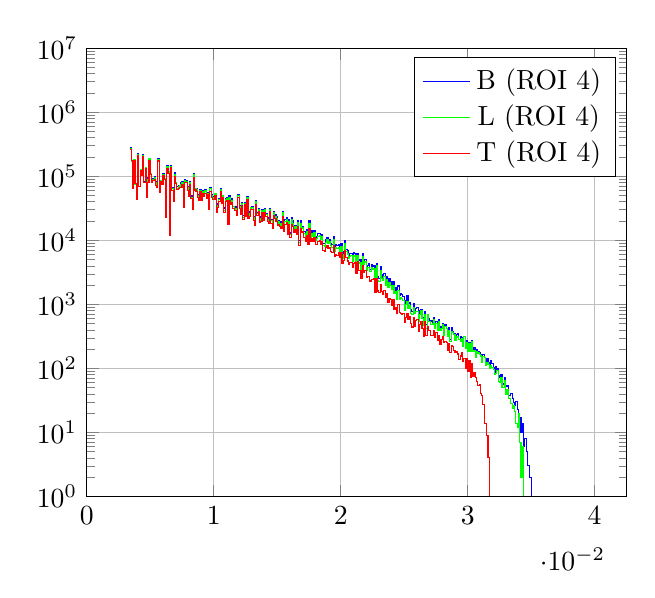
\begin{tikzpicture}

% Axis at [0.13 0.11 0.78 0.81]
\begin{semilogyaxis}[
xmajorgrids,
ymajorgrids,
xmin=0, xmax=0.0425,
ymin=1, ymax=1e+007,
%title={ROI 4},
legend entries={%
	B (ROI 4),%
	L (ROI 4),%
	T (ROI 4)}
]

\addplot [
color=blue,
solid
]coordinates{
 (0.0034,0) (0.0034,281790) (0.0034,281790) (0.0035,281790) (0.0035,168687) (0.0035,168687) (0.0036,168687) (0.0036,64147) (0.0036,64147) (0.0037,64147) (0.0037,183472) (0.0037,183472) (0.0038,183472) (0.0038,74451) (0.0038,74451) (0.0039,74451) (0.0039,51365) (0.0039,51365) (0.004,51365) (0.004,224801) (0.004,224801) (0.0041,224801) (0.0041,70097) (0.0041,70097) (0.0042,70097) (0.0042,125212) (0.0042,125212) (0.0043,125212) (0.0043,109648) (0.0043,109648) (0.0044,109648) (0.0044,217207) (0.0044,217207) (0.0045,217207) (0.0045,81721) (0.0045,81721) (0.0046,81721) (0.0046,138624) (0.0046,138624) (0.0047,138624) (0.0047,46672) (0.0047,46672) (0.0048,46672) (0.0048,94805) (0.0048,94805) (0.0049,94805) (0.0049,187740) (0.0049,187740) (0.005,187740) (0.005,109370) (0.005,109370) (0.0051,109370) (0.0051,82301) (0.0051,82301) (0.0052,82301) (0.0052,92493) (0.0052,92493) (0.0053,92493) (0.0053,97228) (0.0053,97228) (0.0054,97228) (0.0054,83152) (0.0054,83152) (0.0055,83152) (0.0055,68662) (0.0055,68662) (0.0056,68662) (0.0056,188624) (0.0056,188624) (0.0057,188624) (0.0057,60984) (0.0057,60984) (0.0058,60984) (0.0058,85874) (0.0058,85874) (0.0059,85874) (0.0059,86027) (0.0059,86027) (0.006,86027) (0.006,109570) (0.006,109570) (0.0061,109570) (0.0061,93178) (0.0061,93178) (0.0062,93178) (0.0062,28103) (0.0062,28103) (0.0063,28103) (0.0063,147873) (0.0063,147873) (0.0064,147873) (0.0064,119602) (0.0064,119602) (0.0065,119602) (0.0065,13881) (0.0065,13881) (0.0066,13881) (0.0066,147520) (0.0066,147520) (0.0067,147520) (0.0067,66635) (0.0067,66635) (0.0068,66635) (0.0068,50370) (0.0068,50370) (0.0069,50370) (0.0069,113021) (0.0069,113021) (0.007,113021) (0.007,79064) (0.007,79064) (0.0071,79064) (0.0071,68305) (0.0071,68305) (0.0072,68305) (0.0072,70929) (0.0072,70929) (0.0073,70929) (0.0073,72124) (0.0073,72124) (0.0074,72124) (0.0074,78397) (0.0074,78397) (0.0075,78397) (0.0075,82065) (0.0075,82065) (0.0076,82065) (0.0076,34686) (0.0076,34686) (0.0077,34686) (0.0077,88966) (0.0077,88966) (0.0078,88966) (0.0078,86468) (0.0078,86468) (0.0079,86468) (0.0079,68796) (0.0079,68796) (0.008,68796) (0.008,53451) (0.008,53451) (0.0081,53451) (0.0081,83440) (0.0081,83440) (0.0082,83440) (0.0082,49125) (0.0082,49125) (0.0083,49125) (0.0083,32723) (0.0083,32723) (0.0084,32723) (0.0084,110465) (0.0084,110465) (0.0085,110465) (0.0085,64697) (0.0085,64697) (0.0086,64697) (0.0086,63310) (0.0086,63310) (0.0087,63310) (0.0087,52216) (0.0087,52216) (0.0088,52216) (0.0088,48434) (0.0088,48434) (0.0089,48434) (0.0089,63050) (0.0089,63050) (0.009,63050) (0.009,46325) (0.009,46325) (0.0091,46325) (0.0091,58974) (0.0091,58974) (0.0092,58974) (0.0092,51474) (0.0092,51474) (0.0093,51474) (0.0093,61839) (0.0093,61839) (0.0094,61839) (0.0094,49505) (0.0094,49505) (0.0095,49505) (0.0095,55442) (0.0095,55442) (0.0096,55442) (0.0096,33007) (0.0096,33007) (0.0097,33007) (0.0097,67081) (0.0097,67081) (0.0098,67081) (0.0098,52082) (0.0098,52082) (0.0099,52082) (0.0099,46933) (0.0099,46933) (0.01,46933) (0.01,47979) (0.01,47979) (0.0101,47979) (0.0101,54391) (0.0101,54391) (0.0102,54391) (0.0102,30963) (0.0102,30963) (0.0103,30963) (0.0103,37071) (0.0103,37071) (0.0104,37071) (0.0104,45197) (0.0104,45197) (0.0105,45197) (0.0105,64518) (0.0105,64518) (0.0106,64518) (0.0106,41823) (0.0106,41823) (0.0107,41823) (0.0107,50716) (0.0107,50716) (0.0108,50716) (0.0108,31938) (0.0108,31938) (0.0109,31938) (0.0109,45127) (0.0109,45127) (0.011,45127) (0.011,46570) (0.011,46570) (0.0111,46570) (0.0111,20126) (0.0111,20126) (0.0112,20126) (0.0112,49088) (0.0112,49088) (0.0113,49088) (0.0113,41188) (0.0113,41188) (0.0114,41188) (0.0114,44329) (0.0114,44329) (0.0115,44329) (0.0115,34083) (0.0115,34083) (0.0116,34083) (0.0116,32041) (0.0116,32041) (0.0117,32041) (0.0117,33471) (0.0117,33471) (0.0118,33471) (0.0118,27855) (0.0118,27855) (0.0119,27855) (0.0119,52516) (0.0119,52516) (0.012,52516) (0.012,34779) (0.012,34779) (0.0121,34779) (0.0121,27427) (0.0121,27427) (0.0122,27427) (0.0122,38907) (0.0122,38907) (0.0123,38907) (0.0123,24409) (0.0123,24409) (0.0124,24409) (0.0124,39216) (0.0124,39216) (0.0125,39216) (0.0125,27562) (0.0125,27562) (0.0126,27562) (0.0126,47965) (0.0126,47965) (0.0127,47965) (0.0127,24612) (0.0127,24612) (0.0128,24612) (0.0128,28161) (0.0128,28161) (0.0129,28161) (0.0129,32843) (0.0129,32843) (0.013,32843) (0.013,33974) (0.013,33974) (0.0131,33974) (0.0131,23639) (0.0131,23639) (0.0132,23639) (0.0132,19381) (0.0132,19381) (0.0133,19381) (0.0133,41832) (0.0133,41832) (0.0134,41832) (0.0134,27262) (0.0134,27262) (0.0135,27262) (0.0135,31270) (0.0135,31270) (0.0136,31270) (0.0136,21165) (0.0136,21165) (0.0137,21165) (0.0137,23576) (0.0137,23576) (0.0138,23576) (0.0138,30490) (0.0138,30490) (0.0139,30490) (0.0139,23321) (0.0139,23321) (0.014,23321) (0.014,31710) (0.014,31710) (0.0141,31710) (0.0141,26187) (0.0141,26187) (0.0142,26187) (0.0142,22554) (0.0142,22554) (0.0143,22554) (0.0143,20740) (0.0143,20740) (0.0144,20740) (0.0144,31666) (0.0144,31666) (0.0145,31666) (0.0145,21389) (0.0145,21389) (0.0146,21389) (0.0146,17944) (0.0146,17944) (0.0147,17944) (0.0147,28503) (0.0147,28503) (0.0148,28503) (0.0148,25147) (0.0148,25147) (0.0149,25147) (0.0149,23160) (0.0149,23160) (0.015,23160) (0.015,19073) (0.015,19073) (0.0151,19073) (0.0151,20413) (0.0151,20413) (0.0152,20413) (0.0152,19280) (0.0152,19280) (0.0153,19280) (0.0153,18483) (0.0153,18483) (0.0154,18483) (0.0154,28334) (0.0154,28334) (0.0155,28334) (0.0155,15680) (0.0155,15680) (0.0156,15680) (0.0156,21249) (0.0156,21249) (0.0157,21249) (0.0157,22746) (0.0157,22746) (0.0158,22746) (0.0158,14662) (0.0158,14662) (0.0159,14662) (0.0159,21386) (0.0159,21386) (0.016,21386) (0.016,13020) (0.016,13020) (0.0161,13020) (0.0161,22399) (0.0161,22399) (0.0162,22399) (0.0162,20017) (0.0162,20017) (0.0163,20017) (0.0163,16458) (0.0163,16458) (0.0164,16458) (0.0164,17252) (0.0164,17252) (0.0165,17252) (0.0165,15524) (0.0165,15524) (0.0166,15524) (0.0166,20194) (0.0166,20194) (0.0167,20194) (0.0167,9839) (0.0167,9839) (0.0168,9839) (0.0168,20232) (0.0168,20232) (0.0169,20232) (0.0169,16104) (0.0169,16104) (0.017,16104) (0.017,16666) (0.017,16666) (0.0171,16666) (0.0171,13762) (0.0171,13762) (0.0172,13762) (0.0172,12442) (0.0172,12442) (0.0173,12442) (0.0173,14897) (0.0173,14897) (0.0174,14897) (0.0174,10641) (0.0174,10641) (0.0175,10641) (0.0175,20155) (0.0175,20155) (0.0176,20155) (0.0176,11833) (0.0176,11833) (0.0177,11833) (0.0177,14078) (0.0177,14078) (0.0178,14078) (0.0178,12455) (0.0178,12455) (0.0179,12455) (0.0179,14163) (0.0179,14163) (0.018,14163) (0.018,10944) (0.018,10944) (0.0181,10944) (0.0181,11617) (0.0181,11617) (0.0182,11617) (0.0182,12567) (0.0182,12567) (0.0183,12567) (0.0183,12826) (0.0183,12826) (0.0184,12826) (0.0184,11283) (0.0184,11283) (0.0185,11283) (0.0185,12297) (0.0185,12297) (0.0186,12297) (0.0186,8971) (0.0186,8971) (0.0187,8971) (0.0187,8952) (0.0187,8952) (0.0188,8952) (0.0188,10246) (0.0188,10246) (0.0189,10246) (0.0189,11137) (0.0189,11137) (0.019,11137) (0.019,9710) (0.019,9710) (0.0191,9710) (0.0191,10331) (0.0191,10331) (0.0192,10331) (0.0192,8949) (0.0192,8949) (0.0193,8949) (0.0193,8504) (0.0193,8504) (0.0194,8504) (0.0194,11245) (0.0194,11245) (0.0195,11245) (0.0195,7406) (0.0195,7406) (0.0196,7406) (0.0196,8475) (0.0196,8475) (0.0197,8475) (0.0197,8179) (0.0197,8179) (0.0198,8179) (0.0198,8496) (0.0198,8496) (0.0199,8496) (0.0199,7178) (0.0199,7178) (0.02,7178) (0.02,8824) (0.02,8824) (0.0201,8824) (0.0201,5735) (0.0201,5735) (0.0202,5735) (0.0202,6746) (0.0202,6746) (0.0203,6746) (0.0203,9878) (0.0203,9878) (0.0204,9878) (0.0204,7175) (0.0204,7175) (0.0205,7175) (0.0205,6824) (0.0205,6824) (0.0206,6824) (0.0206,5743) (0.0206,5743) (0.0207,5743) (0.0207,6270) (0.0207,6270) (0.0208,6270) (0.0208,6239) (0.0208,6239) (0.0209,6239) (0.0209,5107) (0.0209,5107) (0.021,5107) (0.021,6425) (0.021,6425) (0.0211,6425) (0.0211,6234) (0.0211,6234) (0.0212,6234) (0.0212,4529) (0.0212,4529) (0.0213,4529) (0.0213,6309) (0.0213,6309) (0.0214,6309) (0.0214,4819) (0.0214,4819) (0.0215,4819) (0.0215,4919) (0.0215,4919) (0.0216,4919) (0.0216,3530) (0.0216,3530) (0.0217,3530) (0.0217,6248) (0.0217,6248) (0.0218,6248) (0.0218,4633) (0.0218,4633) (0.0219,4633) (0.0219,5022) (0.0219,5022) (0.022,5022) (0.022,3834) (0.022,3834) (0.0221,3834) (0.0221,4067) (0.0221,4067) (0.0222,4067) (0.0222,4313) (0.0222,4313) (0.0223,4313) (0.0223,3554) (0.0223,3554) (0.0224,3554) (0.0224,4208) (0.0224,4208) (0.0225,4208) (0.0225,3888) (0.0225,3888) (0.0226,3888) (0.0226,3964) (0.0226,3964) (0.0227,3964) (0.0227,2656) (0.0227,2656) (0.0228,2656) (0.0228,4399) (0.0228,4399) (0.0229,4399) (0.0229,2691) (0.0229,2691) (0.023,2691) (0.023,2559) (0.023,2559) (0.0231,2559) (0.0231,3889) (0.0231,3889) (0.0232,3889) (0.0232,2942) (0.0232,2942) (0.0233,2942) (0.0233,2648) (0.0233,2648) (0.0234,2648) (0.0234,3073) (0.0234,3073) (0.0235,3073) (0.0235,2284) (0.0235,2284) (0.0236,2284) (0.0236,2758) (0.0236,2758) (0.0237,2758) (0.0237,2133) (0.0237,2133) (0.0238,2133) (0.0238,2532) (0.0238,2532) (0.0239,2532) (0.0239,2306) (0.0239,2306) (0.024,2306) (0.024,1965) (0.024,1965) (0.0241,1965) (0.0241,2298) (0.0241,2298) (0.0242,2298) (0.0242,1673) (0.0242,1673) (0.0243,1673) (0.0243,1843) (0.0243,1843) (0.0244,1843) (0.0244,1467) (0.0244,1467) (0.0245,1467) (0.0245,1935) (0.0245,1935) (0.0246,1935) (0.0246,1377) (0.0246,1377) (0.0247,1377) (0.0247,1459) (0.0247,1459) (0.0248,1459) (0.0248,1423) (0.0248,1423) (0.0249,1423) (0.0249,1346) (0.0249,1346) (0.025,1346) (0.025,947) (0.025,947) (0.0251,947) (0.0251,1162) (0.0251,1162) (0.0252,1162) (0.0252,1351) (0.0252,1351) (0.0253,1351) (0.0253,1019) (0.0253,1019) (0.0254,1019) (0.0254,1058) (0.0254,1058) (0.0255,1058) (0.0255,832) (0.0255,832) (0.0256,832) (0.0256,783) (0.0256,783) (0.0257,783) (0.0257,1018) (0.0257,1018) (0.0258,1018) (0.0258,801) (0.0258,801) (0.0259,801) (0.0259,867) (0.0259,867) (0.026,867) (0.026,887) (0.026,887) (0.0261,887) (0.0261,571) (0.0261,571) (0.0262,571) (0.0262,803) (0.0262,803) (0.0263,803) (0.0263,825) (0.0263,825) (0.0264,825) (0.0264,631) (0.0264,631) (0.0265,631) (0.0265,527) (0.0265,527) (0.0266,527) (0.0266,759) (0.0266,759) (0.0267,759) (0.0267,488) (0.0267,488) (0.0268,488) (0.0268,686) (0.0268,686) (0.0269,686) (0.0269,590) (0.0269,590) (0.027,590) (0.027,568) (0.027,568) (0.0271,568) (0.0271,549) (0.0271,549) (0.0272,549) (0.0272,506) (0.0272,506) (0.0273,506) (0.0273,619) (0.0273,619) (0.0274,619) (0.0274,432) (0.0274,432) (0.0275,432) (0.0275,543) (0.0275,543) (0.0276,543) (0.0276,411) (0.0276,411) (0.0277,411) (0.0277,575) (0.0277,575) (0.0278,575) (0.0278,413) (0.0278,413) (0.0279,413) (0.0279,451) (0.0279,451) (0.028,451) (0.028,508) (0.028,508) (0.0281,508) (0.0281,370) (0.0281,370) (0.0282,370) (0.0282,475) (0.0282,475) (0.0283,475) (0.0283,423) (0.0283,423) (0.0284,423) (0.0284,338) (0.0284,338) (0.0285,338) (0.0285,434) (0.0285,434) (0.0286,434) (0.0286,283) (0.0286,283) (0.0287,283) (0.0287,433) (0.0287,433) (0.0288,433) (0.0288,375) (0.0288,375) (0.0289,375) (0.0289,347) (0.0289,347) (0.029,347) (0.029,288) (0.029,288) (0.0291,288) (0.0291,337) (0.0291,337) (0.0292,337) (0.0292,344) (0.0292,344) (0.0293,344) (0.0293,280) (0.0293,280) (0.0294,280) (0.0294,317) (0.0294,317) (0.0295,317) (0.0295,298) (0.0295,298) (0.0296,298) (0.0296,244) (0.0296,244) (0.0297,244) (0.0297,313) (0.0297,313) (0.0298,313) (0.0298,227) (0.0298,227) (0.0299,227) (0.0299,271) (0.0299,271) (0.03,271) (0.03,222) (0.03,222) (0.0301,222) (0.0301,253) (0.0301,253) (0.0302,253) (0.0302,208) (0.0302,208) (0.0303,208) (0.0303,274) (0.0303,274) (0.0304,274) (0.0304,186) (0.0304,186) (0.0305,186) (0.0305,212) (0.0305,212) (0.0306,212) (0.0306,174) (0.0306,174) (0.0307,174) (0.0307,197) (0.0307,197) (0.0308,197) (0.0308,180) (0.0308,180) (0.0309,180) (0.0309,175) (0.0309,175) (0.031,175) (0.031,164) (0.031,164) (0.0311,164) (0.0311,161) (0.0311,161) (0.0312,161) (0.0312,164) (0.0312,164) (0.0313,164) (0.0313,147) (0.0313,147) (0.0314,147) (0.0314,117) (0.0314,117) (0.0315,117) (0.0315,142) (0.0315,142) (0.0316,142) (0.0316,123) (0.0316,123) (0.0317,123) (0.0317,110) (0.0317,110) (0.0318,110) (0.0318,131) (0.0318,131) (0.0319,131) (0.0319,118) (0.0319,118) (0.032,118) (0.032,103) (0.032,103) (0.0321,103) (0.0321,82) (0.0321,82) (0.0322,82) (0.0322,106) (0.0322,106) (0.0323,106) (0.0323,98) (0.0323,98) (0.0324,98) (0.0324,76) (0.0324,76) (0.0325,76) (0.0325,72) (0.0325,72) (0.0326,72) (0.0326,79) (0.0326,79) (0.0327,79) (0.0327,57) (0.0327,57) (0.0328,57) (0.0328,56) (0.0328,56) (0.0329,56) (0.0329,72) (0.0329,72) (0.033,72) (0.033,52) (0.033,52) (0.0331,52) (0.0331,54) (0.0331,54) (0.0332,54) (0.0332,38) (0.0332,38) (0.0333,38) (0.0333,38) (0.0333,38) (0.0334,38) (0.0334,40) (0.0334,40) (0.0335,40) (0.0335,34) (0.0335,34) (0.0336,34) (0.0336,29) (0.0336,29) (0.0337,29) (0.0337,26) (0.0337,26) (0.0338,26) (0.0338,30) (0.0338,30) (0.0339,30) (0.0339,23) (0.0339,23) (0.034,23) (0.034,16) (0.034,16) (0.0341,16) (0.0341,17) (0.0341,17) (0.0342,17) (0.0342,10) (0.0342,10) (0.0343,10) (0.0343,14) (0.0343,14) (0.0344,14) (0.0344,6) (0.0344,6) (0.0345,6) (0.0345,8) (0.0345,8) (0.0346,8) (0.0346,5) (0.0346,5) (0.0347,5) (0.0347,3) (0.0347,3) (0.0348,3) (0.0348,3) (0.0348,3) (0.0349,3) (0.0349,2) (0.0349,2) (0.035,2) (0.035,1)
};

\addplot [
color=green,
solid
]coordinates{
 (0.0034,0) (0.0034,271598) (0.0034,271598) (0.0035,271598) (0.0035,172321) (0.0035,172321) (0.0036,172321) (0.0036,64685) (0.0036,64685) (0.0037,64685) (0.0037,179388) (0.0037,179388) (0.0038,179388) (0.0038,75745) (0.0038,75745) (0.0039,75745) (0.0039,48485) (0.0039,48485) (0.004,48485) (0.004,217792) (0.004,217792) (0.0041,217792) (0.0041,69854) (0.0041,69854) (0.0042,69854) (0.0042,125340) (0.0042,125340) (0.0043,125340) (0.0043,106837) (0.0043,106837) (0.0044,106837) (0.0044,211120) (0.0044,211120) (0.0045,211120) (0.0045,81090) (0.0045,81090) (0.0046,81090) (0.0046,134794) (0.0046,134794) (0.0047,134794) (0.0047,46636) (0.0047,46636) (0.0048,46636) (0.0048,87452) (0.0048,87452) (0.0049,87452) (0.0049,185602) (0.0049,185602) (0.005,185602) (0.005,108285) (0.005,108285) (0.0051,108285) (0.0051,80595) (0.0051,80595) (0.0052,80595) (0.0052,89130) (0.0052,89130) (0.0053,89130) (0.0053,93871) (0.0053,93871) (0.0054,93871) (0.0054,78797) (0.0054,78797) (0.0055,78797) (0.0055,68352) (0.0055,68352) (0.0056,68352) (0.0056,183152) (0.0056,183152) (0.0057,183152) (0.0057,59111) (0.0057,59111) (0.0058,59111) (0.0058,84509) (0.0058,84509) (0.0059,84509) (0.0059,81333) (0.0059,81333) (0.006,81333) (0.006,106593) (0.006,106593) (0.0061,106593) (0.0061,91206) (0.0061,91206) (0.0062,91206) (0.0062,26292) (0.0062,26292) (0.0063,26292) (0.0063,141663) (0.0063,141663) (0.0064,141663) (0.0064,117076) (0.0064,117076) (0.0065,117076) (0.0065,13013) (0.0065,13013) (0.0066,13013) (0.0066,143979) (0.0066,143979) (0.0067,143979) (0.0067,63455) (0.0067,63455) (0.0068,63455) (0.0068,46376) (0.0068,46376) (0.0069,46376) (0.0069,107528) (0.0069,107528) (0.007,107528) (0.007,78585) (0.007,78585) (0.0071,78585) (0.0071,65388) (0.0071,65388) (0.0072,65388) (0.0072,67906) (0.0072,67906) (0.0073,67906) (0.0073,70405) (0.0073,70405) (0.0074,70405) (0.0074,73895) (0.0074,73895) (0.0075,73895) (0.0075,79291) (0.0075,79291) (0.0076,79291) (0.0076,33761) (0.0076,33761) (0.0077,33761) (0.0077,84818) (0.0077,84818) (0.0078,84818) (0.0078,83367) (0.0078,83367) (0.0079,83367) (0.0079,65594) (0.0079,65594) (0.008,65594) (0.008,51344) (0.008,51344) (0.0081,51344) (0.0081,80645) (0.0081,80645) (0.0082,80645) (0.0082,47268) (0.0082,47268) (0.0083,47268) (0.0083,31366) (0.0083,31366) (0.0084,31366) (0.0084,104659) (0.0084,104659) (0.0085,104659) (0.0085,63417) (0.0085,63417) (0.0086,63417) (0.0086,61457) (0.0086,61457) (0.0087,61457) (0.0087,50171) (0.0087,50171) (0.0088,50171) (0.0088,45566) (0.0088,45566) (0.0089,45566) (0.0089,60555) (0.0089,60555) (0.009,60555) (0.009,44454) (0.009,44454) (0.0091,44454) (0.0091,57312) (0.0091,57312) (0.0092,57312) (0.0092,50260) (0.0092,50260) (0.0093,50260) (0.0093,58793) (0.0093,58793) (0.0094,58793) (0.0094,47298) (0.0094,47298) (0.0095,47298) (0.0095,54373) (0.0095,54373) (0.0096,54373) (0.0096,31927) (0.0096,31927) (0.0097,31927) (0.0097,63527) (0.0097,63527) (0.0098,63527) (0.0098,50304) (0.0098,50304) (0.0099,50304) (0.0099,45391) (0.0099,45391) (0.01,45391) (0.01,46241) (0.01,46241) (0.0101,46241) (0.0101,52768) (0.0101,52768) (0.0102,52768) (0.0102,29422) (0.0102,29422) (0.0103,29422) (0.0103,35054) (0.0103,35054) (0.0104,35054) (0.0104,43319) (0.0104,43319) (0.0105,43319) (0.0105,61777) (0.0105,61777) (0.0106,61777) (0.0106,40538) (0.0106,40538) (0.0107,40538) (0.0107,49448) (0.0107,49448) (0.0108,49448) (0.0108,29661) (0.0108,29661) (0.0109,29661) (0.0109,43735) (0.0109,43735) (0.011,43735) (0.011,44987) (0.011,44987) (0.0111,44987) (0.0111,19068) (0.0111,19068) (0.0112,19068) (0.0112,46720) (0.0112,46720) (0.0113,46720) (0.0113,39601) (0.0113,39601) (0.0114,39601) (0.0114,42456) (0.0114,42456) (0.0115,42456) (0.0115,33219) (0.0115,33219) (0.0116,33219) (0.0116,30804) (0.0116,30804) (0.0117,30804) (0.0117,31753) (0.0117,31753) (0.0118,31753) (0.0118,26259) (0.0118,26259) (0.0119,26259) (0.0119,50388) (0.0119,50388) (0.012,50388) (0.012,33765) (0.012,33765) (0.0121,33765) (0.0121,26360) (0.0121,26360) (0.0122,26360) (0.0122,37251) (0.0122,37251) (0.0123,37251) (0.0123,22864) (0.0123,22864) (0.0124,22864) (0.0124,38087) (0.0124,38087) (0.0125,38087) (0.0125,25879) (0.0125,25879) (0.0126,25879) (0.0126,46307) (0.0126,46307) (0.0127,46307) (0.0127,23698) (0.0127,23698) (0.0128,23698) (0.0128,26526) (0.0128,26526) (0.0129,26526) (0.0129,31901) (0.0129,31901) (0.013,31901) (0.013,32519) (0.013,32519) (0.0131,32519) (0.0131,22345) (0.0131,22345) (0.0132,22345) (0.0132,18597) (0.0132,18597) (0.0133,18597) (0.0133,39876) (0.0133,39876) (0.0134,39876) (0.0134,25938) (0.0134,25938) (0.0135,25938) (0.0135,30158) (0.0135,30158) (0.0136,30158) (0.0136,20354) (0.0136,20354) (0.0137,20354) (0.0137,22184) (0.0137,22184) (0.0138,22184) (0.0138,28964) (0.0138,28964) (0.0139,28964) (0.0139,22057) (0.0139,22057) (0.014,22057) (0.014,30233) (0.014,30233) (0.0141,30233) (0.0141,25127) (0.0141,25127) (0.0142,25127) (0.0142,21408) (0.0142,21408) (0.0143,21408) (0.0143,19627) (0.0143,19627) (0.0144,19627) (0.0144,30202) (0.0144,30202) (0.0145,30202) (0.0145,20136) (0.0145,20136) (0.0146,20136) (0.0146,16800) (0.0146,16800) (0.0147,16800) (0.0147,26933) (0.0147,26933) (0.0148,26933) (0.0148,23822) (0.0148,23822) (0.0149,23822) (0.0149,21923) (0.0149,21923) (0.015,21923) (0.015,18236) (0.015,18236) (0.0151,18236) (0.0151,19299) (0.0151,19299) (0.0152,19299) (0.0152,18011) (0.0152,18011) (0.0153,18011) (0.0153,17154) (0.0153,17154) (0.0154,17154) (0.0154,26735) (0.0154,26735) (0.0155,26735) (0.0155,14903) (0.0155,14903) (0.0156,14903) (0.0156,19867) (0.0156,19867) (0.0157,19867) (0.0157,21405) (0.0157,21405) (0.0158,21405) (0.0158,13716) (0.0158,13716) (0.0159,13716) (0.0159,19819) (0.0159,19819) (0.016,19819) (0.016,12277) (0.016,12277) (0.0161,12277) (0.0161,20789) (0.0161,20789) (0.0162,20789) (0.0162,18563) (0.0162,18563) (0.0163,18563) (0.0163,15371) (0.0163,15371) (0.0164,15371) (0.0164,16192) (0.0164,16192) (0.0165,16192) (0.0165,14460) (0.0165,14460) (0.0166,14460) (0.0166,18838) (0.0166,18838) (0.0167,18838) (0.0167,9349) (0.0167,9349) (0.0168,9349) (0.0168,18416) (0.0168,18416) (0.0169,18416) (0.0169,15104) (0.0169,15104) (0.017,15104) (0.017,15620) (0.017,15620) (0.0171,15620) (0.0171,12651) (0.0171,12651) (0.0172,12651) (0.0172,11357) (0.0172,11357) (0.0173,11357) (0.0173,13827) (0.0173,13827) (0.0174,13827) (0.0174,9864) (0.0174,9864) (0.0175,9864) (0.0175,18316) (0.0175,18316) (0.0176,18316) (0.0176,11046) (0.0176,11046) (0.0177,11046) (0.0177,12974) (0.0177,12974) (0.0178,12974) (0.0178,11409) (0.0178,11409) (0.0179,11409) (0.0179,13029) (0.0179,13029) (0.018,13029) (0.018,10006) (0.018,10006) (0.0181,10006) (0.0181,10551) (0.0181,10551) (0.0182,10551) (0.0182,11614) (0.0182,11614) (0.0183,11614) (0.0183,11684) (0.0183,11684) (0.0184,11684) (0.0184,10377) (0.0184,10377) (0.0185,10377) (0.0185,11342) (0.0185,11342) (0.0186,11342) (0.0186,8325) (0.0186,8325) (0.0187,8325) (0.0187,8153) (0.0187,8153) (0.0188,8153) (0.0188,9281) (0.0188,9281) (0.0189,9281) (0.0189,10287) (0.0189,10287) (0.019,10287) (0.019,9052) (0.019,9052) (0.0191,9052) (0.0191,9436) (0.0191,9436) (0.0192,9436) (0.0192,8165) (0.0192,8165) (0.0193,8165) (0.0193,7714) (0.0193,7714) (0.0194,7714) (0.0194,10363) (0.0194,10363) (0.0195,10363) (0.0195,6733) (0.0195,6733) (0.0196,6733) (0.0196,7744) (0.0196,7744) (0.0197,7744) (0.0197,7366) (0.0197,7366) (0.0198,7366) (0.0198,7824) (0.0198,7824) (0.0199,7824) (0.0199,6639) (0.0199,6639) (0.02,6639) (0.02,7922) (0.02,7922) (0.0201,7922) (0.0201,5288) (0.0201,5288) (0.0202,5288) (0.0202,6066) (0.0202,6066) (0.0203,6066) (0.0203,8871) (0.0203,8871) (0.0204,8871) (0.0204,6669) (0.0204,6669) (0.0205,6669) (0.0205,6103) (0.0205,6103) (0.0206,6103) (0.0206,5292) (0.0206,5292) (0.0207,5292) (0.0207,5580) (0.0207,5580) (0.0208,5580) (0.0208,5713) (0.0208,5713) (0.0209,5713) (0.0209,4593) (0.0209,4593) (0.021,4593) (0.021,5820) (0.021,5820) (0.0211,5820) (0.0211,5687) (0.0211,5687) (0.0212,5687) (0.0212,4029) (0.0212,4029) (0.0213,4029) (0.0213,5764) (0.0213,5764) (0.0214,5764) (0.0214,4410) (0.0214,4410) (0.0215,4410) (0.0215,4435) (0.0215,4435) (0.0216,4435) (0.0216,3203) (0.0216,3203) (0.0217,3203) (0.0217,5529) (0.0217,5529) (0.0218,5529) (0.0218,4174) (0.0218,4174) (0.0219,4174) (0.0219,4591) (0.0219,4591) (0.022,4591) (0.022,3386) (0.022,3386) (0.0221,3386) (0.0221,3728) (0.0221,3728) (0.0222,3728) (0.0222,3796) (0.0222,3796) (0.0223,3796) (0.0223,3242) (0.0223,3242) (0.0224,3242) (0.0224,3713) (0.0224,3713) (0.0225,3713) (0.0225,3507) (0.0225,3507) (0.0226,3507) (0.0226,3565) (0.0226,3565) (0.0227,3565) (0.0227,2296) (0.0227,2296) (0.0228,2296) (0.0228,3967) (0.0228,3967) (0.0229,3967) (0.0229,2394) (0.0229,2394) (0.023,2394) (0.023,2269) (0.023,2269) (0.0231,2269) (0.0231,3410) (0.0231,3410) (0.0232,3410) (0.0232,2520) (0.0232,2520) (0.0233,2520) (0.0233,2320) (0.0233,2320) (0.0234,2320) (0.0234,2752) (0.0234,2752) (0.0235,2752) (0.0235,1999) (0.0235,1999) (0.0236,1999) (0.0236,2428) (0.0236,2428) (0.0237,2428) (0.0237,1857) (0.0237,1857) (0.0238,1857) (0.0238,2150) (0.0238,2150) (0.0239,2150) (0.0239,1998) (0.0239,1998) (0.024,1998) (0.024,1685) (0.024,1685) (0.0241,1685) (0.0241,1984) (0.0241,1984) (0.0242,1984) (0.0242,1465) (0.0242,1465) (0.0243,1465) (0.0243,1588) (0.0243,1588) (0.0244,1588) (0.0244,1210) (0.0244,1210) (0.0245,1210) (0.0245,1650) (0.0245,1650) (0.0246,1650) (0.0246,1174) (0.0246,1174) (0.0247,1174) (0.0247,1257) (0.0247,1257) (0.0248,1257) (0.0248,1216) (0.0248,1216) (0.0249,1216) (0.0249,1146) (0.0249,1146) (0.025,1146) (0.025,803) (0.025,803) (0.0251,803) (0.0251,989) (0.0251,989) (0.0252,989) (0.0252,1110) (0.0252,1110) (0.0253,1110) (0.0253,849) (0.0253,849) (0.0254,849) (0.0254,973) (0.0254,973) (0.0255,973) (0.0255,713) (0.0255,713) (0.0256,713) (0.0256,686) (0.0256,686) (0.0257,686) (0.0257,881) (0.0257,881) (0.0258,881) (0.0258,714) (0.0258,714) (0.0259,714) (0.0259,766) (0.0259,766) (0.026,766) (0.026,769) (0.026,769) (0.0261,769) (0.0261,541) (0.0261,541) (0.0262,541) (0.0262,699) (0.0262,699) (0.0263,699) (0.0263,796) (0.0263,796) (0.0264,796) (0.0264,603) (0.0264,603) (0.0265,603) (0.0265,464) (0.0265,464) (0.0266,464) (0.0266,691) (0.0266,691) (0.0267,691) (0.0267,425) (0.0267,425) (0.0268,425) (0.0268,689) (0.0268,689) (0.0269,689) (0.0269,546) (0.0269,546) (0.027,546) (0.027,548) (0.027,548) (0.0271,548) (0.0271,485) (0.0271,485) (0.0272,485) (0.0272,494) (0.0272,494) (0.0273,494) (0.0273,576) (0.0273,576) (0.0274,576) (0.0274,426) (0.0274,426) (0.0275,426) (0.0275,507) (0.0275,507) (0.0276,507) (0.0276,397) (0.0276,397) (0.0277,397) (0.0277,537) (0.0277,537) (0.0278,537) (0.0278,396) (0.0278,396) (0.0279,396) (0.0279,420) (0.0279,420) (0.028,420) (0.028,478) (0.028,478) (0.0281,478) (0.0281,324) (0.0281,324) (0.0282,324) (0.0282,450) (0.0282,450) (0.0283,450) (0.0283,423) (0.0283,423) (0.0284,423) (0.0284,317) (0.0284,317) (0.0285,317) (0.0285,396) (0.0285,396) (0.0286,396) (0.0286,264) (0.0286,264) (0.0287,264) (0.0287,381) (0.0287,381) (0.0288,381) (0.0288,364) (0.0288,364) (0.0289,364) (0.0289,341) (0.0289,341) (0.029,341) (0.029,271) (0.029,271) (0.0291,271) (0.0291,311) (0.0291,311) (0.0292,311) (0.0292,309) (0.0292,309) (0.0293,309) (0.0293,279) (0.0293,279) (0.0294,279) (0.0294,264) (0.0294,264) (0.0295,264) (0.0295,292) (0.0295,292) (0.0296,292) (0.0296,217) (0.0296,217) (0.0297,217) (0.0297,315) (0.0297,315) (0.0298,315) (0.0298,208) (0.0298,208) (0.0299,208) (0.0299,257) (0.0299,257) (0.03,257) (0.03,184) (0.03,184) (0.0301,184) (0.0301,244) (0.0301,244) (0.0302,244) (0.0302,185) (0.0302,185) (0.0303,185) (0.0303,260) (0.0303,260) (0.0304,260) (0.0304,183) (0.0304,183) (0.0305,183) (0.0305,191) (0.0305,191) (0.0306,191) (0.0306,147) (0.0306,147) (0.0307,147) (0.0307,181) (0.0307,181) (0.0308,181) (0.0308,174) (0.0308,174) (0.0309,174) (0.0309,166) (0.0309,166) (0.031,166) (0.031,156) (0.031,156) (0.0311,156) (0.0311,122) (0.0311,122) (0.0312,122) (0.0312,152) (0.0312,152) (0.0313,152) (0.0313,146) (0.0313,146) (0.0314,146) (0.0314,110) (0.0314,110) (0.0315,110) (0.0315,124) (0.0315,124) (0.0316,124) (0.0316,115) (0.0316,115) (0.0317,115) (0.0317,99) (0.0317,99) (0.0318,99) (0.0318,111) (0.0318,111) (0.0319,111) (0.0319,104) (0.0319,104) (0.032,104) (0.032,95) (0.032,95) (0.0321,95) (0.0321,80) (0.0321,80) (0.0322,80) (0.0322,83) (0.0322,83) (0.0323,83) (0.0323,92) (0.0323,92) (0.0324,92) (0.0324,63) (0.0324,63) (0.0325,63) (0.0325,61) (0.0325,61) (0.0326,61) (0.0326,72) (0.0326,72) (0.0327,72) (0.0327,51) (0.0327,51) (0.0328,51) (0.0328,50) (0.0328,50) (0.0329,50) (0.0329,64) (0.0329,64) (0.033,64) (0.033,39) (0.033,39) (0.0331,39) (0.0331,46) (0.0331,46) (0.0332,46) (0.0332,34) (0.0332,34) (0.0333,34) (0.0333,34) (0.0333,34) (0.0334,34) (0.0334,28) (0.0334,28) (0.0335,28) (0.0335,24) (0.0335,24) (0.0336,24) (0.0336,26) (0.0336,26) (0.0337,26) (0.0337,21) (0.0337,21) (0.0338,21) (0.0338,14) (0.0338,14) (0.0339,14) (0.0339,12) (0.0339,12) (0.034,12) (0.034,20) (0.034,20) (0.0341,20) (0.0341,7) (0.0341,7) (0.0342,7) (0.0342,2) (0.0342,2) (0.0343,2) (0.0343,6) (0.0343,6) (0.0344,6) (0.0344,1)
};

\addplot [
color=red,
solid
]coordinates{
 (0.0034,0) (0.0034,257512) (0.0034,257512) (0.0035,257512) (0.0035,175936) (0.0035,175936) (0.0036,175936) (0.0036,64707) (0.0036,64707) (0.0037,64707) (0.0037,174999) (0.0037,174999) (0.0038,174999) (0.0038,77453) (0.0038,77453) (0.0039,77453) (0.0039,43250) (0.0039,43250) (0.004,43250) (0.004,208640) (0.004,208640) (0.0041,208640) (0.0041,70071) (0.0041,70071) (0.0042,70071) (0.0042,123520) (0.0042,123520) (0.0043,123520) (0.0043,104650) (0.0043,104650) (0.0044,104650) (0.0044,200969) (0.0044,200969) (0.0045,200969) (0.0045,80123) (0.0045,80123) (0.0046,80123) (0.0046,129656) (0.0046,129656) (0.0047,129656) (0.0047,46922) (0.0047,46922) (0.0048,46922) (0.0048,80160) (0.0048,80160) (0.0049,80160) (0.0049,178102) (0.0049,178102) (0.005,178102) (0.005,105383) (0.005,105383) (0.0051,105383) (0.0051,78942) (0.0051,78942) (0.0052,78942) (0.0052,84976) (0.0052,84976) (0.0053,84976) (0.0053,88634) (0.0053,88634) (0.0054,88634) (0.0054,72584) (0.0054,72584) (0.0055,72584) (0.0055,67808) (0.0055,67808) (0.0056,67808) (0.0056,172941) (0.0056,172941) (0.0057,172941) (0.0057,56236) (0.0057,56236) (0.0058,56236) (0.0058,82668) (0.0058,82668) (0.0059,82668) (0.0059,73316) (0.0059,73316) (0.006,73316) (0.006,102809) (0.006,102809) (0.0061,102809) (0.0061,88049) (0.0061,88049) (0.0062,88049) (0.0062,23100) (0.0062,23100) (0.0063,23100) (0.0063,133691) (0.0063,133691) (0.0064,133691) (0.0064,110880) (0.0064,110880) (0.0065,110880) (0.0065,11699) (0.0065,11699) (0.0066,11699) (0.0066,138069) (0.0066,138069) (0.0067,138069) (0.0067,59712) (0.0067,59712) (0.0068,59712) (0.0068,41068) (0.0068,41068) (0.0069,41068) (0.0069,99785) (0.0069,99785) (0.007,99785) (0.007,76300) (0.007,76300) (0.0071,76300) (0.0071,61808) (0.0071,61808) (0.0072,61808) (0.0072,63466) (0.0072,63466) (0.0073,63466) (0.0073,67204) (0.0073,67204) (0.0074,67204) (0.0074,67560) (0.0074,67560) (0.0075,67560) (0.0075,74727) (0.0075,74727) (0.0076,74727) (0.0076,32382) (0.0076,32382) (0.0077,32382) (0.0077,78728) (0.0077,78728) (0.0078,78728) (0.0078,78635) (0.0078,78635) (0.0079,78635) (0.0079,60280) (0.0079,60280) (0.008,60280) (0.008,48825) (0.008,48825) (0.0081,48825) (0.0081,75304) (0.0081,75304) (0.0082,75304) (0.0082,44920) (0.0082,44920) (0.0083,44920) (0.0083,29780) (0.0083,29780) (0.0084,29780) (0.0084,95358) (0.0084,95358) (0.0085,95358) (0.0085,60886) (0.0085,60886) (0.0086,60886) (0.0086,57853) (0.0086,57853) (0.0087,57853) (0.0087,47172) (0.0087,47172) (0.0088,47172) (0.0088,41409) (0.0088,41409) (0.0089,41409) (0.0089,56836) (0.0089,56836) (0.009,56836) (0.009,41330) (0.009,41330) (0.0091,41330) (0.0091,53077) (0.0091,53077) (0.0092,53077) (0.0092,48203) (0.0092,48203) (0.0093,48203) (0.0093,53776) (0.0093,53776) (0.0094,53776) (0.0094,44254) (0.0094,44254) (0.0095,44254) (0.0095,51518) (0.0095,51518) (0.0096,51518) (0.0096,30101) (0.0096,30101) (0.0097,30101) (0.0097,58681) (0.0097,58681) (0.0098,58681) (0.0098,46318) (0.0098,46318) (0.0099,46318) (0.0099,42753) (0.0099,42753) (0.01,42753) (0.01,43221) (0.01,43221) (0.0101,43221) (0.0101,49684) (0.0101,49684) (0.0102,49684) (0.0102,27346) (0.0102,27346) (0.0103,27346) (0.0103,32313) (0.0103,32313) (0.0104,32313) (0.0104,40301) (0.0104,40301) (0.0105,40301) (0.0105,57108) (0.0105,57108) (0.0106,57108) (0.0106,38153) (0.0106,38153) (0.0107,38153) (0.0107,46906) (0.0107,46906) (0.0108,46906) (0.0108,26860) (0.0108,26860) (0.0109,26860) (0.0109,40822) (0.0109,40822) (0.011,40822) (0.011,42438) (0.011,42438) (0.0111,42438) (0.0111,17934) (0.0111,17934) (0.0112,17934) (0.0112,42438) (0.0112,42438) (0.0113,42438) (0.0113,36831) (0.0113,36831) (0.0114,36831) (0.0114,39502) (0.0114,39502) (0.0115,39502) (0.0115,31420) (0.0115,31420) (0.0116,31420) (0.0116,28790) (0.0116,28790) (0.0117,28790) (0.0117,29421) (0.0117,29421) (0.0118,29421) (0.0118,24191) (0.0118,24191) (0.0119,24191) (0.0119,46052) (0.0119,46052) (0.012,46052) (0.012,31833) (0.012,31833) (0.0121,31833) (0.0121,24898) (0.0121,24898) (0.0122,24898) (0.0122,34593) (0.0122,34593) (0.0123,34593) (0.0123,20824) (0.0123,20824) (0.0124,20824) (0.0124,35883) (0.0124,35883) (0.0125,35883) (0.0125,23606) (0.0125,23606) (0.0126,23606) (0.0126,43044) (0.0126,43044) (0.0127,43044) (0.0127,22232) (0.0127,22232) (0.0128,22232) (0.0128,23634) (0.0128,23634) (0.0129,23634) (0.0129,30347) (0.0129,30347) (0.013,30347) (0.013,30300) (0.013,30300) (0.0131,30300) (0.0131,20632) (0.0131,20632) (0.0132,20632) (0.0132,17302) (0.0132,17302) (0.0133,17302) (0.0133,36249) (0.0133,36249) (0.0134,36249) (0.0134,24026) (0.0134,24026) (0.0135,24026) (0.0135,28236) (0.0135,28236) (0.0136,28236) (0.0136,19267) (0.0136,19267) (0.0137,19267) (0.0137,19825) (0.0137,19825) (0.0138,19825) (0.0138,26937) (0.0138,26937) (0.0139,26937) (0.0139,20150) (0.0139,20150) (0.014,20150) (0.014,27494) (0.014,27494) (0.0141,27494) (0.0141,23335) (0.0141,23335) (0.0142,23335) (0.0142,19784) (0.0142,19784) (0.0143,19784) (0.0143,18062) (0.0143,18062) (0.0144,18062) (0.0144,27792) (0.0144,27792) (0.0145,27792) (0.0145,18417) (0.0145,18417) (0.0146,18417) (0.0146,15169) (0.0146,15169) (0.0147,15169) (0.0147,24276) (0.0147,24276) (0.0148,24276) (0.0148,21703) (0.0148,21703) (0.0149,21703) (0.0149,19909) (0.0149,19909) (0.015,19909) (0.015,16758) (0.015,16758) (0.0151,16758) (0.0151,17548) (0.0151,17548) (0.0152,17548) (0.0152,16222) (0.0152,16222) (0.0153,16222) (0.0153,15129) (0.0153,15129) (0.0154,15129) (0.0154,23589) (0.0154,23589) (0.0155,23589) (0.0155,13705) (0.0155,13705) (0.0156,13705) (0.0156,17743) (0.0156,17743) (0.0157,17743) (0.0157,18862) (0.0157,18862) (0.0158,18862) (0.0158,12416) (0.0158,12416) (0.0159,12416) (0.0159,17599) (0.0159,17599) (0.016,17599) (0.016,11148) (0.016,11148) (0.0161,11148) (0.0161,17858) (0.0161,17858) (0.0162,17858) (0.0162,16229) (0.0162,16229) (0.0163,16229) (0.0163,13340) (0.0163,13340) (0.0164,13340) (0.0164,14713) (0.0164,14713) (0.0165,14713) (0.0165,12434) (0.0165,12434) (0.0166,12434) (0.0166,16406) (0.0166,16406) (0.0167,16406) (0.0167,8312) (0.0167,8312) (0.0168,8312) (0.0168,15420) (0.0168,15420) (0.0169,15420) (0.0169,13049) (0.0169,13049) (0.017,13049) (0.017,13467) (0.017,13467) (0.0171,13467) (0.0171,10894) (0.0171,10894) (0.0172,10894) (0.0172,9581) (0.0172,9581) (0.0173,9581) (0.0173,12018) (0.0173,12018) (0.0174,12018) (0.0174,8567) (0.0174,8567) (0.0175,8567) (0.0175,15169) (0.0175,15169) (0.0176,15169) (0.0176,9465) (0.0176,9465) (0.0177,9465) (0.0177,10818) (0.0177,10818) (0.0178,10818) (0.0178,9730) (0.0178,9730) (0.0179,9730) (0.0179,11160) (0.0179,11160) (0.018,11160) (0.018,8734) (0.018,8734) (0.0181,8734) (0.0181,8703) (0.0181,8703) (0.0182,8703) (0.0182,9478) (0.0182,9478) (0.0183,9478) (0.0183,9994) (0.0183,9994) (0.0184,9994) (0.0184,8676) (0.0184,8676) (0.0185,8676) (0.0185,9470) (0.0185,9470) (0.0186,9470) (0.0186,6946) (0.0186,6946) (0.0187,6946) (0.0187,6772) (0.0187,6772) (0.0188,6772) (0.0188,7751) (0.0188,7751) (0.0189,7751) (0.0189,8383) (0.0189,8383) (0.019,8383) (0.019,7439) (0.019,7439) (0.0191,7439) (0.0191,7615) (0.0191,7615) (0.0192,7615) (0.0192,6641) (0.0192,6641) (0.0193,6641) (0.0193,6386) (0.0193,6386) (0.0194,6386) (0.0194,8372) (0.0194,8372) (0.0195,8372) (0.0195,5693) (0.0195,5693) (0.0196,5693) (0.0196,6049) (0.0196,6049) (0.0197,6049) (0.0197,5836) (0.0197,5836) (0.0198,5836) (0.0198,6436) (0.0198,6436) (0.0199,6436) (0.0199,5355) (0.0199,5355) (0.02,5355) (0.02,6374) (0.02,6374) (0.0201,6374) (0.0201,4296) (0.0201,4296) (0.0202,4296) (0.0202,4897) (0.0202,4897) (0.0203,4897) (0.0203,6942) (0.0203,6942) (0.0204,6942) (0.0204,5451) (0.0204,5451) (0.0205,5451) (0.0205,4755) (0.0205,4755) (0.0206,4755) (0.0206,4153) (0.0206,4153) (0.0207,4153) (0.0207,4462) (0.0207,4462) (0.0208,4462) (0.0208,4533) (0.0208,4533) (0.0209,4533) (0.0209,3709) (0.0209,3709) (0.021,3709) (0.021,4338) (0.021,4338) (0.0211,4338) (0.0211,4448) (0.0211,4448) (0.0212,4448) (0.0212,2996) (0.0212,2996) (0.0213,2996) (0.0213,4579) (0.0213,4579) (0.0214,4579) (0.0214,3375) (0.0214,3375) (0.0215,3375) (0.0215,3383) (0.0215,3383) (0.0216,3383) (0.0216,2531) (0.0216,2531) (0.0217,2531) (0.0217,4040) (0.0217,4040) (0.0218,4040) (0.0218,3092) (0.0218,3092) (0.0219,3092) (0.0219,3364) (0.0219,3364) (0.022,3364) (0.022,2589) (0.022,2589) (0.0221,2589) (0.0221,2734) (0.0221,2734) (0.0222,2734) (0.0222,2724) (0.0222,2724) (0.0223,2724) (0.0223,2314) (0.0223,2314) (0.0224,2314) (0.0224,2479) (0.0224,2479) (0.0225,2479) (0.0225,2405) (0.0225,2405) (0.0226,2405) (0.0226,2493) (0.0226,2493) (0.0227,2493) (0.0227,1554) (0.0227,1554) (0.0228,1554) (0.0228,2557) (0.0228,2557) (0.0229,2557) (0.0229,1618) (0.0229,1618) (0.023,1618) (0.023,1535) (0.023,1535) (0.0231,1535) (0.0231,2051) (0.0231,2051) (0.0232,2051) (0.0232,1603) (0.0232,1603) (0.0233,1603) (0.0233,1411) (0.0233,1411) (0.0234,1411) (0.0234,1669) (0.0234,1669) (0.0235,1669) (0.0235,1275) (0.0235,1275) (0.0236,1275) (0.0236,1486) (0.0236,1486) (0.0237,1486) (0.0237,1053) (0.0237,1053) (0.0238,1053) (0.0238,1212) (0.0238,1212) (0.0239,1212) (0.0239,1209) (0.0239,1209) (0.024,1209) (0.024,962) (0.024,962) (0.0241,962) (0.0241,1186) (0.0241,1186) (0.0242,1186) (0.0242,824) (0.0242,824) (0.0243,824) (0.0243,904) (0.0243,904) (0.0244,904) (0.0244,728) (0.0244,728) (0.0245,728) (0.0245,990) (0.0245,990) (0.0246,990) (0.0246,739) (0.0246,739) (0.0247,739) (0.0247,726) (0.0247,726) (0.0248,726) (0.0248,706) (0.0248,706) (0.0249,706) (0.0249,713) (0.0249,713) (0.025,713) (0.025,519) (0.025,519) (0.0251,519) (0.0251,632) (0.0251,632) (0.0252,632) (0.0252,726) (0.0252,726) (0.0253,726) (0.0253,577) (0.0253,577) (0.0254,577) (0.0254,638) (0.0254,638) (0.0255,638) (0.0255,500) (0.0255,500) (0.0256,500) (0.0256,443) (0.0256,443) (0.0257,443) (0.0257,612) (0.0257,612) (0.0258,612) (0.0258,453) (0.0258,453) (0.0259,453) (0.0259,559) (0.0259,559) (0.026,559) (0.026,577) (0.026,577) (0.0261,577) (0.0261,380) (0.0261,380) (0.0262,380) (0.0262,485) (0.0262,485) (0.0263,485) (0.0263,534) (0.0263,534) (0.0264,534) (0.0264,417) (0.0264,417) (0.0265,417) (0.0265,316) (0.0265,316) (0.0266,316) (0.0266,532) (0.0266,532) (0.0267,532) (0.0267,324) (0.0267,324) (0.0268,324) (0.0268,450) (0.0268,450) (0.0269,450) (0.0269,385) (0.0269,385) (0.027,385) (0.027,386) (0.027,386) (0.0271,386) (0.0271,331) (0.0271,331) (0.0272,331) (0.0272,322) (0.0272,322) (0.0273,322) (0.0273,391) (0.0273,391) (0.0274,391) (0.0274,303) (0.0274,303) (0.0275,303) (0.0275,363) (0.0275,363) (0.0276,363) (0.0276,270) (0.0276,270) (0.0277,270) (0.0277,324) (0.0277,324) (0.0278,324) (0.0278,236) (0.0278,236) (0.0279,236) (0.0279,284) (0.0279,284) (0.028,284) (0.028,319) (0.028,319) (0.0281,319) (0.0281,252) (0.0281,252) (0.0282,252) (0.0282,259) (0.0282,259) (0.0283,259) (0.0283,254) (0.0283,254) (0.0284,254) (0.0284,194) (0.0284,194) (0.0285,194) (0.0285,245) (0.0285,245) (0.0286,245) (0.0286,177) (0.0286,177) (0.0287,177) (0.0287,227) (0.0287,227) (0.0288,227) (0.0288,218) (0.0288,218) (0.0289,218) (0.0289,191) (0.0289,191) (0.029,191) (0.029,178) (0.029,178) (0.0291,178) (0.0291,184) (0.0291,184) (0.0292,184) (0.0292,168) (0.0292,168) (0.0293,168) (0.0293,137) (0.0293,137) (0.0294,137) (0.0294,156) (0.0294,156) (0.0295,156) (0.0295,174) (0.0295,174) (0.0296,174) (0.0296,127) (0.0296,127) (0.0297,127) (0.0297,144) (0.0297,144) (0.0298,144) (0.0298,101) (0.0298,101) (0.0299,101) (0.0299,140) (0.0299,140) (0.03,140) (0.03,89) (0.03,89) (0.0301,89) (0.0301,132) (0.0301,132) (0.0302,132) (0.0302,71) (0.0302,71) (0.0303,71) (0.0303,119) (0.0303,119) (0.0304,119) (0.0304,76) (0.0304,76) (0.0305,76) (0.0305,85) (0.0305,85) (0.0306,85) (0.0306,73) (0.0306,73) (0.0307,73) (0.0307,63) (0.0307,63) (0.0308,63) (0.0308,54) (0.0308,54) (0.0309,54) (0.0309,55) (0.0309,55) (0.031,55) (0.031,40) (0.031,40) (0.0311,40) (0.0311,38) (0.0311,38) (0.0312,38) (0.0312,27) (0.0312,27) (0.0313,27) (0.0313,14) (0.0313,14) (0.0314,14) (0.0314,14) (0.0314,14) (0.0315,14) (0.0315,9) (0.0315,9) (0.0316,9) (0.0316,4) (0.0316,4) (0.0317,4) (0.0317,1)
};

\end{semilogyaxis}

\end{tikzpicture}
%%%%%%%%%%%%
%\end{preview}
%\end{document}%
	\end{tabular}%
	\label{fig:DTFplots}%
\end{figure}
%\twocolumn

Figure~\ref{fig:DTFplots} shows such a plot for each of the ROIs; the \textcolor{blue}{blue} plot shows the logarithmic histogram of the distance transformation of Protocol B, the \textcolor{green}{green} and \textcolor{red}{red} plot the same for protocols L and T, respectively. For all four regions of interest the distribution of the euclidean distance transformation is very similar, only for larger airway diameters (approx. \SI{3e-2}{\milli\meter}) in the regions of interest 3 and 4 we see a discernible difference. The histogram is plotted with a logarithmic y-axis, so the difference of the histograms is only visible for several hundred voxels. Thus, even if we reduce the sample acquisition time down to \SI{16}{\percent} of the gold-standard scan (B vs.\ T), both histograms of the distance transformation are very similar. From this we can claim that no relevant structural differences are introduced through the reduction in scanning time and undersampling for the dosage-reduced protocols.

Thus, if the user desires to gain a quick overview over his or her sample at a high resolution, e.g.\ to quickly assess the integrity of multiple samples over a short time, such a time-saving protocol could be used. It has to be mentioned that a quick overview could---in principle---also be obtained with a low-resolution scan, which usually automatically accommodates a larger field of view. However, the resolution of such an overview scan would not be sufficient to detect interesting features in the samples.

If the end-user desires to have a tomographic scan at high resolution and large field of view, but strives to reduce the radiation dose inflicted on the sample, we now provide the possibility to perform such a scan during a reduced time in a semi-automated, objective way.

The field of view can be increased even further than three times; we also scanned and reconstructed a rat lung sample with 5 scanning positions, resulting in a five-fold (4.74$\times$) increase in available field of view from 1024$\times$1024 pixels to 4852$\times$4852 pixels (data not shown). We have been able to reconstruct a sample with a size of 0.82$\times$7.18$\times$\SI{1.52}{\milli\meter} %(cropped from 4852$\times$4852$\times$1024 down to 552$\times$4852$\times$1024 pixels) 
at a voxel side length of \SI{1.48}{\micro\meter}.